\documentclass[twoside]{book}

% Packages required by doxygen
\usepackage{fixltx2e}
\usepackage{calc}
\usepackage{doxygen}
\usepackage[export]{adjustbox} % also loads graphicx
\usepackage{graphicx}
\usepackage[utf8]{inputenc}
\usepackage{makeidx}
\usepackage{multicol}
\usepackage{multirow}
\PassOptionsToPackage{warn}{textcomp}
\usepackage{textcomp}
\usepackage[nointegrals]{wasysym}
\usepackage[table]{xcolor}

% Font selection
\usepackage[T1]{fontenc}
\usepackage[scaled=.90]{helvet}
\usepackage{courier}
\usepackage{amssymb}
\usepackage{sectsty}
\renewcommand{\familydefault}{\sfdefault}
\allsectionsfont{%
  \fontseries{bc}\selectfont%
  \color{darkgray}%
}
\renewcommand{\DoxyLabelFont}{%
  \fontseries{bc}\selectfont%
  \color{darkgray}%
}
\newcommand{\+}{\discretionary{\mbox{\scriptsize$\hookleftarrow$}}{}{}}

% Page & text layout
\usepackage{geometry}
\geometry{%
  a4paper,%
  top=2.5cm,%
  bottom=2.5cm,%
  left=2.5cm,%
  right=2.5cm%
}
\tolerance=750
\hfuzz=15pt
\hbadness=750
\setlength{\emergencystretch}{15pt}
\setlength{\parindent}{0cm}
\setlength{\parskip}{3ex plus 2ex minus 2ex}
\makeatletter
\renewcommand{\paragraph}{%
  \@startsection{paragraph}{4}{0ex}{-1.0ex}{1.0ex}{%
    \normalfont\normalsize\bfseries\SS@parafont%
  }%
}
\renewcommand{\subparagraph}{%
  \@startsection{subparagraph}{5}{0ex}{-1.0ex}{1.0ex}{%
    \normalfont\normalsize\bfseries\SS@subparafont%
  }%
}
\makeatother

% Headers & footers
\usepackage{fancyhdr}
\pagestyle{fancyplain}
\fancyhead[LE]{\fancyplain{}{\bfseries\thepage}}
\fancyhead[CE]{\fancyplain{}{}}
\fancyhead[RE]{\fancyplain{}{\bfseries\leftmark}}
\fancyhead[LO]{\fancyplain{}{\bfseries\rightmark}}
\fancyhead[CO]{\fancyplain{}{}}
\fancyhead[RO]{\fancyplain{}{\bfseries\thepage}}
\fancyfoot[LE]{\fancyplain{}{}}
\fancyfoot[CE]{\fancyplain{}{}}
\fancyfoot[RE]{\fancyplain{}{\bfseries\scriptsize Generated by Doxygen }}
\fancyfoot[LO]{\fancyplain{}{\bfseries\scriptsize Generated by Doxygen }}
\fancyfoot[CO]{\fancyplain{}{}}
\fancyfoot[RO]{\fancyplain{}{}}
\renewcommand{\footrulewidth}{0.4pt}
\renewcommand{\chaptermark}[1]{%
  \markboth{#1}{}%
}
\renewcommand{\sectionmark}[1]{%
  \markright{\thesection\ #1}%
}

% Indices & bibliography
\usepackage{natbib}
\usepackage[titles]{tocloft}
\setcounter{tocdepth}{3}
\setcounter{secnumdepth}{5}
\makeindex

% Hyperlinks (required, but should be loaded last)
\usepackage{ifpdf}
\ifpdf
  \usepackage[pdftex,pagebackref=true]{hyperref}
\else
  \usepackage[ps2pdf,pagebackref=true]{hyperref}
\fi
\hypersetup{%
  colorlinks=true,%
  linkcolor=blue,%
  citecolor=blue,%
  unicode%
}

% Custom commands
\newcommand{\clearemptydoublepage}{%
  \newpage{\pagestyle{empty}\cleardoublepage}%
}

\usepackage{caption}
\captionsetup{labelsep=space,justification=centering,font={bf},singlelinecheck=off,skip=4pt,position=top}

%===== C O N T E N T S =====

\begin{document}

% Titlepage & ToC
\hypersetup{pageanchor=false,
             bookmarksnumbered=true,
             pdfencoding=unicode
            }
\pagenumbering{roman}
\begin{titlepage}
\vspace*{7cm}
\begin{center}%
{\Large Shared\+Classes }\\
\vspace*{1cm}
{\large Generated by Doxygen 1.8.11}\\
\end{center}
\end{titlepage}
\clearemptydoublepage
\tableofcontents
\clearemptydoublepage
\pagenumbering{arabic}
\hypersetup{pageanchor=true}

%--- Begin generated contents ---
\chapter{Hierarchical Index}
\section{Class Hierarchy}
This inheritance list is sorted roughly, but not completely, alphabetically\+:\begin{DoxyCompactList}
\item C\+H\+A\+R\+\_\+\+T\+R\+A\+I\+TS\begin{DoxyCompactList}
\item \contentsline{section}{Net\+Transition}{\pageref{class_net_transition}}{}
\begin{DoxyCompactList}
\item \contentsline{section}{Sys\+Transition}{\pageref{class_sys_transition}}{}
\end{DoxyCompactList}
\item \contentsline{section}{Transition}{\pageref{class_transition}}{}
\end{DoxyCompactList}
\item \contentsline{section}{Component\+Model}{\pageref{class_component_model}}{}
\item \contentsline{section}{Net\+Component}{\pageref{class_net_component}}{}
\begin{DoxyCompactList}
\item \contentsline{section}{Component}{\pageref{class_component}}{}
\end{DoxyCompactList}
\item \contentsline{section}{Network\+Model}{\pageref{class_network_model}}{}
\item \contentsline{section}{Pattern}{\pageref{class_pattern}}{}
\item \contentsline{section}{Problem}{\pageref{class_problem}}{}
\item \contentsline{section}{Problem\+Node}{\pageref{class_problem_node}}{}
\item \contentsline{section}{State\+Data\+\_\+str}{\pageref{class_state_data__str}}{}
\item \contentsline{section}{State\+Data\+\_\+str\+List}{\pageref{class_state_data__str_list}}{}
\item \contentsline{section}{System}{\pageref{class_system}}{}
\item \contentsline{section}{System\+Node}{\pageref{class_system_node}}{}
\item \contentsline{section}{Terminal}{\pageref{class_terminal}}{}
\item \contentsline{section}{Utils}{\pageref{class_utils}}{}
\end{DoxyCompactList}

\chapter{Class Index}
\section{Class List}
Here are the classes, structs, unions and interfaces with brief descriptions\+:\begin{DoxyCompactList}
\item\contentsline{section}{\hyperlink{structyy_1_1spec__parser_1_1basic__symbol}{yy\+::spec\+\_\+parser\+::basic\+\_\+symbol$<$ Base $>$} }{\pageref{structyy_1_1spec__parser_1_1basic__symbol}}{}
\item\contentsline{section}{\hyperlink{structyy_1_1spec__parser_1_1by__type}{yy\+::spec\+\_\+parser\+::by\+\_\+type} \\*Type access provider for token (enum) based symbols }{\pageref{structyy_1_1spec__parser_1_1by__type}}{}
\item\contentsline{section}{\hyperlink{classyy_1_1location}{yy\+::location} \\*Abstract a location }{\pageref{classyy_1_1location}}{}
\item\contentsline{section}{\hyperlink{classyy_1_1position}{yy\+::position} \\*Abstract a position }{\pageref{classyy_1_1position}}{}
\item\contentsline{section}{\hyperlink{classyy_1_1slice}{yy\+::slice$<$ T, S $>$} \\*Present a slice of the top of a stack }{\pageref{classyy_1_1slice}}{}
\item\contentsline{section}{\hyperlink{classspec__driver}{spec\+\_\+driver} \\*The \hyperlink{classspec__driver}{spec\+\_\+driver} class\+: sintax analysis and semantics driver class }{\pageref{classspec__driver}}{}
\item\contentsline{section}{\hyperlink{classyy_1_1spec__parser}{yy\+::spec\+\_\+parser} \\*A Bison parser }{\pageref{classyy_1_1spec__parser}}{}
\item\contentsline{section}{\hyperlink{classyy_1_1stack}{yy\+::stack$<$ T, S $>$} }{\pageref{classyy_1_1stack}}{}
\item\contentsline{section}{\hyperlink{structyy_1_1spec__parser_1_1syntax__error}{yy\+::spec\+\_\+parser\+::syntax\+\_\+error} \\*Syntax errors thrown from user actions }{\pageref{structyy_1_1spec__parser_1_1syntax__error}}{}
\item\contentsline{section}{\hyperlink{structyy_1_1spec__parser_1_1token}{yy\+::spec\+\_\+parser\+::token} \\*Tokens }{\pageref{structyy_1_1spec__parser_1_1token}}{}
\item\contentsline{section}{\hyperlink{unionyy_1_1spec__parser_1_1union__type}{yy\+::spec\+\_\+parser\+::union\+\_\+type} \\*An auxiliary type to compute the largest semantic type }{\pageref{unionyy_1_1spec__parser_1_1union__type}}{}
\item\contentsline{section}{\hyperlink{structyy_1_1variant}{yy\+::variant$<$ S $>$} }{\pageref{structyy_1_1variant}}{}
\item\contentsline{section}{\hyperlink{structyy__buffer__state}{yy\+\_\+buffer\+\_\+state} }{\pageref{structyy__buffer__state}}{}
\item\contentsline{section}{\hyperlink{structyy__trans__info}{yy\+\_\+trans\+\_\+info} }{\pageref{structyy__trans__info}}{}
\end{DoxyCompactList}

\chapter{Class Documentation}
\hypertarget{class_component}{}\section{Component Class Reference}
\label{class_component}\index{Component@{Component}}


The \hyperlink{class_component}{Component} class represents a concrete component in a problem node.  




{\ttfamily \#include $<$component.\+h$>$}



Inheritance diagram for Component\+:\nopagebreak
\begin{figure}[H]
\begin{center}
\leavevmode
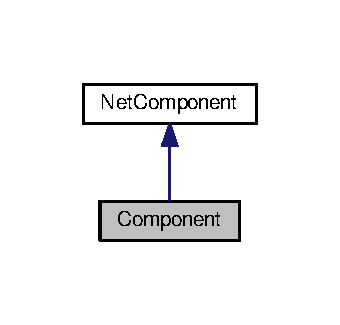
\includegraphics[width=163pt]{class_component__inherit__graph}
\end{center}
\end{figure}


Collaboration diagram for Component\+:\nopagebreak
\begin{figure}[H]
\begin{center}
\leavevmode
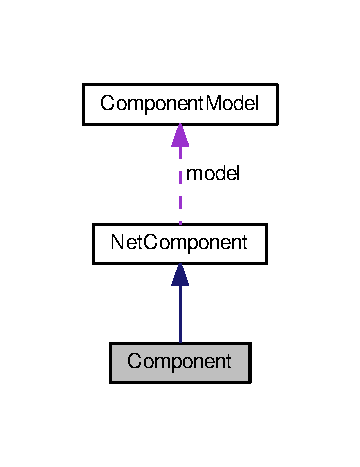
\includegraphics[width=173pt]{class_component__coll__graph}
\end{center}
\end{figure}
\subsection*{Public Member Functions}
\begin{DoxyCompactItemize}
\item 
\hyperlink{class_component_a8775db6d1a2c1afc2e77cd3c8f39da6f}{Component} ()\hypertarget{class_component_a8775db6d1a2c1afc2e77cd3c8f39da6f}{}\label{class_component_a8775db6d1a2c1afc2e77cd3c8f39da6f}

\begin{DoxyCompactList}\small\item\em \hyperlink{class_component}{Component} default constructor. \end{DoxyCompactList}\item 
\hyperlink{class_component_a5c645611542c6f3af559645f699b2806}{Component} (std\+::string str)
\begin{DoxyCompactList}\small\item\em \hyperlink{class_component}{Component} constructor with id. \end{DoxyCompactList}\item 
astl\+::\+D\+F\+A\+\_\+map$<$ \hyperlink{class_sys_transition}{Sys\+Transition}, \hyperlink{class_state_data__str}{State\+Data\+\_\+str} $>$ $\ast$ \hyperlink{class_component_a05d5dfb1fb2fd6f434e58fa286d4b993}{get\+\_\+automaton} () const 
\begin{DoxyCompactList}\small\item\em get\+\_\+automaton \end{DoxyCompactList}\item 
vector$<$ \hyperlink{class_terminal}{Terminal} $\ast$ $>$ \hyperlink{class_component_a812ded651f64b6cbc476ac28cae2fab2}{get\+\_\+input\+\_\+terminals} () const 
\begin{DoxyCompactList}\small\item\em get\+\_\+input\+\_\+terminals \end{DoxyCompactList}\item 
vector$<$ \hyperlink{class_terminal}{Terminal} $\ast$ $>$ \hyperlink{class_component_ae1e4892775ca02ee2a4b727d56edf3a4}{get\+\_\+output\+\_\+terminals} () const 
\begin{DoxyCompactList}\small\item\em get\+\_\+output\+\_\+terminals \end{DoxyCompactList}\item 
void \hyperlink{class_component_a97c16a49225019a6a2b082c006822f8e}{set\+\_\+automaton} (astl\+::\+D\+F\+A\+\_\+map$<$ \hyperlink{class_sys_transition}{Sys\+Transition}, \hyperlink{class_state_data__str}{State\+Data\+\_\+str} $>$ $\ast$autom)
\begin{DoxyCompactList}\small\item\em set\+\_\+automaton \end{DoxyCompactList}\item 
void \hyperlink{class_component_ae16ece39192fc71a468e74b7ee3c340b}{add\+\_\+input\+\_\+term} (\hyperlink{class_terminal}{Terminal} $\ast$t)
\begin{DoxyCompactList}\small\item\em add\+\_\+input\+\_\+term \end{DoxyCompactList}\item 
void \hyperlink{class_component_ad3d6d9f87552e06409bb759b26743a9d}{add\+\_\+output\+\_\+term} (\hyperlink{class_terminal}{Terminal} $\ast$t)
\begin{DoxyCompactList}\small\item\em add\+\_\+output\+\_\+term \end{DoxyCompactList}\item 
\hyperlink{class_terminal}{Terminal} $\ast$ \hyperlink{class_component_ab62c61e09476eea98a5ffd48acdbd11a}{find\+\_\+input\+\_\+terminal} (std\+::string id)
\begin{DoxyCompactList}\small\item\em find\+\_\+input\+\_\+terminal find input terminal from id \end{DoxyCompactList}\item 
\hyperlink{class_terminal}{Terminal} $\ast$ \hyperlink{class_component_ac4e822092e193ccf5c2416dcaf2a4982}{find\+\_\+output\+\_\+terminal} (std\+::string id)
\begin{DoxyCompactList}\small\item\em find\+\_\+output\+\_\+terminal find output terminal from id \end{DoxyCompactList}\item 
bool \hyperlink{class_component_a4ad3ccb5711e8d27c3488b6d353e6426}{operator==} (const \hyperlink{class_component}{Component} c) const 
\begin{DoxyCompactList}\small\item\em operator == overload of equality operator \end{DoxyCompactList}\end{DoxyCompactItemize}
\subsection*{Friends}
\begin{DoxyCompactItemize}
\item 
class {\bfseries boost\+::serialization\+::access}\hypertarget{class_component_ac98d07dd8f7b70e16ccb9a01abf56b9c}{}\label{class_component_ac98d07dd8f7b70e16ccb9a01abf56b9c}

\end{DoxyCompactItemize}
\subsection*{Additional Inherited Members}


\subsection{Detailed Description}
The \hyperlink{class_component}{Component} class represents a concrete component in a problem node. 

\begin{DoxyDate}{Date}
Febbraio 2016 
\end{DoxyDate}
\begin{DoxyAuthor}{Author}
Giulio Quarenghi 
\end{DoxyAuthor}


\subsection{Constructor \& Destructor Documentation}
\index{Component@{Component}!Component@{Component}}
\index{Component@{Component}!Component@{Component}}
\subsubsection[{\texorpdfstring{Component(std\+::string str)}{Component(std::string str)}}]{\setlength{\rightskip}{0pt plus 5cm}Component\+::\+Component (
\begin{DoxyParamCaption}
\item[{std\+::string}]{str}
\end{DoxyParamCaption}
)\hspace{0.3cm}{\ttfamily [inline]}}\hypertarget{class_component_a5c645611542c6f3af559645f699b2806}{}\label{class_component_a5c645611542c6f3af559645f699b2806}


\hyperlink{class_component}{Component} constructor with id. 


\begin{DoxyParams}{Parameters}
{\em str} & name \\
\hline
\end{DoxyParams}


\subsection{Member Function Documentation}
\index{Component@{Component}!add\+\_\+input\+\_\+term@{add\+\_\+input\+\_\+term}}
\index{add\+\_\+input\+\_\+term@{add\+\_\+input\+\_\+term}!Component@{Component}}
\subsubsection[{\texorpdfstring{add\+\_\+input\+\_\+term(\+Terminal $\ast$t)}{add_input_term(Terminal *t)}}]{\setlength{\rightskip}{0pt plus 5cm}void Component\+::add\+\_\+input\+\_\+term (
\begin{DoxyParamCaption}
\item[{{\bf Terminal} $\ast$}]{t}
\end{DoxyParamCaption}
)}\hypertarget{class_component_ae16ece39192fc71a468e74b7ee3c340b}{}\label{class_component_ae16ece39192fc71a468e74b7ee3c340b}


add\+\_\+input\+\_\+term 


\begin{DoxyParams}{Parameters}
{\em t} & \\
\hline
\end{DoxyParams}
\index{Component@{Component}!add\+\_\+output\+\_\+term@{add\+\_\+output\+\_\+term}}
\index{add\+\_\+output\+\_\+term@{add\+\_\+output\+\_\+term}!Component@{Component}}
\subsubsection[{\texorpdfstring{add\+\_\+output\+\_\+term(\+Terminal $\ast$t)}{add_output_term(Terminal *t)}}]{\setlength{\rightskip}{0pt plus 5cm}void Component\+::add\+\_\+output\+\_\+term (
\begin{DoxyParamCaption}
\item[{{\bf Terminal} $\ast$}]{t}
\end{DoxyParamCaption}
)}\hypertarget{class_component_ad3d6d9f87552e06409bb759b26743a9d}{}\label{class_component_ad3d6d9f87552e06409bb759b26743a9d}


add\+\_\+output\+\_\+term 


\begin{DoxyParams}{Parameters}
{\em t} & \\
\hline
\end{DoxyParams}
\index{Component@{Component}!find\+\_\+input\+\_\+terminal@{find\+\_\+input\+\_\+terminal}}
\index{find\+\_\+input\+\_\+terminal@{find\+\_\+input\+\_\+terminal}!Component@{Component}}
\subsubsection[{\texorpdfstring{find\+\_\+input\+\_\+terminal(std\+::string id)}{find_input_terminal(std::string id)}}]{\setlength{\rightskip}{0pt plus 5cm}{\bf Terminal} $\ast$ Component\+::find\+\_\+input\+\_\+terminal (
\begin{DoxyParamCaption}
\item[{std\+::string}]{id}
\end{DoxyParamCaption}
)}\hypertarget{class_component_ab62c61e09476eea98a5ffd48acdbd11a}{}\label{class_component_ab62c61e09476eea98a5ffd48acdbd11a}


find\+\_\+input\+\_\+terminal find input terminal from id 


\begin{DoxyParams}{Parameters}
{\em id} & name of terminal \\
\hline
\end{DoxyParams}
\begin{DoxyReturn}{Returns}
pointer to \hyperlink{class_terminal}{Terminal} 
\end{DoxyReturn}
\index{Component@{Component}!find\+\_\+output\+\_\+terminal@{find\+\_\+output\+\_\+terminal}}
\index{find\+\_\+output\+\_\+terminal@{find\+\_\+output\+\_\+terminal}!Component@{Component}}
\subsubsection[{\texorpdfstring{find\+\_\+output\+\_\+terminal(std\+::string id)}{find_output_terminal(std::string id)}}]{\setlength{\rightskip}{0pt plus 5cm}{\bf Terminal} $\ast$ Component\+::find\+\_\+output\+\_\+terminal (
\begin{DoxyParamCaption}
\item[{std\+::string}]{id}
\end{DoxyParamCaption}
)}\hypertarget{class_component_ac4e822092e193ccf5c2416dcaf2a4982}{}\label{class_component_ac4e822092e193ccf5c2416dcaf2a4982}


find\+\_\+output\+\_\+terminal find output terminal from id 


\begin{DoxyParams}{Parameters}
{\em id} & name \\
\hline
\end{DoxyParams}
\begin{DoxyReturn}{Returns}
pointer to \hyperlink{class_terminal}{Terminal} 
\end{DoxyReturn}
\index{Component@{Component}!get\+\_\+automaton@{get\+\_\+automaton}}
\index{get\+\_\+automaton@{get\+\_\+automaton}!Component@{Component}}
\subsubsection[{\texorpdfstring{get\+\_\+automaton() const }{get_automaton() const }}]{\setlength{\rightskip}{0pt plus 5cm}astl\+::\+D\+F\+A\+\_\+map$<$ {\bf Sys\+Transition}, {\bf State\+Data\+\_\+str} $>$ $\ast$ Component\+::get\+\_\+automaton (
\begin{DoxyParamCaption}
{}
\end{DoxyParamCaption}
) const}\hypertarget{class_component_a05d5dfb1fb2fd6f434e58fa286d4b993}{}\label{class_component_a05d5dfb1fb2fd6f434e58fa286d4b993}


get\+\_\+automaton 

\begin{DoxyReturn}{Returns}

\end{DoxyReturn}
\index{Component@{Component}!get\+\_\+input\+\_\+terminals@{get\+\_\+input\+\_\+terminals}}
\index{get\+\_\+input\+\_\+terminals@{get\+\_\+input\+\_\+terminals}!Component@{Component}}
\subsubsection[{\texorpdfstring{get\+\_\+input\+\_\+terminals() const }{get_input_terminals() const }}]{\setlength{\rightskip}{0pt plus 5cm}vector$<$ {\bf Terminal} $\ast$ $>$ Component\+::get\+\_\+input\+\_\+terminals (
\begin{DoxyParamCaption}
{}
\end{DoxyParamCaption}
) const}\hypertarget{class_component_a812ded651f64b6cbc476ac28cae2fab2}{}\label{class_component_a812ded651f64b6cbc476ac28cae2fab2}


get\+\_\+input\+\_\+terminals 

\begin{DoxyReturn}{Returns}

\end{DoxyReturn}
\index{Component@{Component}!get\+\_\+output\+\_\+terminals@{get\+\_\+output\+\_\+terminals}}
\index{get\+\_\+output\+\_\+terminals@{get\+\_\+output\+\_\+terminals}!Component@{Component}}
\subsubsection[{\texorpdfstring{get\+\_\+output\+\_\+terminals() const }{get_output_terminals() const }}]{\setlength{\rightskip}{0pt plus 5cm}vector$<$ {\bf Terminal} $\ast$ $>$ Component\+::get\+\_\+output\+\_\+terminals (
\begin{DoxyParamCaption}
{}
\end{DoxyParamCaption}
) const}\hypertarget{class_component_ae1e4892775ca02ee2a4b727d56edf3a4}{}\label{class_component_ae1e4892775ca02ee2a4b727d56edf3a4}


get\+\_\+output\+\_\+terminals 

\begin{DoxyReturn}{Returns}

\end{DoxyReturn}
\index{Component@{Component}!operator==@{operator==}}
\index{operator==@{operator==}!Component@{Component}}
\subsubsection[{\texorpdfstring{operator==(const Component c) const }{operator==(const Component c) const }}]{\setlength{\rightskip}{0pt plus 5cm}bool Component\+::operator== (
\begin{DoxyParamCaption}
\item[{const {\bf Component}}]{c}
\end{DoxyParamCaption}
) const\hspace{0.3cm}{\ttfamily [inline]}}\hypertarget{class_component_a4ad3ccb5711e8d27c3488b6d353e6426}{}\label{class_component_a4ad3ccb5711e8d27c3488b6d353e6426}


operator == overload of equality operator 


\begin{DoxyParams}{Parameters}
{\em c} & \\
\hline
\end{DoxyParams}
\begin{DoxyReturn}{Returns}

\end{DoxyReturn}
\index{Component@{Component}!set\+\_\+automaton@{set\+\_\+automaton}}
\index{set\+\_\+automaton@{set\+\_\+automaton}!Component@{Component}}
\subsubsection[{\texorpdfstring{set\+\_\+automaton(astl\+::\+D\+F\+A\+\_\+map$<$ Sys\+Transition, State\+Data\+\_\+str $>$ $\ast$autom)}{set_automaton(astl::DFA_map< SysTransition, StateData_str > *autom)}}]{\setlength{\rightskip}{0pt plus 5cm}void Component\+::set\+\_\+automaton (
\begin{DoxyParamCaption}
\item[{astl\+::\+D\+F\+A\+\_\+map$<$ {\bf Sys\+Transition}, {\bf State\+Data\+\_\+str} $>$ $\ast$}]{autom}
\end{DoxyParamCaption}
)}\hypertarget{class_component_a97c16a49225019a6a2b082c006822f8e}{}\label{class_component_a97c16a49225019a6a2b082c006822f8e}


set\+\_\+automaton 


\begin{DoxyParams}{Parameters}
{\em autom} & \\
\hline
\end{DoxyParams}


The documentation for this class was generated from the following files\+:\begin{DoxyCompactItemize}
\item 
component.\+h\item 
component.\+cpp\end{DoxyCompactItemize}

\hypertarget{class_component_model}{}\section{Component\+Model Class Reference}
\label{class_component_model}\index{Component\+Model@{Component\+Model}}


The \hyperlink{class_component_model}{Component\+Model} class.  




{\ttfamily \#include $<$componentmodel.\+h$>$}

\subsection*{Public Member Functions}
\begin{DoxyCompactItemize}
\item 
\hyperlink{class_component_model_a8df1c9db45b776c8447300b6ff1845ac}{Component\+Model} ()\hypertarget{class_component_model_a8df1c9db45b776c8447300b6ff1845ac}{}\label{class_component_model_a8df1c9db45b776c8447300b6ff1845ac}

\begin{DoxyCompactList}\small\item\em \hyperlink{class_component_model}{Component\+Model} default constructor. \end{DoxyCompactList}\item 
\hyperlink{class_component_model_a4a2b81f18a4109a2510da0441bd6dd92}{Component\+Model} (std\+::string str)
\begin{DoxyCompactList}\small\item\em \hyperlink{class_component_model}{Component\+Model} constructor from id. \end{DoxyCompactList}\item 
std\+::string \hyperlink{class_component_model_a8827d16c2751dc3ec2e876bd219c81f4}{get\+\_\+name} () const 
\begin{DoxyCompactList}\small\item\em get\+\_\+name \end{DoxyCompactList}\item 
vector$<$ std\+::string $>$ \hyperlink{class_component_model_a0e405f2d7095cb12c48994a7028e5a49}{get\+\_\+events} () const 
\begin{DoxyCompactList}\small\item\em get\+\_\+events \end{DoxyCompactList}\item 
vector$<$ std\+::string $>$ \hyperlink{class_component_model_a59727fd988b5adddd5e769500720c99a}{get\+\_\+inputs} () const 
\begin{DoxyCompactList}\small\item\em get\+\_\+inputs \end{DoxyCompactList}\item 
vector$<$ std\+::string $>$ \hyperlink{class_component_model_afbdb01b399354b308d61ae1393cbec63}{get\+\_\+outputs} () const 
\begin{DoxyCompactList}\small\item\em get\+\_\+outputs \end{DoxyCompactList}\item 
vector$<$ std\+::string $>$ \hyperlink{class_component_model_a7960473e775b4dbbc0ddcc0c89bc2d20}{get\+\_\+states} () const 
\begin{DoxyCompactList}\small\item\em get\+\_\+states \end{DoxyCompactList}\item 
vector$<$ \hyperlink{class_transition}{Transition} $>$ \hyperlink{class_component_model_ad35b6b75698b8eeeee0e59b994e6292a}{get\+\_\+trans} () const 
\begin{DoxyCompactList}\small\item\em get\+\_\+trans \end{DoxyCompactList}\item 
astl\+::\+D\+F\+A\+\_\+map$<$ \hyperlink{class_transition}{Transition}, \hyperlink{class_state_data__str}{State\+Data\+\_\+str} $>$ $\ast$ \hyperlink{class_component_model_a6ebfb1ee56c82313e9305462e29d0fc1}{get\+\_\+automaton} () const 
\begin{DoxyCompactList}\small\item\em get\+\_\+automaton \end{DoxyCompactList}\item 
void \hyperlink{class_component_model_a62c871017dcb565d2ffea30f2bf64eab}{set\+\_\+events} (vector$<$ std\+::string $>$ v)
\begin{DoxyCompactList}\small\item\em set\+\_\+events \end{DoxyCompactList}\item 
void \hyperlink{class_component_model_a6066f9a643b19ce2a3a8922c957db8d1}{set\+\_\+inputs} (vector$<$ std\+::string $>$ v)
\begin{DoxyCompactList}\small\item\em set\+\_\+inputs \end{DoxyCompactList}\item 
void \hyperlink{class_component_model_ae87ec7dc958cfc89815472970d90fdc6}{set\+\_\+outputs} (vector$<$ std\+::string $>$ v)
\begin{DoxyCompactList}\small\item\em set\+\_\+outputs \end{DoxyCompactList}\item 
void \hyperlink{class_component_model_ac5510406a3ebbc0aec567973d9f02d44}{set\+\_\+states} (vector$<$ std\+::string $>$ v)
\begin{DoxyCompactList}\small\item\em set\+\_\+states \end{DoxyCompactList}\item 
void \hyperlink{class_component_model_a7ccd13a1905914b08d079ac3e89d7ef9}{set\+\_\+trans} (vector$<$ \hyperlink{class_transition}{Transition} $>$ v)
\begin{DoxyCompactList}\small\item\em set\+\_\+trans \end{DoxyCompactList}\item 
void \hyperlink{class_component_model_a0c56c8a83e2af3bf68bc5bd820607ed5}{add\+\_\+event} (std\+::string ev)
\begin{DoxyCompactList}\small\item\em add\+\_\+event \end{DoxyCompactList}\item 
void \hyperlink{class_component_model_a4f7421bbe94259bc579d05b197a4885d}{add\+\_\+input} (std\+::string in)
\begin{DoxyCompactList}\small\item\em add\+\_\+input \end{DoxyCompactList}\item 
void \hyperlink{class_component_model_a759f3d8b44dc9d50242dc2914f8d2302}{add\+\_\+output} (std\+::string out)
\begin{DoxyCompactList}\small\item\em add\+\_\+output \end{DoxyCompactList}\item 
void \hyperlink{class_component_model_a018585d39632c1137fccdd5a636fc429}{add\+\_\+state} (std\+::string st)
\begin{DoxyCompactList}\small\item\em add\+\_\+state \end{DoxyCompactList}\item 
void \hyperlink{class_component_model_a60a971d9497c283d1b53b19955197d2e}{build\+\_\+automaton} ()\hypertarget{class_component_model_a60a971d9497c283d1b53b19955197d2e}{}\label{class_component_model_a60a971d9497c283d1b53b19955197d2e}

\begin{DoxyCompactList}\small\item\em build\+\_\+automaton \end{DoxyCompactList}\item 
astl\+::\+D\+F\+A\+\_\+map$<$ \hyperlink{class_transition}{Transition}, \hyperlink{class_state_data__str}{State\+Data\+\_\+str} $>$\+::state\+\_\+type \hyperlink{class_component_model_a1dce877ed60027f1346b521d848d0889}{find\+\_\+state} (std\+::string name)
\begin{DoxyCompactList}\small\item\em find\+\_\+state from name \end{DoxyCompactList}\item 
\hyperlink{class_transition}{Transition} $\ast$ \hyperlink{class_component_model_a3788c218834cffc04c0cd4239364c7df}{find\+\_\+trans} (std\+::string name\+\_\+tr)
\begin{DoxyCompactList}\small\item\em find\+\_\+trans finds transition from id \end{DoxyCompactList}\end{DoxyCompactItemize}
\subsection*{Friends}
\begin{DoxyCompactItemize}
\item 
class {\bfseries boost\+::serialization\+::access}\hypertarget{class_component_model_ac98d07dd8f7b70e16ccb9a01abf56b9c}{}\label{class_component_model_ac98d07dd8f7b70e16ccb9a01abf56b9c}

\end{DoxyCompactItemize}


\subsection{Detailed Description}
The \hyperlink{class_component_model}{Component\+Model} class. 

\begin{DoxyDate}{Date}
Febbraio 2016 
\end{DoxyDate}
\begin{DoxyAuthor}{Author}
Giulio Quarenghi 
\end{DoxyAuthor}


\subsection{Constructor \& Destructor Documentation}
\index{Component\+Model@{Component\+Model}!Component\+Model@{Component\+Model}}
\index{Component\+Model@{Component\+Model}!Component\+Model@{Component\+Model}}
\subsubsection[{\texorpdfstring{Component\+Model(std\+::string str)}{ComponentModel(std::string str)}}]{\setlength{\rightskip}{0pt plus 5cm}Component\+Model\+::\+Component\+Model (
\begin{DoxyParamCaption}
\item[{std\+::string}]{str}
\end{DoxyParamCaption}
)\hspace{0.3cm}{\ttfamily [inline]}}\hypertarget{class_component_model_a4a2b81f18a4109a2510da0441bd6dd92}{}\label{class_component_model_a4a2b81f18a4109a2510da0441bd6dd92}


\hyperlink{class_component_model}{Component\+Model} constructor from id. 


\begin{DoxyParams}{Parameters}
{\em str} & \\
\hline
\end{DoxyParams}


\subsection{Member Function Documentation}
\index{Component\+Model@{Component\+Model}!add\+\_\+event@{add\+\_\+event}}
\index{add\+\_\+event@{add\+\_\+event}!Component\+Model@{Component\+Model}}
\subsubsection[{\texorpdfstring{add\+\_\+event(std\+::string ev)}{add_event(std::string ev)}}]{\setlength{\rightskip}{0pt plus 5cm}void Component\+Model\+::add\+\_\+event (
\begin{DoxyParamCaption}
\item[{std\+::string}]{ev}
\end{DoxyParamCaption}
)}\hypertarget{class_component_model_a0c56c8a83e2af3bf68bc5bd820607ed5}{}\label{class_component_model_a0c56c8a83e2af3bf68bc5bd820607ed5}


add\+\_\+event 


\begin{DoxyParams}{Parameters}
{\em ev} & \\
\hline
\end{DoxyParams}
\index{Component\+Model@{Component\+Model}!add\+\_\+input@{add\+\_\+input}}
\index{add\+\_\+input@{add\+\_\+input}!Component\+Model@{Component\+Model}}
\subsubsection[{\texorpdfstring{add\+\_\+input(std\+::string in)}{add_input(std::string in)}}]{\setlength{\rightskip}{0pt plus 5cm}void Component\+Model\+::add\+\_\+input (
\begin{DoxyParamCaption}
\item[{std\+::string}]{in}
\end{DoxyParamCaption}
)}\hypertarget{class_component_model_a4f7421bbe94259bc579d05b197a4885d}{}\label{class_component_model_a4f7421bbe94259bc579d05b197a4885d}


add\+\_\+input 


\begin{DoxyParams}{Parameters}
{\em in} & \\
\hline
\end{DoxyParams}
\index{Component\+Model@{Component\+Model}!add\+\_\+output@{add\+\_\+output}}
\index{add\+\_\+output@{add\+\_\+output}!Component\+Model@{Component\+Model}}
\subsubsection[{\texorpdfstring{add\+\_\+output(std\+::string out)}{add_output(std::string out)}}]{\setlength{\rightskip}{0pt plus 5cm}void Component\+Model\+::add\+\_\+output (
\begin{DoxyParamCaption}
\item[{std\+::string}]{out}
\end{DoxyParamCaption}
)}\hypertarget{class_component_model_a759f3d8b44dc9d50242dc2914f8d2302}{}\label{class_component_model_a759f3d8b44dc9d50242dc2914f8d2302}


add\+\_\+output 


\begin{DoxyParams}{Parameters}
{\em out} & \\
\hline
\end{DoxyParams}
\index{Component\+Model@{Component\+Model}!add\+\_\+state@{add\+\_\+state}}
\index{add\+\_\+state@{add\+\_\+state}!Component\+Model@{Component\+Model}}
\subsubsection[{\texorpdfstring{add\+\_\+state(std\+::string st)}{add_state(std::string st)}}]{\setlength{\rightskip}{0pt plus 5cm}void Component\+Model\+::add\+\_\+state (
\begin{DoxyParamCaption}
\item[{std\+::string}]{st}
\end{DoxyParamCaption}
)}\hypertarget{class_component_model_a018585d39632c1137fccdd5a636fc429}{}\label{class_component_model_a018585d39632c1137fccdd5a636fc429}


add\+\_\+state 


\begin{DoxyParams}{Parameters}
{\em st} & \\
\hline
\end{DoxyParams}
\index{Component\+Model@{Component\+Model}!find\+\_\+state@{find\+\_\+state}}
\index{find\+\_\+state@{find\+\_\+state}!Component\+Model@{Component\+Model}}
\subsubsection[{\texorpdfstring{find\+\_\+state(std\+::string name)}{find_state(std::string name)}}]{\setlength{\rightskip}{0pt plus 5cm}D\+F\+A\+\_\+map$<$ {\bf Transition}, {\bf State\+Data\+\_\+str} $>$\+::state\+\_\+type Component\+Model\+::find\+\_\+state (
\begin{DoxyParamCaption}
\item[{std\+::string}]{name}
\end{DoxyParamCaption}
)}\hypertarget{class_component_model_a1dce877ed60027f1346b521d848d0889}{}\label{class_component_model_a1dce877ed60027f1346b521d848d0889}


find\+\_\+state from name 


\begin{DoxyParams}{Parameters}
{\em name} & \\
\hline
\end{DoxyParams}
\begin{DoxyReturn}{Returns}
automaton state 
\end{DoxyReturn}
\index{Component\+Model@{Component\+Model}!find\+\_\+trans@{find\+\_\+trans}}
\index{find\+\_\+trans@{find\+\_\+trans}!Component\+Model@{Component\+Model}}
\subsubsection[{\texorpdfstring{find\+\_\+trans(std\+::string name\+\_\+tr)}{find_trans(std::string name_tr)}}]{\setlength{\rightskip}{0pt plus 5cm}{\bf Transition} $\ast$ Component\+Model\+::find\+\_\+trans (
\begin{DoxyParamCaption}
\item[{std\+::string}]{name\+\_\+tr}
\end{DoxyParamCaption}
)}\hypertarget{class_component_model_a3788c218834cffc04c0cd4239364c7df}{}\label{class_component_model_a3788c218834cffc04c0cd4239364c7df}


find\+\_\+trans finds transition from id 


\begin{DoxyParams}{Parameters}
{\em name\+\_\+tr} & transition name \\
\hline
\end{DoxyParams}
\begin{DoxyReturn}{Returns}
pointer to \hyperlink{class_transition}{Transition} 
\end{DoxyReturn}
\index{Component\+Model@{Component\+Model}!get\+\_\+automaton@{get\+\_\+automaton}}
\index{get\+\_\+automaton@{get\+\_\+automaton}!Component\+Model@{Component\+Model}}
\subsubsection[{\texorpdfstring{get\+\_\+automaton() const }{get_automaton() const }}]{\setlength{\rightskip}{0pt plus 5cm}astl\+::\+D\+F\+A\+\_\+map$<$ {\bf Transition}, {\bf State\+Data\+\_\+str} $>$ $\ast$ Component\+Model\+::get\+\_\+automaton (
\begin{DoxyParamCaption}
{}
\end{DoxyParamCaption}
) const}\hypertarget{class_component_model_a6ebfb1ee56c82313e9305462e29d0fc1}{}\label{class_component_model_a6ebfb1ee56c82313e9305462e29d0fc1}


get\+\_\+automaton 

\begin{DoxyReturn}{Returns}

\end{DoxyReturn}
\index{Component\+Model@{Component\+Model}!get\+\_\+events@{get\+\_\+events}}
\index{get\+\_\+events@{get\+\_\+events}!Component\+Model@{Component\+Model}}
\subsubsection[{\texorpdfstring{get\+\_\+events() const }{get_events() const }}]{\setlength{\rightskip}{0pt plus 5cm}vector$<$ std\+::string $>$ Component\+Model\+::get\+\_\+events (
\begin{DoxyParamCaption}
{}
\end{DoxyParamCaption}
) const}\hypertarget{class_component_model_a0e405f2d7095cb12c48994a7028e5a49}{}\label{class_component_model_a0e405f2d7095cb12c48994a7028e5a49}


get\+\_\+events 

\begin{DoxyReturn}{Returns}

\end{DoxyReturn}
\index{Component\+Model@{Component\+Model}!get\+\_\+inputs@{get\+\_\+inputs}}
\index{get\+\_\+inputs@{get\+\_\+inputs}!Component\+Model@{Component\+Model}}
\subsubsection[{\texorpdfstring{get\+\_\+inputs() const }{get_inputs() const }}]{\setlength{\rightskip}{0pt plus 5cm}vector$<$ std\+::string $>$ Component\+Model\+::get\+\_\+inputs (
\begin{DoxyParamCaption}
{}
\end{DoxyParamCaption}
) const}\hypertarget{class_component_model_a59727fd988b5adddd5e769500720c99a}{}\label{class_component_model_a59727fd988b5adddd5e769500720c99a}


get\+\_\+inputs 

\begin{DoxyReturn}{Returns}

\end{DoxyReturn}
\index{Component\+Model@{Component\+Model}!get\+\_\+name@{get\+\_\+name}}
\index{get\+\_\+name@{get\+\_\+name}!Component\+Model@{Component\+Model}}
\subsubsection[{\texorpdfstring{get\+\_\+name() const }{get_name() const }}]{\setlength{\rightskip}{0pt plus 5cm}std\+::string Component\+Model\+::get\+\_\+name (
\begin{DoxyParamCaption}
{}
\end{DoxyParamCaption}
) const}\hypertarget{class_component_model_a8827d16c2751dc3ec2e876bd219c81f4}{}\label{class_component_model_a8827d16c2751dc3ec2e876bd219c81f4}


get\+\_\+name 

\begin{DoxyReturn}{Returns}

\end{DoxyReturn}
\index{Component\+Model@{Component\+Model}!get\+\_\+outputs@{get\+\_\+outputs}}
\index{get\+\_\+outputs@{get\+\_\+outputs}!Component\+Model@{Component\+Model}}
\subsubsection[{\texorpdfstring{get\+\_\+outputs() const }{get_outputs() const }}]{\setlength{\rightskip}{0pt plus 5cm}vector$<$ std\+::string $>$ Component\+Model\+::get\+\_\+outputs (
\begin{DoxyParamCaption}
{}
\end{DoxyParamCaption}
) const}\hypertarget{class_component_model_afbdb01b399354b308d61ae1393cbec63}{}\label{class_component_model_afbdb01b399354b308d61ae1393cbec63}


get\+\_\+outputs 

\begin{DoxyReturn}{Returns}

\end{DoxyReturn}
\index{Component\+Model@{Component\+Model}!get\+\_\+states@{get\+\_\+states}}
\index{get\+\_\+states@{get\+\_\+states}!Component\+Model@{Component\+Model}}
\subsubsection[{\texorpdfstring{get\+\_\+states() const }{get_states() const }}]{\setlength{\rightskip}{0pt plus 5cm}vector$<$ std\+::string $>$ Component\+Model\+::get\+\_\+states (
\begin{DoxyParamCaption}
{}
\end{DoxyParamCaption}
) const}\hypertarget{class_component_model_a7960473e775b4dbbc0ddcc0c89bc2d20}{}\label{class_component_model_a7960473e775b4dbbc0ddcc0c89bc2d20}


get\+\_\+states 

\begin{DoxyReturn}{Returns}

\end{DoxyReturn}
\index{Component\+Model@{Component\+Model}!get\+\_\+trans@{get\+\_\+trans}}
\index{get\+\_\+trans@{get\+\_\+trans}!Component\+Model@{Component\+Model}}
\subsubsection[{\texorpdfstring{get\+\_\+trans() const }{get_trans() const }}]{\setlength{\rightskip}{0pt plus 5cm}vector$<$ {\bf Transition} $>$ Component\+Model\+::get\+\_\+trans (
\begin{DoxyParamCaption}
{}
\end{DoxyParamCaption}
) const}\hypertarget{class_component_model_ad35b6b75698b8eeeee0e59b994e6292a}{}\label{class_component_model_ad35b6b75698b8eeeee0e59b994e6292a}


get\+\_\+trans 

\begin{DoxyReturn}{Returns}

\end{DoxyReturn}
\index{Component\+Model@{Component\+Model}!set\+\_\+events@{set\+\_\+events}}
\index{set\+\_\+events@{set\+\_\+events}!Component\+Model@{Component\+Model}}
\subsubsection[{\texorpdfstring{set\+\_\+events(vector$<$ std\+::string $>$ v)}{set_events(vector< std::string > v)}}]{\setlength{\rightskip}{0pt plus 5cm}void Component\+Model\+::set\+\_\+events (
\begin{DoxyParamCaption}
\item[{vector$<$ std\+::string $>$}]{v}
\end{DoxyParamCaption}
)}\hypertarget{class_component_model_a62c871017dcb565d2ffea30f2bf64eab}{}\label{class_component_model_a62c871017dcb565d2ffea30f2bf64eab}


set\+\_\+events 


\begin{DoxyParams}{Parameters}
{\em v} & \\
\hline
\end{DoxyParams}
\index{Component\+Model@{Component\+Model}!set\+\_\+inputs@{set\+\_\+inputs}}
\index{set\+\_\+inputs@{set\+\_\+inputs}!Component\+Model@{Component\+Model}}
\subsubsection[{\texorpdfstring{set\+\_\+inputs(vector$<$ std\+::string $>$ v)}{set_inputs(vector< std::string > v)}}]{\setlength{\rightskip}{0pt plus 5cm}void Component\+Model\+::set\+\_\+inputs (
\begin{DoxyParamCaption}
\item[{vector$<$ std\+::string $>$}]{v}
\end{DoxyParamCaption}
)}\hypertarget{class_component_model_a6066f9a643b19ce2a3a8922c957db8d1}{}\label{class_component_model_a6066f9a643b19ce2a3a8922c957db8d1}


set\+\_\+inputs 


\begin{DoxyParams}{Parameters}
{\em v} & \\
\hline
\end{DoxyParams}
\index{Component\+Model@{Component\+Model}!set\+\_\+outputs@{set\+\_\+outputs}}
\index{set\+\_\+outputs@{set\+\_\+outputs}!Component\+Model@{Component\+Model}}
\subsubsection[{\texorpdfstring{set\+\_\+outputs(vector$<$ std\+::string $>$ v)}{set_outputs(vector< std::string > v)}}]{\setlength{\rightskip}{0pt plus 5cm}void Component\+Model\+::set\+\_\+outputs (
\begin{DoxyParamCaption}
\item[{vector$<$ std\+::string $>$}]{v}
\end{DoxyParamCaption}
)}\hypertarget{class_component_model_ae87ec7dc958cfc89815472970d90fdc6}{}\label{class_component_model_ae87ec7dc958cfc89815472970d90fdc6}


set\+\_\+outputs 


\begin{DoxyParams}{Parameters}
{\em v} & \\
\hline
\end{DoxyParams}
\index{Component\+Model@{Component\+Model}!set\+\_\+states@{set\+\_\+states}}
\index{set\+\_\+states@{set\+\_\+states}!Component\+Model@{Component\+Model}}
\subsubsection[{\texorpdfstring{set\+\_\+states(vector$<$ std\+::string $>$ v)}{set_states(vector< std::string > v)}}]{\setlength{\rightskip}{0pt plus 5cm}void Component\+Model\+::set\+\_\+states (
\begin{DoxyParamCaption}
\item[{vector$<$ std\+::string $>$}]{v}
\end{DoxyParamCaption}
)}\hypertarget{class_component_model_ac5510406a3ebbc0aec567973d9f02d44}{}\label{class_component_model_ac5510406a3ebbc0aec567973d9f02d44}


set\+\_\+states 


\begin{DoxyParams}{Parameters}
{\em v} & \\
\hline
\end{DoxyParams}
\index{Component\+Model@{Component\+Model}!set\+\_\+trans@{set\+\_\+trans}}
\index{set\+\_\+trans@{set\+\_\+trans}!Component\+Model@{Component\+Model}}
\subsubsection[{\texorpdfstring{set\+\_\+trans(vector$<$ Transition $>$ v)}{set_trans(vector< Transition > v)}}]{\setlength{\rightskip}{0pt plus 5cm}void Component\+Model\+::set\+\_\+trans (
\begin{DoxyParamCaption}
\item[{vector$<$ {\bf Transition} $>$}]{v}
\end{DoxyParamCaption}
)}\hypertarget{class_component_model_a7ccd13a1905914b08d079ac3e89d7ef9}{}\label{class_component_model_a7ccd13a1905914b08d079ac3e89d7ef9}


set\+\_\+trans 


\begin{DoxyParams}{Parameters}
{\em v} & \\
\hline
\end{DoxyParams}


The documentation for this class was generated from the following files\+:\begin{DoxyCompactItemize}
\item 
componentmodel.\+h\item 
componentmodel.\+cpp\end{DoxyCompactItemize}

\hypertarget{class_net_component}{}\section{Net\+Component Class Reference}
\label{class_net_component}\index{Net\+Component@{Net\+Component}}


The \hyperlink{class_net_component}{Net\+Component} class represents a component in a network model.  




{\ttfamily \#include $<$netcomponent.\+h$>$}



Inheritance diagram for Net\+Component\+:\nopagebreak
\begin{figure}[H]
\begin{center}
\leavevmode
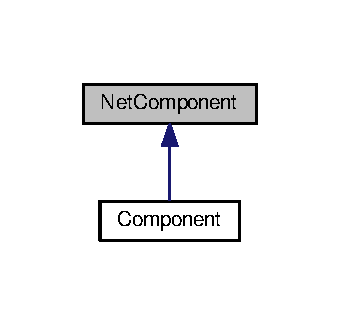
\includegraphics[width=163pt]{class_net_component__inherit__graph}
\end{center}
\end{figure}


Collaboration diagram for Net\+Component\+:\nopagebreak
\begin{figure}[H]
\begin{center}
\leavevmode
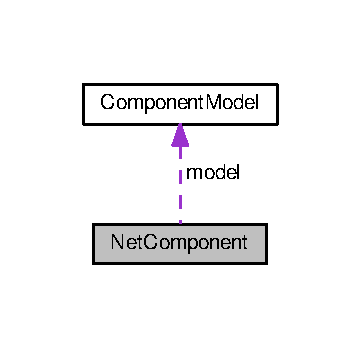
\includegraphics[width=173pt]{class_net_component__coll__graph}
\end{center}
\end{figure}
\subsection*{Public Member Functions}
\begin{DoxyCompactItemize}
\item 
\hyperlink{class_net_component_a77dc2a06629c0cbbe1b2ce1c33ae34f7}{Net\+Component} ()\hypertarget{class_net_component_a77dc2a06629c0cbbe1b2ce1c33ae34f7}{}\label{class_net_component_a77dc2a06629c0cbbe1b2ce1c33ae34f7}

\begin{DoxyCompactList}\small\item\em \hyperlink{class_net_component}{Net\+Component} default constructor. \end{DoxyCompactList}\item 
\hyperlink{class_net_component_aa1b768bd499286c1ee62202d5fe36e7c}{Net\+Component} (std\+::string str)
\begin{DoxyCompactList}\small\item\em \hyperlink{class_net_component}{Net\+Component} constructor from id. \end{DoxyCompactList}\item 
std\+::string \hyperlink{class_net_component_a04ae33a17be08247e96bee14775d31e6}{get\+\_\+name} () const 
\begin{DoxyCompactList}\small\item\em get\+\_\+name \end{DoxyCompactList}\item 
\hyperlink{class_component_model}{Component\+Model} $\ast$ \hyperlink{class_net_component_a94adff8ef99b5283f7768f13e54c538a}{get\+\_\+model} () const 
\begin{DoxyCompactList}\small\item\em get\+\_\+model \end{DoxyCompactList}\item 
void \hyperlink{class_net_component_a82a52610414f1913eb4711d5ad63f66c}{set\+\_\+model} (\hyperlink{class_component_model}{Component\+Model} $\ast$cm)
\begin{DoxyCompactList}\small\item\em set\+\_\+model assigns model \end{DoxyCompactList}\item 
bool \hyperlink{class_net_component_ad810dbc0fc141639e872ca7526d29b0e}{operator==} (const \hyperlink{class_net_component}{Net\+Component} c) const 
\begin{DoxyCompactList}\small\item\em operator == overload of equality operator \end{DoxyCompactList}\end{DoxyCompactItemize}
\subsection*{Protected Member Functions}
\begin{DoxyCompactItemize}
\item 
{\footnotesize template$<$class Archive $>$ }\\void {\bfseries serialize} (Archive \&ar, const unsigned int version)\hypertarget{class_net_component_af55f6a28639ad956b41a21e73e16f445}{}\label{class_net_component_af55f6a28639ad956b41a21e73e16f445}

\end{DoxyCompactItemize}
\subsection*{Protected Attributes}
\begin{DoxyCompactItemize}
\item 
std\+::string \hyperlink{class_net_component_aa1fd04ed705210806544993b51fffb0f}{name}\hypertarget{class_net_component_aa1fd04ed705210806544993b51fffb0f}{}\label{class_net_component_aa1fd04ed705210806544993b51fffb0f}

\begin{DoxyCompactList}\small\item\em name \end{DoxyCompactList}\item 
\hyperlink{class_component_model}{Component\+Model} $\ast$ \hyperlink{class_net_component_a7fec3d6449003b423d617529e337a7f5}{model}\hypertarget{class_net_component_a7fec3d6449003b423d617529e337a7f5}{}\label{class_net_component_a7fec3d6449003b423d617529e337a7f5}

\begin{DoxyCompactList}\small\item\em model component model \end{DoxyCompactList}\end{DoxyCompactItemize}
\subsection*{Friends}
\begin{DoxyCompactItemize}
\item 
class {\bfseries boost\+::serialization\+::access}\hypertarget{class_net_component_ac98d07dd8f7b70e16ccb9a01abf56b9c}{}\label{class_net_component_ac98d07dd8f7b70e16ccb9a01abf56b9c}

\end{DoxyCompactItemize}


\subsection{Detailed Description}
The \hyperlink{class_net_component}{Net\+Component} class represents a component in a network model. 

\begin{DoxyDate}{Date}
Febbraio 2016 
\end{DoxyDate}
\begin{DoxyAuthor}{Author}
Giulio Quarenghi 
\end{DoxyAuthor}


\subsection{Constructor \& Destructor Documentation}
\index{Net\+Component@{Net\+Component}!Net\+Component@{Net\+Component}}
\index{Net\+Component@{Net\+Component}!Net\+Component@{Net\+Component}}
\subsubsection[{\texorpdfstring{Net\+Component(std\+::string str)}{NetComponent(std::string str)}}]{\setlength{\rightskip}{0pt plus 5cm}Net\+Component\+::\+Net\+Component (
\begin{DoxyParamCaption}
\item[{std\+::string}]{str}
\end{DoxyParamCaption}
)}\hypertarget{class_net_component_aa1b768bd499286c1ee62202d5fe36e7c}{}\label{class_net_component_aa1b768bd499286c1ee62202d5fe36e7c}


\hyperlink{class_net_component}{Net\+Component} constructor from id. 


\begin{DoxyParams}{Parameters}
{\em str} & name \\
\hline
\end{DoxyParams}


\subsection{Member Function Documentation}
\index{Net\+Component@{Net\+Component}!get\+\_\+model@{get\+\_\+model}}
\index{get\+\_\+model@{get\+\_\+model}!Net\+Component@{Net\+Component}}
\subsubsection[{\texorpdfstring{get\+\_\+model() const }{get_model() const }}]{\setlength{\rightskip}{0pt plus 5cm}{\bf Component\+Model} $\ast$ Net\+Component\+::get\+\_\+model (
\begin{DoxyParamCaption}
{}
\end{DoxyParamCaption}
) const}\hypertarget{class_net_component_a94adff8ef99b5283f7768f13e54c538a}{}\label{class_net_component_a94adff8ef99b5283f7768f13e54c538a}


get\+\_\+model 

\begin{DoxyReturn}{Returns}
pointer to \hyperlink{class_component_model}{Component\+Model} 
\end{DoxyReturn}
\index{Net\+Component@{Net\+Component}!get\+\_\+name@{get\+\_\+name}}
\index{get\+\_\+name@{get\+\_\+name}!Net\+Component@{Net\+Component}}
\subsubsection[{\texorpdfstring{get\+\_\+name() const }{get_name() const }}]{\setlength{\rightskip}{0pt plus 5cm}std\+::string Net\+Component\+::get\+\_\+name (
\begin{DoxyParamCaption}
{}
\end{DoxyParamCaption}
) const}\hypertarget{class_net_component_a04ae33a17be08247e96bee14775d31e6}{}\label{class_net_component_a04ae33a17be08247e96bee14775d31e6}


get\+\_\+name 

\begin{DoxyReturn}{Returns}

\end{DoxyReturn}
\index{Net\+Component@{Net\+Component}!operator==@{operator==}}
\index{operator==@{operator==}!Net\+Component@{Net\+Component}}
\subsubsection[{\texorpdfstring{operator==(const Net\+Component c) const }{operator==(const NetComponent c) const }}]{\setlength{\rightskip}{0pt plus 5cm}bool Net\+Component\+::operator== (
\begin{DoxyParamCaption}
\item[{const {\bf Net\+Component}}]{c}
\end{DoxyParamCaption}
) const\hspace{0.3cm}{\ttfamily [inline]}}\hypertarget{class_net_component_ad810dbc0fc141639e872ca7526d29b0e}{}\label{class_net_component_ad810dbc0fc141639e872ca7526d29b0e}


operator == overload of equality operator 


\begin{DoxyParams}{Parameters}
{\em c} & \\
\hline
\end{DoxyParams}
\begin{DoxyReturn}{Returns}

\end{DoxyReturn}
\index{Net\+Component@{Net\+Component}!set\+\_\+model@{set\+\_\+model}}
\index{set\+\_\+model@{set\+\_\+model}!Net\+Component@{Net\+Component}}
\subsubsection[{\texorpdfstring{set\+\_\+model(\+Component\+Model $\ast$cm)}{set_model(ComponentModel *cm)}}]{\setlength{\rightskip}{0pt plus 5cm}void Net\+Component\+::set\+\_\+model (
\begin{DoxyParamCaption}
\item[{{\bf Component\+Model} $\ast$}]{cm}
\end{DoxyParamCaption}
)}\hypertarget{class_net_component_a82a52610414f1913eb4711d5ad63f66c}{}\label{class_net_component_a82a52610414f1913eb4711d5ad63f66c}


set\+\_\+model assigns model 


\begin{DoxyParams}{Parameters}
{\em cm} & \\
\hline
\end{DoxyParams}


The documentation for this class was generated from the following files\+:\begin{DoxyCompactItemize}
\item 
netcomponent.\+h\item 
netcomponent.\+cpp\end{DoxyCompactItemize}

\hypertarget{class_net_transition}{}\section{Net\+Transition Class Reference}
\label{class_net_transition}\index{Net\+Transition@{Net\+Transition}}


The \hyperlink{class_net_transition}{Net\+Transition} class.  




{\ttfamily \#include $<$nettransition.\+h$>$}



Inheritance diagram for Net\+Transition\+:
\nopagebreak
\begin{figure}[H]
\begin{center}
\leavevmode
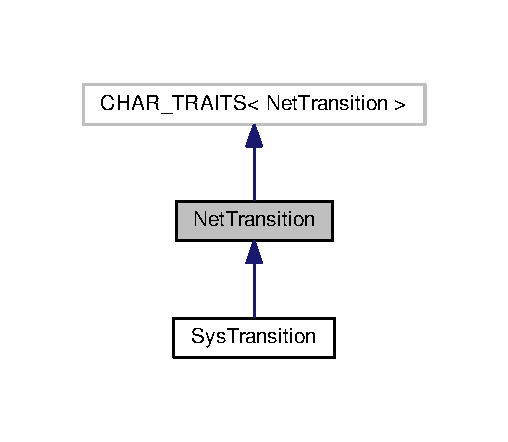
\includegraphics[width=244pt]{class_net_transition__inherit__graph}
\end{center}
\end{figure}


Collaboration diagram for Net\+Transition\+:
\nopagebreak
\begin{figure}[H]
\begin{center}
\leavevmode
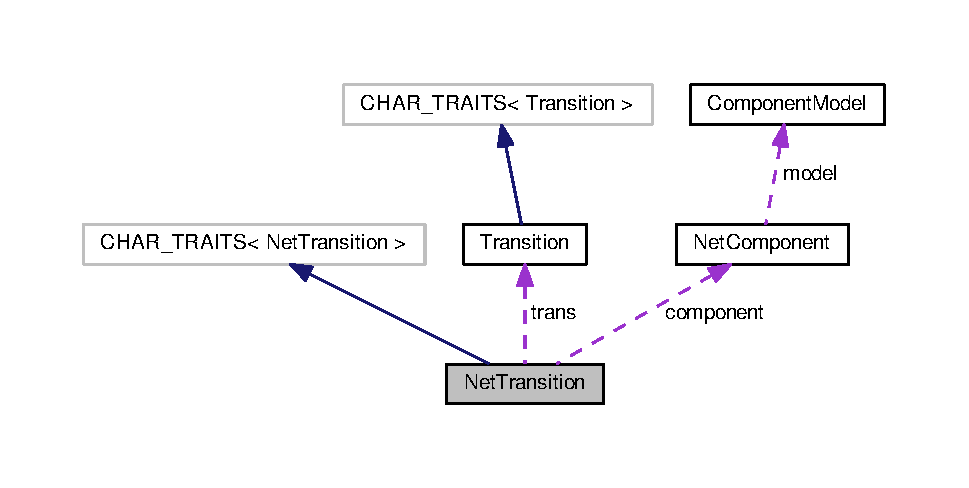
\includegraphics[width=350pt]{class_net_transition__coll__graph}
\end{center}
\end{figure}
\subsection*{Public Types}
\begin{DoxyCompactItemize}
\item 
typedef \hyperlink{class_net_transition}{Net\+Transition} \hyperlink{class_net_transition_a40ad367a5a816d31e7559037c76970f0}{char\+\_\+type}\hypertarget{class_net_transition_a40ad367a5a816d31e7559037c76970f0}{}\label{class_net_transition_a40ad367a5a816d31e7559037c76970f0}

\begin{DoxyCompactList}\small\item\em char\+\_\+type \end{DoxyCompactList}\item 
typedef long \hyperlink{class_net_transition_a0f9d17d0e4e371ec89c6c2f4bccd1a63}{int\+\_\+type}\hypertarget{class_net_transition_a0f9d17d0e4e371ec89c6c2f4bccd1a63}{}\label{class_net_transition_a0f9d17d0e4e371ec89c6c2f4bccd1a63}

\begin{DoxyCompactList}\small\item\em int\+\_\+type \end{DoxyCompactList}\end{DoxyCompactItemize}
\subsection*{Public Member Functions}
\begin{DoxyCompactItemize}
\item 
\hyperlink{class_net_transition_a6d3928f521a06cf6b0220175b05e757a}{Net\+Transition} ()\hypertarget{class_net_transition_a6d3928f521a06cf6b0220175b05e757a}{}\label{class_net_transition_a6d3928f521a06cf6b0220175b05e757a}

\begin{DoxyCompactList}\small\item\em \hyperlink{class_net_transition}{Net\+Transition} default constructor. \end{DoxyCompactList}\item 
\hyperlink{class_net_transition_a958eafdf83fb7cd1dd562a4ac48d668f}{Net\+Transition} (\hyperlink{class_transition}{Transition} $\ast$t, \hyperlink{class_net_component}{Net\+Component} $\ast$c)
\begin{DoxyCompactList}\small\item\em \hyperlink{class_net_transition}{Net\+Transition} constructor from pointers to transition and network component. \end{DoxyCompactList}\item 
std\+::string \hyperlink{class_net_transition_a6058715be2b7de07b7f1be57e5ccb1bb}{get\+\_\+name} () const 
\begin{DoxyCompactList}\small\item\em get\+\_\+name \end{DoxyCompactList}\item 
\hyperlink{class_transition}{Transition} $\ast$ \hyperlink{class_net_transition_ae422d809c42771fab328b22378c80af5}{get\+\_\+trans} () const 
\begin{DoxyCompactList}\small\item\em get\+\_\+trans \end{DoxyCompactList}\item 
\hyperlink{class_net_component}{Net\+Component} $\ast$ \hyperlink{class_net_transition_aa03cb562c3191612bc675172b0b5c90c}{get\+\_\+component} () const 
\begin{DoxyCompactList}\small\item\em get\+\_\+component \end{DoxyCompactList}\item 
bool \hyperlink{class_net_transition_ac7d094a518dfdfb784c42702a3db5f9d}{operator$<$} (const \hyperlink{class_net_transition}{Net\+Transition} t) const 
\begin{DoxyCompactList}\small\item\em operator $<$ \end{DoxyCompactList}\item 
bool \hyperlink{class_net_transition_ac7674acf1b41977ebafd99812c648746}{operator==} (const \hyperlink{class_net_transition}{Net\+Transition} t) const 
\begin{DoxyCompactList}\small\item\em operator == \end{DoxyCompactList}\end{DoxyCompactItemize}
\subsection*{Static Public Member Functions}
\begin{DoxyCompactItemize}
\item 
static bool \hyperlink{class_net_transition_a00ab091a8fa7d42fbba4ed634018c5a3}{eq} (const \hyperlink{class_net_transition_a40ad367a5a816d31e7559037c76970f0}{char\+\_\+type} \&x, const \hyperlink{class_net_transition_a40ad367a5a816d31e7559037c76970f0}{char\+\_\+type} \&y)
\begin{DoxyCompactList}\small\item\em eq \end{DoxyCompactList}\item 
static bool \hyperlink{class_net_transition_a30a9ecc563b03dd594afb1077353c1a2}{lt} (const \hyperlink{class_net_transition_a40ad367a5a816d31e7559037c76970f0}{char\+\_\+type} \&x, const \hyperlink{class_net_transition_a40ad367a5a816d31e7559037c76970f0}{char\+\_\+type} \&y)
\begin{DoxyCompactList}\small\item\em lt \end{DoxyCompactList}\end{DoxyCompactItemize}
\subsection*{Static Public Attributes}
\begin{DoxyCompactItemize}
\item 
static const size\+\_\+t \hyperlink{class_net_transition_a1db4742635a4e9d3b6cce5e5669f2ea7}{size}\hypertarget{class_net_transition_a1db4742635a4e9d3b6cce5e5669f2ea7}{}\label{class_net_transition_a1db4742635a4e9d3b6cce5e5669f2ea7}

\begin{DoxyCompactList}\small\item\em size assign value in order to use matrix representation (not specified in this project) \end{DoxyCompactList}\end{DoxyCompactItemize}
\subsection*{Protected Member Functions}
\begin{DoxyCompactItemize}
\item 
{\footnotesize template$<$class Archive $>$ }\\void {\bfseries serialize} (Archive \&ar, const unsigned int version)\hypertarget{class_net_transition_ab6341feb03a31ba89d660a07a94f43e8}{}\label{class_net_transition_ab6341feb03a31ba89d660a07a94f43e8}

\end{DoxyCompactItemize}
\subsection*{Protected Attributes}
\begin{DoxyCompactItemize}
\item 
\hyperlink{class_transition}{Transition} $\ast$ \hyperlink{class_net_transition_ae3b12deb593dab99666592a3686bab9f}{trans}\hypertarget{class_net_transition_ae3b12deb593dab99666592a3686bab9f}{}\label{class_net_transition_ae3b12deb593dab99666592a3686bab9f}

\begin{DoxyCompactList}\small\item\em trans transition of relative component model \end{DoxyCompactList}\item 
\hyperlink{class_net_component}{Net\+Component} $\ast$ \hyperlink{class_net_transition_ac66eef3e787502efbb61baba213b737d}{component}\hypertarget{class_net_transition_ac66eef3e787502efbb61baba213b737d}{}\label{class_net_transition_ac66eef3e787502efbb61baba213b737d}

\begin{DoxyCompactList}\small\item\em component network component involved \end{DoxyCompactList}\item 
std\+::string \hyperlink{class_net_transition_ad2f59243faa110d4a9f887ed791f404d}{name}\hypertarget{class_net_transition_ad2f59243faa110d4a9f887ed791f404d}{}\label{class_net_transition_ad2f59243faa110d4a9f887ed791f404d}

\begin{DoxyCompactList}\small\item\em name \end{DoxyCompactList}\end{DoxyCompactItemize}
\subsection*{Friends}
\begin{DoxyCompactItemize}
\item 
class {\bfseries boost\+::serialization\+::access}\hypertarget{class_net_transition_ac98d07dd8f7b70e16ccb9a01abf56b9c}{}\label{class_net_transition_ac98d07dd8f7b70e16ccb9a01abf56b9c}

\end{DoxyCompactItemize}


\subsection{Detailed Description}
The \hyperlink{class_net_transition}{Net\+Transition} class. 

\begin{DoxyDate}{Date}
Febbraio 2016 
\end{DoxyDate}
\begin{DoxyAuthor}{Author}
Giulio Quarenghi 
\end{DoxyAuthor}


\subsection{Constructor \& Destructor Documentation}
\index{Net\+Transition@{Net\+Transition}!Net\+Transition@{Net\+Transition}}
\index{Net\+Transition@{Net\+Transition}!Net\+Transition@{Net\+Transition}}
\subsubsection[{\texorpdfstring{Net\+Transition(\+Transition $\ast$t, Net\+Component $\ast$c)}{NetTransition(Transition *t, NetComponent *c)}}]{\setlength{\rightskip}{0pt plus 5cm}Net\+Transition\+::\+Net\+Transition (
\begin{DoxyParamCaption}
\item[{{\bf Transition} $\ast$}]{t, }
\item[{{\bf Net\+Component} $\ast$}]{c}
\end{DoxyParamCaption}
)}\hypertarget{class_net_transition_a958eafdf83fb7cd1dd562a4ac48d668f}{}\label{class_net_transition_a958eafdf83fb7cd1dd562a4ac48d668f}


\hyperlink{class_net_transition}{Net\+Transition} constructor from pointers to transition and network component. 


\begin{DoxyParams}{Parameters}
{\em t} & \\
\hline
{\em c} & \\
\hline
\end{DoxyParams}


\subsection{Member Function Documentation}
\index{Net\+Transition@{Net\+Transition}!eq@{eq}}
\index{eq@{eq}!Net\+Transition@{Net\+Transition}}
\subsubsection[{\texorpdfstring{eq(const char\+\_\+type \&x, const char\+\_\+type \&y)}{eq(const char_type &x, const char_type &y)}}]{\setlength{\rightskip}{0pt plus 5cm}static bool Net\+Transition\+::eq (
\begin{DoxyParamCaption}
\item[{const {\bf char\+\_\+type} \&}]{x, }
\item[{const {\bf char\+\_\+type} \&}]{y}
\end{DoxyParamCaption}
)\hspace{0.3cm}{\ttfamily [inline]}, {\ttfamily [static]}}\hypertarget{class_net_transition_a00ab091a8fa7d42fbba4ed634018c5a3}{}\label{class_net_transition_a00ab091a8fa7d42fbba4ed634018c5a3}


eq 


\begin{DoxyParams}{Parameters}
{\em x} & \\
\hline
{\em y} & \\
\hline
\end{DoxyParams}
\begin{DoxyReturn}{Returns}

\end{DoxyReturn}
\index{Net\+Transition@{Net\+Transition}!get\+\_\+component@{get\+\_\+component}}
\index{get\+\_\+component@{get\+\_\+component}!Net\+Transition@{Net\+Transition}}
\subsubsection[{\texorpdfstring{get\+\_\+component() const }{get_component() const }}]{\setlength{\rightskip}{0pt plus 5cm}{\bf Net\+Component} $\ast$ Net\+Transition\+::get\+\_\+component (
\begin{DoxyParamCaption}
{}
\end{DoxyParamCaption}
) const}\hypertarget{class_net_transition_aa03cb562c3191612bc675172b0b5c90c}{}\label{class_net_transition_aa03cb562c3191612bc675172b0b5c90c}


get\+\_\+component 

\begin{DoxyReturn}{Returns}

\end{DoxyReturn}
\index{Net\+Transition@{Net\+Transition}!get\+\_\+name@{get\+\_\+name}}
\index{get\+\_\+name@{get\+\_\+name}!Net\+Transition@{Net\+Transition}}
\subsubsection[{\texorpdfstring{get\+\_\+name() const }{get_name() const }}]{\setlength{\rightskip}{0pt plus 5cm}std\+::string Net\+Transition\+::get\+\_\+name (
\begin{DoxyParamCaption}
{}
\end{DoxyParamCaption}
) const}\hypertarget{class_net_transition_a6058715be2b7de07b7f1be57e5ccb1bb}{}\label{class_net_transition_a6058715be2b7de07b7f1be57e5ccb1bb}


get\+\_\+name 

\begin{DoxyReturn}{Returns}

\end{DoxyReturn}
\index{Net\+Transition@{Net\+Transition}!get\+\_\+trans@{get\+\_\+trans}}
\index{get\+\_\+trans@{get\+\_\+trans}!Net\+Transition@{Net\+Transition}}
\subsubsection[{\texorpdfstring{get\+\_\+trans() const }{get_trans() const }}]{\setlength{\rightskip}{0pt plus 5cm}{\bf Transition} $\ast$ Net\+Transition\+::get\+\_\+trans (
\begin{DoxyParamCaption}
{}
\end{DoxyParamCaption}
) const}\hypertarget{class_net_transition_ae422d809c42771fab328b22378c80af5}{}\label{class_net_transition_ae422d809c42771fab328b22378c80af5}


get\+\_\+trans 

\begin{DoxyReturn}{Returns}

\end{DoxyReturn}
\index{Net\+Transition@{Net\+Transition}!lt@{lt}}
\index{lt@{lt}!Net\+Transition@{Net\+Transition}}
\subsubsection[{\texorpdfstring{lt(const char\+\_\+type \&x, const char\+\_\+type \&y)}{lt(const char_type &x, const char_type &y)}}]{\setlength{\rightskip}{0pt plus 5cm}static bool Net\+Transition\+::lt (
\begin{DoxyParamCaption}
\item[{const {\bf char\+\_\+type} \&}]{x, }
\item[{const {\bf char\+\_\+type} \&}]{y}
\end{DoxyParamCaption}
)\hspace{0.3cm}{\ttfamily [inline]}, {\ttfamily [static]}}\hypertarget{class_net_transition_a30a9ecc563b03dd594afb1077353c1a2}{}\label{class_net_transition_a30a9ecc563b03dd594afb1077353c1a2}


lt 


\begin{DoxyParams}{Parameters}
{\em x} & \\
\hline
{\em y} & \\
\hline
\end{DoxyParams}
\begin{DoxyReturn}{Returns}

\end{DoxyReturn}
\index{Net\+Transition@{Net\+Transition}!operator$<$@{operator$<$}}
\index{operator$<$@{operator$<$}!Net\+Transition@{Net\+Transition}}
\subsubsection[{\texorpdfstring{operator$<$(const Net\+Transition t) const }{operator<(const NetTransition t) const }}]{\setlength{\rightskip}{0pt plus 5cm}bool Net\+Transition\+::operator$<$ (
\begin{DoxyParamCaption}
\item[{const {\bf Net\+Transition}}]{t}
\end{DoxyParamCaption}
) const\hspace{0.3cm}{\ttfamily [inline]}}\hypertarget{class_net_transition_ac7d094a518dfdfb784c42702a3db5f9d}{}\label{class_net_transition_ac7d094a518dfdfb784c42702a3db5f9d}


operator $<$ 


\begin{DoxyParams}{Parameters}
{\em t} & \\
\hline
\end{DoxyParams}
\begin{DoxyReturn}{Returns}

\end{DoxyReturn}
\index{Net\+Transition@{Net\+Transition}!operator==@{operator==}}
\index{operator==@{operator==}!Net\+Transition@{Net\+Transition}}
\subsubsection[{\texorpdfstring{operator==(const Net\+Transition t) const }{operator==(const NetTransition t) const }}]{\setlength{\rightskip}{0pt plus 5cm}bool Net\+Transition\+::operator== (
\begin{DoxyParamCaption}
\item[{const {\bf Net\+Transition}}]{t}
\end{DoxyParamCaption}
) const\hspace{0.3cm}{\ttfamily [inline]}}\hypertarget{class_net_transition_ac7674acf1b41977ebafd99812c648746}{}\label{class_net_transition_ac7674acf1b41977ebafd99812c648746}


operator == 


\begin{DoxyParams}{Parameters}
{\em t} & \\
\hline
\end{DoxyParams}
\begin{DoxyReturn}{Returns}

\end{DoxyReturn}


The documentation for this class was generated from the following files\+:\begin{DoxyCompactItemize}
\item 
nettransition.\+h\item 
nettransition.\+cpp\end{DoxyCompactItemize}

\hypertarget{class_network_model}{}\section{Network\+Model Class Reference}
\label{class_network_model}\index{Network\+Model@{Network\+Model}}


The \hyperlink{class_network_model}{Network\+Model} class.  




{\ttfamily \#include $<$networkmodel.\+h$>$}

\subsection*{Public Member Functions}
\begin{DoxyCompactItemize}
\item 
\hyperlink{class_network_model_a680923e0ff3293e1ac1853c5bfff6626}{Network\+Model} ()\hypertarget{class_network_model_a680923e0ff3293e1ac1853c5bfff6626}{}\label{class_network_model_a680923e0ff3293e1ac1853c5bfff6626}

\begin{DoxyCompactList}\small\item\em \hyperlink{class_network_model}{Network\+Model} default constructor. \end{DoxyCompactList}\item 
\hyperlink{class_network_model_aa9163a8897dc4b0961d6b283fafb243d}{Network\+Model} (std\+::string str)
\begin{DoxyCompactList}\small\item\em \hyperlink{class_network_model}{Network\+Model} constructor from id. \end{DoxyCompactList}\item 
std\+::string \hyperlink{class_network_model_ade7b5e15e745b08ae6d5f13e0447ab20}{get\+\_\+name} () const 
\begin{DoxyCompactList}\small\item\em get\+\_\+name \end{DoxyCompactList}\item 
vector$<$ \hyperlink{class_net_component}{Net\+Component} $>$ \hyperlink{class_network_model_abce681ce925e7d379091932650177af3}{get\+\_\+components} () const 
\begin{DoxyCompactList}\small\item\em get\+\_\+components \end{DoxyCompactList}\item 
vector$<$ std\+::string $>$ \hyperlink{class_network_model_ad0f615741e4cf35edbdd0e1325b261f6}{get\+\_\+inputs} () const 
\begin{DoxyCompactList}\small\item\em get\+\_\+inputs \end{DoxyCompactList}\item 
vector$<$ std\+::string $>$ \hyperlink{class_network_model_aa26c3852306f0861ac86a312a3de0cc7}{get\+\_\+outputs} () const 
\begin{DoxyCompactList}\small\item\em get\+\_\+outputs \end{DoxyCompactList}\item 
vector$<$ pair$<$ pair$<$ std\+::string, std\+::string $>$, pair$<$ std\+::string, std\+::string $>$ $>$ $>$ \hyperlink{class_network_model_a83a9cf2752510f7a8d76cb6f91cf5c6a}{get\+\_\+links} () const 
\begin{DoxyCompactList}\small\item\em get\+\_\+links \end{DoxyCompactList}\item 
vector$<$ \hyperlink{class_pattern}{Pattern} $>$ \hyperlink{class_network_model_af72c9c9d6889647c091786fefdb184a9}{get\+\_\+patterns} () const 
\begin{DoxyCompactList}\small\item\em get\+\_\+patterns \end{DoxyCompactList}\item 
vector$<$ pair$<$ std\+::string, std\+::string $>$ $>$ \hyperlink{class_network_model_a6e227573863655c96aa1b6cf7136863a}{get\+\_\+initials} () const 
\begin{DoxyCompactList}\small\item\em get\+\_\+initials \end{DoxyCompactList}\item 
map$<$ pair$<$ string, string $>$, string $>$ \hyperlink{class_network_model_ac1546106a62f35dca850f23a2c137c9b}{get\+\_\+viewer} () const 
\begin{DoxyCompactList}\small\item\em get\+\_\+viewer \end{DoxyCompactList}\item 
map$<$ pair$<$ string, string $>$, string $>$ \hyperlink{class_network_model_a8aebf68fbb04f19840641c4e12540d13}{get\+\_\+ruler} () const 
\begin{DoxyCompactList}\small\item\em get\+\_\+ruler \end{DoxyCompactList}\item 
vector$<$ astl\+::\+D\+F\+A\+\_\+map$<$ \hyperlink{class_net_transition}{Net\+Transition}, \hyperlink{class_state_data__str_list}{State\+Data\+\_\+str\+List} $>$ $\ast$ $>$ \hyperlink{class_network_model_ae34c23f6543d3cb4a5c1ef5ae18ac1a0}{get\+\_\+pattern\+\_\+space} () const 
\begin{DoxyCompactList}\small\item\em get\+\_\+pattern\+\_\+space \end{DoxyCompactList}\item 
vector$<$ set$<$ string $>$ $>$ \hyperlink{class_network_model_aee2158178eb05711c5f438f365bbe959}{get\+\_\+pattern\+\_\+languages} () const 
\begin{DoxyCompactList}\small\item\em get\+\_\+pattern\+\_\+languages \end{DoxyCompactList}\item 
void \hyperlink{class_network_model_adb9a3df843ce10b846f1a6d42d36ab89}{add\+\_\+comp} (\hyperlink{class_net_component}{Net\+Component} nc)
\begin{DoxyCompactList}\small\item\em add\+\_\+comp \end{DoxyCompactList}\item 
void \hyperlink{class_network_model_a8abdad23ae7632e76df54c7ba69f49bc}{add\+\_\+input} (std\+::string in)
\begin{DoxyCompactList}\small\item\em add\+\_\+input \end{DoxyCompactList}\item 
void \hyperlink{class_network_model_aad3bec0b61c3b3b7e8fbaa3f03d1ae45}{add\+\_\+output} (std\+::string out)
\begin{DoxyCompactList}\small\item\em add\+\_\+output \end{DoxyCompactList}\item 
void \hyperlink{class_network_model_aa5b933f3e3874d655aa5e9c81bff76bc}{add\+\_\+link} (std\+::string t1, std\+::string c1, std\+::string t2, std\+::string c2)
\begin{DoxyCompactList}\small\item\em add\+\_\+link \end{DoxyCompactList}\item 
void \hyperlink{class_network_model_a8c43ca2b56e307410d8dad56392ce773}{add\+\_\+pattern} (\hyperlink{class_pattern}{Pattern} p)
\begin{DoxyCompactList}\small\item\em add\+\_\+pattern \end{DoxyCompactList}\item 
void \hyperlink{class_network_model_a4e76c93d40e4b3e890d07b6bbda11028}{add\+\_\+initial} (std\+::string state, std\+::string c)
\begin{DoxyCompactList}\small\item\em add\+\_\+initial \end{DoxyCompactList}\item 
void \hyperlink{class_network_model_ad3aa91bba2f26afb2cc2a25f29897420}{add\+\_\+label} (pair$<$ string, string $>$ t, std\+::string l)
\begin{DoxyCompactList}\small\item\em add\+\_\+label \end{DoxyCompactList}\item 
void \hyperlink{class_network_model_a08043ed822076e4a9919c9778093cd12}{add\+\_\+fault} (pair$<$ string, string $>$ t, std\+::string f)
\begin{DoxyCompactList}\small\item\em add\+\_\+fault \end{DoxyCompactList}\item 
void \hyperlink{class_network_model_a3eb4abcd7feb1c3679fc774c217e28a8}{add\+\_\+pattern\+\_\+space} (astl\+::\+D\+F\+A\+\_\+map$<$ \hyperlink{class_net_transition}{Net\+Transition}, \hyperlink{class_state_data__str_list}{State\+Data\+\_\+str\+List} $>$ $\ast$pts)
\begin{DoxyCompactList}\small\item\em add\+\_\+pattern\+\_\+space \end{DoxyCompactList}\item 
void \hyperlink{class_network_model_a019437545f5aeb663e72bc228c287e29}{add\+\_\+language} (set$<$ std\+::string $>$ l)
\begin{DoxyCompactList}\small\item\em add\+\_\+language \end{DoxyCompactList}\item 
void \hyperlink{class_network_model_a8f6e2ed529313d9e88fe8e2069a748f7}{set\+\_\+components} (vector$<$ \hyperlink{class_net_component}{Net\+Component} $>$ vc)
\begin{DoxyCompactList}\small\item\em set\+\_\+components \end{DoxyCompactList}\item 
void \hyperlink{class_network_model_a971e36a67cebd56453a72692f4be7f6e}{set\+\_\+inputs} (vector$<$ std\+::string $>$ vi)
\begin{DoxyCompactList}\small\item\em set\+\_\+inputs \end{DoxyCompactList}\item 
void \hyperlink{class_network_model_a91d15b0367a25661db90c51adaec4302}{set\+\_\+outputs} (vector$<$ std\+::string $>$ vo)
\begin{DoxyCompactList}\small\item\em set\+\_\+outputs \end{DoxyCompactList}\item 
void \hyperlink{class_network_model_a0669f9fc1a612585a6e1977666928557}{set\+\_\+links} (vector$<$ pair$<$ pair$<$ std\+::string, std\+::string $>$, pair$<$ std\+::string, std\+::string $>$ $>$ $>$ vl)
\begin{DoxyCompactList}\small\item\em set\+\_\+links \end{DoxyCompactList}\item 
void \hyperlink{class_network_model_a8efd039e281fc53492661b3f595c2c8c}{set\+\_\+patterns} (vector$<$ \hyperlink{class_pattern}{Pattern} $>$ vp)
\begin{DoxyCompactList}\small\item\em set\+\_\+patterns \end{DoxyCompactList}\item 
void \hyperlink{class_network_model_abd3d5fb2d8fa7f4d7337101d017ad7cc}{set\+\_\+initials} (vector$<$ pair$<$ std\+::string, std\+::string $>$ $>$ vi)
\begin{DoxyCompactList}\small\item\em set\+\_\+initials \end{DoxyCompactList}\item 
void \hyperlink{class_network_model_a0ab949112040285f3dccbef024562c88}{set\+\_\+viewer} (map$<$ pair$<$ string, string $>$, string $>$ vwr)
\begin{DoxyCompactList}\small\item\em set\+\_\+viewer \end{DoxyCompactList}\item 
void \hyperlink{class_network_model_a22f2b04c55a7e8ea7d48bc392c7874b3}{set\+\_\+ruler} (map$<$ pair$<$ string, string $>$, string $>$ rlr)
\begin{DoxyCompactList}\small\item\em set\+\_\+ruler \end{DoxyCompactList}\item 
std\+::string \hyperlink{class_network_model_a0cdc08acf73010472700db9d690eb4d2}{not\+\_\+trans} (std\+::string operand)
\begin{DoxyCompactList}\small\item\em not\+\_\+trans computes not operation on regular expressions \end{DoxyCompactList}\item 
\hyperlink{class_net_component}{Net\+Component} $\ast$ \hyperlink{class_network_model_ab2edbaffc9e90c754cbb3ac5b515d74f}{find\+\_\+component} (std\+::string id)
\begin{DoxyCompactList}\small\item\em find\+\_\+component from id \end{DoxyCompactList}\end{DoxyCompactItemize}
\subsection*{Public Attributes}
\begin{DoxyCompactItemize}
\item 
int {\bfseries count}\hypertarget{class_network_model_a82ec303222e3a0207865dfb6ed3b81ff}{}\label{class_network_model_a82ec303222e3a0207865dfb6ed3b81ff}

\item 
std\+::map$<$ std\+::pair$<$ std\+::string, std\+::string $>$, int $>$ \hyperlink{class_network_model_a826def67a5afb8534a1a32c7a8eba84a}{conv\+\_\+str\+\_\+int}\hypertarget{class_network_model_a826def67a5afb8534a1a32c7a8eba84a}{}\label{class_network_model_a826def67a5afb8534a1a32c7a8eba84a}

\begin{DoxyCompactList}\small\item\em conv\+\_\+str\+\_\+int maps transition into number \end{DoxyCompactList}\item 
std\+::map$<$ int, std\+::pair$<$ std\+::string, std\+::string $>$ $>$ \hyperlink{class_network_model_af008577d60bc685e58c181b85142eccf}{conv\+\_\+int\+\_\+str}\hypertarget{class_network_model_af008577d60bc685e58c181b85142eccf}{}\label{class_network_model_af008577d60bc685e58c181b85142eccf}

\begin{DoxyCompactList}\small\item\em conv\+\_\+int\+\_\+str maps number into transition \end{DoxyCompactList}\end{DoxyCompactItemize}
\subsection*{Friends}
\begin{DoxyCompactItemize}
\item 
class {\bfseries boost\+::serialization\+::access}\hypertarget{class_network_model_ac98d07dd8f7b70e16ccb9a01abf56b9c}{}\label{class_network_model_ac98d07dd8f7b70e16ccb9a01abf56b9c}

\end{DoxyCompactItemize}


\subsection{Detailed Description}
The \hyperlink{class_network_model}{Network\+Model} class. 

\begin{DoxyDate}{Date}
Febbraio 2016 
\end{DoxyDate}
\begin{DoxyAuthor}{Author}
Giulio Quarenghi 
\end{DoxyAuthor}


\subsection{Constructor \& Destructor Documentation}
\index{Network\+Model@{Network\+Model}!Network\+Model@{Network\+Model}}
\index{Network\+Model@{Network\+Model}!Network\+Model@{Network\+Model}}
\subsubsection[{\texorpdfstring{Network\+Model(std\+::string str)}{NetworkModel(std::string str)}}]{\setlength{\rightskip}{0pt plus 5cm}Network\+Model\+::\+Network\+Model (
\begin{DoxyParamCaption}
\item[{std\+::string}]{str}
\end{DoxyParamCaption}
)}\hypertarget{class_network_model_aa9163a8897dc4b0961d6b283fafb243d}{}\label{class_network_model_aa9163a8897dc4b0961d6b283fafb243d}


\hyperlink{class_network_model}{Network\+Model} constructor from id. 


\begin{DoxyParams}{Parameters}
{\em str} & name \\
\hline
\end{DoxyParams}


\subsection{Member Function Documentation}
\index{Network\+Model@{Network\+Model}!add\+\_\+comp@{add\+\_\+comp}}
\index{add\+\_\+comp@{add\+\_\+comp}!Network\+Model@{Network\+Model}}
\subsubsection[{\texorpdfstring{add\+\_\+comp(\+Net\+Component nc)}{add_comp(NetComponent nc)}}]{\setlength{\rightskip}{0pt plus 5cm}void Network\+Model\+::add\+\_\+comp (
\begin{DoxyParamCaption}
\item[{{\bf Net\+Component}}]{nc}
\end{DoxyParamCaption}
)}\hypertarget{class_network_model_adb9a3df843ce10b846f1a6d42d36ab89}{}\label{class_network_model_adb9a3df843ce10b846f1a6d42d36ab89}


add\+\_\+comp 


\begin{DoxyParams}{Parameters}
{\em nc} & \\
\hline
\end{DoxyParams}
\index{Network\+Model@{Network\+Model}!add\+\_\+fault@{add\+\_\+fault}}
\index{add\+\_\+fault@{add\+\_\+fault}!Network\+Model@{Network\+Model}}
\subsubsection[{\texorpdfstring{add\+\_\+fault(pair$<$ string, string $>$ t, std\+::string f)}{add_fault(pair< string, string > t, std::string f)}}]{\setlength{\rightskip}{0pt plus 5cm}void Network\+Model\+::add\+\_\+fault (
\begin{DoxyParamCaption}
\item[{pair$<$ string, string $>$}]{t, }
\item[{std\+::string}]{f}
\end{DoxyParamCaption}
)}\hypertarget{class_network_model_a08043ed822076e4a9919c9778093cd12}{}\label{class_network_model_a08043ed822076e4a9919c9778093cd12}


add\+\_\+fault 


\begin{DoxyParams}{Parameters}
{\em t} & \\
\hline
{\em f} & \\
\hline
\end{DoxyParams}
\index{Network\+Model@{Network\+Model}!add\+\_\+initial@{add\+\_\+initial}}
\index{add\+\_\+initial@{add\+\_\+initial}!Network\+Model@{Network\+Model}}
\subsubsection[{\texorpdfstring{add\+\_\+initial(std\+::string state, std\+::string c)}{add_initial(std::string state, std::string c)}}]{\setlength{\rightskip}{0pt plus 5cm}void Network\+Model\+::add\+\_\+initial (
\begin{DoxyParamCaption}
\item[{std\+::string}]{state, }
\item[{std\+::string}]{c}
\end{DoxyParamCaption}
)}\hypertarget{class_network_model_a4e76c93d40e4b3e890d07b6bbda11028}{}\label{class_network_model_a4e76c93d40e4b3e890d07b6bbda11028}


add\+\_\+initial 


\begin{DoxyParams}{Parameters}
{\em state} & \\
\hline
{\em c} & \\
\hline
\end{DoxyParams}
\index{Network\+Model@{Network\+Model}!add\+\_\+input@{add\+\_\+input}}
\index{add\+\_\+input@{add\+\_\+input}!Network\+Model@{Network\+Model}}
\subsubsection[{\texorpdfstring{add\+\_\+input(std\+::string in)}{add_input(std::string in)}}]{\setlength{\rightskip}{0pt plus 5cm}void Network\+Model\+::add\+\_\+input (
\begin{DoxyParamCaption}
\item[{std\+::string}]{in}
\end{DoxyParamCaption}
)}\hypertarget{class_network_model_a8abdad23ae7632e76df54c7ba69f49bc}{}\label{class_network_model_a8abdad23ae7632e76df54c7ba69f49bc}


add\+\_\+input 


\begin{DoxyParams}{Parameters}
{\em in} & \\
\hline
\end{DoxyParams}
\index{Network\+Model@{Network\+Model}!add\+\_\+label@{add\+\_\+label}}
\index{add\+\_\+label@{add\+\_\+label}!Network\+Model@{Network\+Model}}
\subsubsection[{\texorpdfstring{add\+\_\+label(pair$<$ string, string $>$ t, std\+::string l)}{add_label(pair< string, string > t, std::string l)}}]{\setlength{\rightskip}{0pt plus 5cm}void Network\+Model\+::add\+\_\+label (
\begin{DoxyParamCaption}
\item[{pair$<$ string, string $>$}]{t, }
\item[{std\+::string}]{l}
\end{DoxyParamCaption}
)}\hypertarget{class_network_model_ad3aa91bba2f26afb2cc2a25f29897420}{}\label{class_network_model_ad3aa91bba2f26afb2cc2a25f29897420}


add\+\_\+label 


\begin{DoxyParams}{Parameters}
{\em t} & \\
\hline
{\em l} & \\
\hline
\end{DoxyParams}
\index{Network\+Model@{Network\+Model}!add\+\_\+language@{add\+\_\+language}}
\index{add\+\_\+language@{add\+\_\+language}!Network\+Model@{Network\+Model}}
\subsubsection[{\texorpdfstring{add\+\_\+language(set$<$ std\+::string $>$ l)}{add_language(set< std::string > l)}}]{\setlength{\rightskip}{0pt plus 5cm}void Network\+Model\+::add\+\_\+language (
\begin{DoxyParamCaption}
\item[{set$<$ std\+::string $>$}]{l}
\end{DoxyParamCaption}
)}\hypertarget{class_network_model_a019437545f5aeb663e72bc228c287e29}{}\label{class_network_model_a019437545f5aeb663e72bc228c287e29}


add\+\_\+language 


\begin{DoxyParams}{Parameters}
{\em l} & \\
\hline
\end{DoxyParams}
\index{Network\+Model@{Network\+Model}!add\+\_\+link@{add\+\_\+link}}
\index{add\+\_\+link@{add\+\_\+link}!Network\+Model@{Network\+Model}}
\subsubsection[{\texorpdfstring{add\+\_\+link(std\+::string t1, std\+::string c1, std\+::string t2, std\+::string c2)}{add_link(std::string t1, std::string c1, std::string t2, std::string c2)}}]{\setlength{\rightskip}{0pt plus 5cm}void Network\+Model\+::add\+\_\+link (
\begin{DoxyParamCaption}
\item[{std\+::string}]{t1, }
\item[{std\+::string}]{c1, }
\item[{std\+::string}]{t2, }
\item[{std\+::string}]{c2}
\end{DoxyParamCaption}
)}\hypertarget{class_network_model_aa5b933f3e3874d655aa5e9c81bff76bc}{}\label{class_network_model_aa5b933f3e3874d655aa5e9c81bff76bc}


add\+\_\+link 


\begin{DoxyParams}{Parameters}
{\em t1} & \\
\hline
{\em c1} & \\
\hline
{\em t2} & \\
\hline
{\em c2} & \\
\hline
\end{DoxyParams}
\index{Network\+Model@{Network\+Model}!add\+\_\+output@{add\+\_\+output}}
\index{add\+\_\+output@{add\+\_\+output}!Network\+Model@{Network\+Model}}
\subsubsection[{\texorpdfstring{add\+\_\+output(std\+::string out)}{add_output(std::string out)}}]{\setlength{\rightskip}{0pt plus 5cm}void Network\+Model\+::add\+\_\+output (
\begin{DoxyParamCaption}
\item[{std\+::string}]{out}
\end{DoxyParamCaption}
)}\hypertarget{class_network_model_aad3bec0b61c3b3b7e8fbaa3f03d1ae45}{}\label{class_network_model_aad3bec0b61c3b3b7e8fbaa3f03d1ae45}


add\+\_\+output 


\begin{DoxyParams}{Parameters}
{\em out} & \\
\hline
\end{DoxyParams}
\index{Network\+Model@{Network\+Model}!add\+\_\+pattern@{add\+\_\+pattern}}
\index{add\+\_\+pattern@{add\+\_\+pattern}!Network\+Model@{Network\+Model}}
\subsubsection[{\texorpdfstring{add\+\_\+pattern(\+Pattern p)}{add_pattern(Pattern p)}}]{\setlength{\rightskip}{0pt plus 5cm}void Network\+Model\+::add\+\_\+pattern (
\begin{DoxyParamCaption}
\item[{{\bf Pattern}}]{p}
\end{DoxyParamCaption}
)}\hypertarget{class_network_model_a8c43ca2b56e307410d8dad56392ce773}{}\label{class_network_model_a8c43ca2b56e307410d8dad56392ce773}


add\+\_\+pattern 


\begin{DoxyParams}{Parameters}
{\em p} & \\
\hline
\end{DoxyParams}
\index{Network\+Model@{Network\+Model}!add\+\_\+pattern\+\_\+space@{add\+\_\+pattern\+\_\+space}}
\index{add\+\_\+pattern\+\_\+space@{add\+\_\+pattern\+\_\+space}!Network\+Model@{Network\+Model}}
\subsubsection[{\texorpdfstring{add\+\_\+pattern\+\_\+space(astl\+::\+D\+F\+A\+\_\+map$<$ Net\+Transition, State\+Data\+\_\+str\+List $>$ $\ast$pts)}{add_pattern_space(astl::DFA_map< NetTransition, StateData_strList > *pts)}}]{\setlength{\rightskip}{0pt plus 5cm}void Network\+Model\+::add\+\_\+pattern\+\_\+space (
\begin{DoxyParamCaption}
\item[{astl\+::\+D\+F\+A\+\_\+map$<$ {\bf Net\+Transition}, {\bf State\+Data\+\_\+str\+List} $>$ $\ast$}]{pts}
\end{DoxyParamCaption}
)}\hypertarget{class_network_model_a3eb4abcd7feb1c3679fc774c217e28a8}{}\label{class_network_model_a3eb4abcd7feb1c3679fc774c217e28a8}


add\+\_\+pattern\+\_\+space 


\begin{DoxyParams}{Parameters}
{\em pts} & \\
\hline
\end{DoxyParams}
\index{Network\+Model@{Network\+Model}!find\+\_\+component@{find\+\_\+component}}
\index{find\+\_\+component@{find\+\_\+component}!Network\+Model@{Network\+Model}}
\subsubsection[{\texorpdfstring{find\+\_\+component(std\+::string id)}{find_component(std::string id)}}]{\setlength{\rightskip}{0pt plus 5cm}{\bf Net\+Component} $\ast$ Network\+Model\+::find\+\_\+component (
\begin{DoxyParamCaption}
\item[{std\+::string}]{id}
\end{DoxyParamCaption}
)}\hypertarget{class_network_model_ab2edbaffc9e90c754cbb3ac5b515d74f}{}\label{class_network_model_ab2edbaffc9e90c754cbb3ac5b515d74f}


find\+\_\+component from id 


\begin{DoxyParams}{Parameters}
{\em id} & \\
\hline
\end{DoxyParams}
\begin{DoxyReturn}{Returns}
pointer to \hyperlink{class_net_component}{Net\+Component} 
\end{DoxyReturn}
\index{Network\+Model@{Network\+Model}!get\+\_\+components@{get\+\_\+components}}
\index{get\+\_\+components@{get\+\_\+components}!Network\+Model@{Network\+Model}}
\subsubsection[{\texorpdfstring{get\+\_\+components() const }{get_components() const }}]{\setlength{\rightskip}{0pt plus 5cm}vector$<$ {\bf Net\+Component} $>$ Network\+Model\+::get\+\_\+components (
\begin{DoxyParamCaption}
{}
\end{DoxyParamCaption}
) const}\hypertarget{class_network_model_abce681ce925e7d379091932650177af3}{}\label{class_network_model_abce681ce925e7d379091932650177af3}


get\+\_\+components 

\begin{DoxyReturn}{Returns}

\end{DoxyReturn}
\index{Network\+Model@{Network\+Model}!get\+\_\+initials@{get\+\_\+initials}}
\index{get\+\_\+initials@{get\+\_\+initials}!Network\+Model@{Network\+Model}}
\subsubsection[{\texorpdfstring{get\+\_\+initials() const }{get_initials() const }}]{\setlength{\rightskip}{0pt plus 5cm}vector$<$ pair$<$ std\+::string, std\+::string $>$ $>$ Network\+Model\+::get\+\_\+initials (
\begin{DoxyParamCaption}
{}
\end{DoxyParamCaption}
) const}\hypertarget{class_network_model_a6e227573863655c96aa1b6cf7136863a}{}\label{class_network_model_a6e227573863655c96aa1b6cf7136863a}


get\+\_\+initials 

\begin{DoxyReturn}{Returns}

\end{DoxyReturn}
\index{Network\+Model@{Network\+Model}!get\+\_\+inputs@{get\+\_\+inputs}}
\index{get\+\_\+inputs@{get\+\_\+inputs}!Network\+Model@{Network\+Model}}
\subsubsection[{\texorpdfstring{get\+\_\+inputs() const }{get_inputs() const }}]{\setlength{\rightskip}{0pt plus 5cm}vector$<$ std\+::string $>$ Network\+Model\+::get\+\_\+inputs (
\begin{DoxyParamCaption}
{}
\end{DoxyParamCaption}
) const}\hypertarget{class_network_model_ad0f615741e4cf35edbdd0e1325b261f6}{}\label{class_network_model_ad0f615741e4cf35edbdd0e1325b261f6}


get\+\_\+inputs 

\begin{DoxyReturn}{Returns}

\end{DoxyReturn}
\index{Network\+Model@{Network\+Model}!get\+\_\+links@{get\+\_\+links}}
\index{get\+\_\+links@{get\+\_\+links}!Network\+Model@{Network\+Model}}
\subsubsection[{\texorpdfstring{get\+\_\+links() const }{get_links() const }}]{\setlength{\rightskip}{0pt plus 5cm}vector$<$ pair$<$ pair$<$ std\+::string, std\+::string $>$, pair$<$ std\+::string, std\+::string $>$ $>$ $>$ Network\+Model\+::get\+\_\+links (
\begin{DoxyParamCaption}
{}
\end{DoxyParamCaption}
) const}\hypertarget{class_network_model_a83a9cf2752510f7a8d76cb6f91cf5c6a}{}\label{class_network_model_a83a9cf2752510f7a8d76cb6f91cf5c6a}


get\+\_\+links 

\begin{DoxyReturn}{Returns}

\end{DoxyReturn}
\index{Network\+Model@{Network\+Model}!get\+\_\+name@{get\+\_\+name}}
\index{get\+\_\+name@{get\+\_\+name}!Network\+Model@{Network\+Model}}
\subsubsection[{\texorpdfstring{get\+\_\+name() const }{get_name() const }}]{\setlength{\rightskip}{0pt plus 5cm}std\+::string Network\+Model\+::get\+\_\+name (
\begin{DoxyParamCaption}
{}
\end{DoxyParamCaption}
) const}\hypertarget{class_network_model_ade7b5e15e745b08ae6d5f13e0447ab20}{}\label{class_network_model_ade7b5e15e745b08ae6d5f13e0447ab20}


get\+\_\+name 

\begin{DoxyReturn}{Returns}

\end{DoxyReturn}
\index{Network\+Model@{Network\+Model}!get\+\_\+outputs@{get\+\_\+outputs}}
\index{get\+\_\+outputs@{get\+\_\+outputs}!Network\+Model@{Network\+Model}}
\subsubsection[{\texorpdfstring{get\+\_\+outputs() const }{get_outputs() const }}]{\setlength{\rightskip}{0pt plus 5cm}vector$<$ std\+::string $>$ Network\+Model\+::get\+\_\+outputs (
\begin{DoxyParamCaption}
{}
\end{DoxyParamCaption}
) const}\hypertarget{class_network_model_aa26c3852306f0861ac86a312a3de0cc7}{}\label{class_network_model_aa26c3852306f0861ac86a312a3de0cc7}


get\+\_\+outputs 

\begin{DoxyReturn}{Returns}

\end{DoxyReturn}
\index{Network\+Model@{Network\+Model}!get\+\_\+pattern\+\_\+languages@{get\+\_\+pattern\+\_\+languages}}
\index{get\+\_\+pattern\+\_\+languages@{get\+\_\+pattern\+\_\+languages}!Network\+Model@{Network\+Model}}
\subsubsection[{\texorpdfstring{get\+\_\+pattern\+\_\+languages() const }{get_pattern_languages() const }}]{\setlength{\rightskip}{0pt plus 5cm}vector$<$ set$<$ string $>$ $>$ Network\+Model\+::get\+\_\+pattern\+\_\+languages (
\begin{DoxyParamCaption}
{}
\end{DoxyParamCaption}
) const}\hypertarget{class_network_model_aee2158178eb05711c5f438f365bbe959}{}\label{class_network_model_aee2158178eb05711c5f438f365bbe959}


get\+\_\+pattern\+\_\+languages 

\begin{DoxyReturn}{Returns}

\end{DoxyReturn}
\index{Network\+Model@{Network\+Model}!get\+\_\+pattern\+\_\+space@{get\+\_\+pattern\+\_\+space}}
\index{get\+\_\+pattern\+\_\+space@{get\+\_\+pattern\+\_\+space}!Network\+Model@{Network\+Model}}
\subsubsection[{\texorpdfstring{get\+\_\+pattern\+\_\+space() const }{get_pattern_space() const }}]{\setlength{\rightskip}{0pt plus 5cm}vector$<$ astl\+::\+D\+F\+A\+\_\+map$<$ {\bf Net\+Transition}, {\bf State\+Data\+\_\+str\+List} $>$ $\ast$ $>$ Network\+Model\+::get\+\_\+pattern\+\_\+space (
\begin{DoxyParamCaption}
{}
\end{DoxyParamCaption}
) const}\hypertarget{class_network_model_ae34c23f6543d3cb4a5c1ef5ae18ac1a0}{}\label{class_network_model_ae34c23f6543d3cb4a5c1ef5ae18ac1a0}


get\+\_\+pattern\+\_\+space 

\begin{DoxyReturn}{Returns}

\end{DoxyReturn}
\index{Network\+Model@{Network\+Model}!get\+\_\+patterns@{get\+\_\+patterns}}
\index{get\+\_\+patterns@{get\+\_\+patterns}!Network\+Model@{Network\+Model}}
\subsubsection[{\texorpdfstring{get\+\_\+patterns() const }{get_patterns() const }}]{\setlength{\rightskip}{0pt plus 5cm}vector$<$ {\bf Pattern} $>$ Network\+Model\+::get\+\_\+patterns (
\begin{DoxyParamCaption}
{}
\end{DoxyParamCaption}
) const}\hypertarget{class_network_model_af72c9c9d6889647c091786fefdb184a9}{}\label{class_network_model_af72c9c9d6889647c091786fefdb184a9}


get\+\_\+patterns 

\begin{DoxyReturn}{Returns}

\end{DoxyReturn}
\index{Network\+Model@{Network\+Model}!get\+\_\+ruler@{get\+\_\+ruler}}
\index{get\+\_\+ruler@{get\+\_\+ruler}!Network\+Model@{Network\+Model}}
\subsubsection[{\texorpdfstring{get\+\_\+ruler() const }{get_ruler() const }}]{\setlength{\rightskip}{0pt plus 5cm}map$<$ pair$<$ string, string $>$, string $>$ Network\+Model\+::get\+\_\+ruler (
\begin{DoxyParamCaption}
{}
\end{DoxyParamCaption}
) const}\hypertarget{class_network_model_a8aebf68fbb04f19840641c4e12540d13}{}\label{class_network_model_a8aebf68fbb04f19840641c4e12540d13}


get\+\_\+ruler 

\begin{DoxyReturn}{Returns}

\end{DoxyReturn}
\index{Network\+Model@{Network\+Model}!get\+\_\+viewer@{get\+\_\+viewer}}
\index{get\+\_\+viewer@{get\+\_\+viewer}!Network\+Model@{Network\+Model}}
\subsubsection[{\texorpdfstring{get\+\_\+viewer() const }{get_viewer() const }}]{\setlength{\rightskip}{0pt plus 5cm}map$<$ pair$<$ string, string $>$, string $>$ Network\+Model\+::get\+\_\+viewer (
\begin{DoxyParamCaption}
{}
\end{DoxyParamCaption}
) const}\hypertarget{class_network_model_ac1546106a62f35dca850f23a2c137c9b}{}\label{class_network_model_ac1546106a62f35dca850f23a2c137c9b}


get\+\_\+viewer 

\begin{DoxyReturn}{Returns}

\end{DoxyReturn}
\index{Network\+Model@{Network\+Model}!not\+\_\+trans@{not\+\_\+trans}}
\index{not\+\_\+trans@{not\+\_\+trans}!Network\+Model@{Network\+Model}}
\subsubsection[{\texorpdfstring{not\+\_\+trans(std\+::string operand)}{not_trans(std::string operand)}}]{\setlength{\rightskip}{0pt plus 5cm}std\+::string Network\+Model\+::not\+\_\+trans (
\begin{DoxyParamCaption}
\item[{std\+::string}]{operand}
\end{DoxyParamCaption}
)}\hypertarget{class_network_model_a0cdc08acf73010472700db9d690eb4d2}{}\label{class_network_model_a0cdc08acf73010472700db9d690eb4d2}


not\+\_\+trans computes not operation on regular expressions 


\begin{DoxyParams}{Parameters}
{\em operand} & \\
\hline
\end{DoxyParams}
\begin{DoxyReturn}{Returns}

\end{DoxyReturn}
\index{Network\+Model@{Network\+Model}!set\+\_\+components@{set\+\_\+components}}
\index{set\+\_\+components@{set\+\_\+components}!Network\+Model@{Network\+Model}}
\subsubsection[{\texorpdfstring{set\+\_\+components(vector$<$ Net\+Component $>$ vc)}{set_components(vector< NetComponent > vc)}}]{\setlength{\rightskip}{0pt plus 5cm}void Network\+Model\+::set\+\_\+components (
\begin{DoxyParamCaption}
\item[{vector$<$ {\bf Net\+Component} $>$}]{vc}
\end{DoxyParamCaption}
)}\hypertarget{class_network_model_a8f6e2ed529313d9e88fe8e2069a748f7}{}\label{class_network_model_a8f6e2ed529313d9e88fe8e2069a748f7}


set\+\_\+components 


\begin{DoxyParams}{Parameters}
{\em vc} & \\
\hline
\end{DoxyParams}
\index{Network\+Model@{Network\+Model}!set\+\_\+initials@{set\+\_\+initials}}
\index{set\+\_\+initials@{set\+\_\+initials}!Network\+Model@{Network\+Model}}
\subsubsection[{\texorpdfstring{set\+\_\+initials(vector$<$ pair$<$ std\+::string, std\+::string $>$ $>$ vi)}{set_initials(vector< pair< std::string, std::string > > vi)}}]{\setlength{\rightskip}{0pt plus 5cm}void Network\+Model\+::set\+\_\+initials (
\begin{DoxyParamCaption}
\item[{vector$<$ pair$<$ std\+::string, std\+::string $>$ $>$}]{vi}
\end{DoxyParamCaption}
)}\hypertarget{class_network_model_abd3d5fb2d8fa7f4d7337101d017ad7cc}{}\label{class_network_model_abd3d5fb2d8fa7f4d7337101d017ad7cc}


set\+\_\+initials 


\begin{DoxyParams}{Parameters}
{\em vi} & \\
\hline
\end{DoxyParams}
\index{Network\+Model@{Network\+Model}!set\+\_\+inputs@{set\+\_\+inputs}}
\index{set\+\_\+inputs@{set\+\_\+inputs}!Network\+Model@{Network\+Model}}
\subsubsection[{\texorpdfstring{set\+\_\+inputs(vector$<$ std\+::string $>$ vi)}{set_inputs(vector< std::string > vi)}}]{\setlength{\rightskip}{0pt plus 5cm}void Network\+Model\+::set\+\_\+inputs (
\begin{DoxyParamCaption}
\item[{vector$<$ std\+::string $>$}]{vi}
\end{DoxyParamCaption}
)}\hypertarget{class_network_model_a971e36a67cebd56453a72692f4be7f6e}{}\label{class_network_model_a971e36a67cebd56453a72692f4be7f6e}


set\+\_\+inputs 


\begin{DoxyParams}{Parameters}
{\em vi} & \\
\hline
\end{DoxyParams}
\index{Network\+Model@{Network\+Model}!set\+\_\+links@{set\+\_\+links}}
\index{set\+\_\+links@{set\+\_\+links}!Network\+Model@{Network\+Model}}
\subsubsection[{\texorpdfstring{set\+\_\+links(vector$<$ pair$<$ pair$<$ std\+::string, std\+::string $>$, pair$<$ std\+::string, std\+::string $>$ $>$ $>$ vl)}{set_links(vector< pair< pair< std::string, std::string >, pair< std::string, std::string > > > vl)}}]{\setlength{\rightskip}{0pt plus 5cm}void Network\+Model\+::set\+\_\+links (
\begin{DoxyParamCaption}
\item[{vector$<$ pair$<$ pair$<$ std\+::string, std\+::string $>$, pair$<$ std\+::string, std\+::string $>$ $>$ $>$}]{vl}
\end{DoxyParamCaption}
)}\hypertarget{class_network_model_a0669f9fc1a612585a6e1977666928557}{}\label{class_network_model_a0669f9fc1a612585a6e1977666928557}


set\+\_\+links 


\begin{DoxyParams}{Parameters}
{\em vl} & \\
\hline
\end{DoxyParams}
\index{Network\+Model@{Network\+Model}!set\+\_\+outputs@{set\+\_\+outputs}}
\index{set\+\_\+outputs@{set\+\_\+outputs}!Network\+Model@{Network\+Model}}
\subsubsection[{\texorpdfstring{set\+\_\+outputs(vector$<$ std\+::string $>$ vo)}{set_outputs(vector< std::string > vo)}}]{\setlength{\rightskip}{0pt plus 5cm}void Network\+Model\+::set\+\_\+outputs (
\begin{DoxyParamCaption}
\item[{vector$<$ std\+::string $>$}]{vo}
\end{DoxyParamCaption}
)}\hypertarget{class_network_model_a91d15b0367a25661db90c51adaec4302}{}\label{class_network_model_a91d15b0367a25661db90c51adaec4302}


set\+\_\+outputs 


\begin{DoxyParams}{Parameters}
{\em vo} & \\
\hline
\end{DoxyParams}
\index{Network\+Model@{Network\+Model}!set\+\_\+patterns@{set\+\_\+patterns}}
\index{set\+\_\+patterns@{set\+\_\+patterns}!Network\+Model@{Network\+Model}}
\subsubsection[{\texorpdfstring{set\+\_\+patterns(vector$<$ Pattern $>$ vp)}{set_patterns(vector< Pattern > vp)}}]{\setlength{\rightskip}{0pt plus 5cm}void Network\+Model\+::set\+\_\+patterns (
\begin{DoxyParamCaption}
\item[{vector$<$ {\bf Pattern} $>$}]{vp}
\end{DoxyParamCaption}
)}\hypertarget{class_network_model_a8efd039e281fc53492661b3f595c2c8c}{}\label{class_network_model_a8efd039e281fc53492661b3f595c2c8c}


set\+\_\+patterns 


\begin{DoxyParams}{Parameters}
{\em vp} & \\
\hline
\end{DoxyParams}
\index{Network\+Model@{Network\+Model}!set\+\_\+ruler@{set\+\_\+ruler}}
\index{set\+\_\+ruler@{set\+\_\+ruler}!Network\+Model@{Network\+Model}}
\subsubsection[{\texorpdfstring{set\+\_\+ruler(map$<$ pair$<$ string, string $>$, string $>$ rlr)}{set_ruler(map< pair< string, string >, string > rlr)}}]{\setlength{\rightskip}{0pt plus 5cm}void Network\+Model\+::set\+\_\+ruler (
\begin{DoxyParamCaption}
\item[{map$<$ pair$<$ string, string $>$, string $>$}]{rlr}
\end{DoxyParamCaption}
)}\hypertarget{class_network_model_a22f2b04c55a7e8ea7d48bc392c7874b3}{}\label{class_network_model_a22f2b04c55a7e8ea7d48bc392c7874b3}


set\+\_\+ruler 


\begin{DoxyParams}{Parameters}
{\em rlr} & \\
\hline
\end{DoxyParams}
\index{Network\+Model@{Network\+Model}!set\+\_\+viewer@{set\+\_\+viewer}}
\index{set\+\_\+viewer@{set\+\_\+viewer}!Network\+Model@{Network\+Model}}
\subsubsection[{\texorpdfstring{set\+\_\+viewer(map$<$ pair$<$ string, string $>$, string $>$ vwr)}{set_viewer(map< pair< string, string >, string > vwr)}}]{\setlength{\rightskip}{0pt plus 5cm}void Network\+Model\+::set\+\_\+viewer (
\begin{DoxyParamCaption}
\item[{map$<$ pair$<$ string, string $>$, string $>$}]{vwr}
\end{DoxyParamCaption}
)}\hypertarget{class_network_model_a0ab949112040285f3dccbef024562c88}{}\label{class_network_model_a0ab949112040285f3dccbef024562c88}


set\+\_\+viewer 


\begin{DoxyParams}{Parameters}
{\em vwr} & \\
\hline
\end{DoxyParams}


The documentation for this class was generated from the following files\+:\begin{DoxyCompactItemize}
\item 
networkmodel.\+h\item 
networkmodel.\+cpp\end{DoxyCompactItemize}

\hypertarget{class_pattern}{}\section{Pattern Class Reference}
\label{class_pattern}\index{Pattern@{Pattern}}


The \hyperlink{class_pattern}{Pattern} class represents a pattern declaration.  




{\ttfamily \#include $<$pattern.\+h$>$}

\subsection*{Public Member Functions}
\begin{DoxyCompactItemize}
\item 
\hyperlink{class_pattern_a95f42b0f1717d9e6c2d831e87d27f83c}{Pattern} ()\hypertarget{class_pattern_a95f42b0f1717d9e6c2d831e87d27f83c}{}\label{class_pattern_a95f42b0f1717d9e6c2d831e87d27f83c}

\begin{DoxyCompactList}\small\item\em \hyperlink{class_pattern}{Pattern} default constructor. \end{DoxyCompactList}\item 
\hyperlink{class_pattern_a13a6b021ad96f605132817bc09067fb5}{Pattern} (std\+::string str)
\begin{DoxyCompactList}\small\item\em \hyperlink{class_pattern}{Pattern} constructor from id. \end{DoxyCompactList}\item 
std\+::string \hyperlink{class_pattern_a46de2634013b74dd9eb6c5b4b9221207}{get\+\_\+name} () const 
\begin{DoxyCompactList}\small\item\em get\+\_\+name \end{DoxyCompactList}\item 
std\+::string \hyperlink{class_pattern_a70a07c4f18a44547451a7a31cb4f559b}{get\+\_\+terminal\+\_\+id} () const 
\begin{DoxyCompactList}\small\item\em get\+\_\+terminal\+\_\+id \end{DoxyCompactList}\item 
std\+::string \hyperlink{class_pattern_aae66f42063f4f6eac934995201f77a64}{get\+\_\+expr} () const 
\begin{DoxyCompactList}\small\item\em get\+\_\+expr \end{DoxyCompactList}\item 
bool \hyperlink{class_pattern_ac0b9bfafaea69a90627843c8f43aa71f}{is\+\_\+max\+\_\+language} () const 
\begin{DoxyCompactList}\small\item\em is\+\_\+max\+\_\+language \end{DoxyCompactList}\item 
vector$<$ int $>$ \hyperlink{class_pattern_ad3330677dbf1c9bd66a1ee3f79cb499f}{get\+\_\+language} () const 
\begin{DoxyCompactList}\small\item\em get\+\_\+language \end{DoxyCompactList}\item 
void \hyperlink{class_pattern_a4517fb348f3bd3ba9453e1ef39d6ed84}{set\+\_\+terminal\+\_\+id} (std\+::string id)
\begin{DoxyCompactList}\small\item\em set\+\_\+terminal\+\_\+id \end{DoxyCompactList}\item 
void \hyperlink{class_pattern_a54cdffa32c1864cf10d352284116767e}{set\+\_\+expr} (std\+::string str)
\begin{DoxyCompactList}\small\item\em set\+\_\+expr \end{DoxyCompactList}\item 
void \hyperlink{class_pattern_a57f4cee0c0c88ef7ca4d2b8711d60f41}{choose\+\_\+max\+\_\+language} ()\hypertarget{class_pattern_a57f4cee0c0c88ef7ca4d2b8711d60f41}{}\label{class_pattern_a57f4cee0c0c88ef7ca4d2b8711d60f41}

\begin{DoxyCompactList}\small\item\em choose\+\_\+max\+\_\+language set max\+\_\+language to true \end{DoxyCompactList}\item 
void \hyperlink{class_pattern_a90cf4b5ea94e949c1a206ff662dfe8c2}{add\+\_\+trans} (int t)
\begin{DoxyCompactList}\small\item\em add\+\_\+trans \end{DoxyCompactList}\item 
void \hyperlink{class_pattern_ac0629ef0c4dcd91b3976f945ece47aef}{assign\+\_\+language} (vector$<$ int $>$ l)
\begin{DoxyCompactList}\small\item\em assign\+\_\+language \end{DoxyCompactList}\item 
void \hyperlink{class_pattern_afbdbce628c0b1ff61f02b9b015998e06}{not\+\_\+substitution} ()\hypertarget{class_pattern_afbdbce628c0b1ff61f02b9b015998e06}{}\label{class_pattern_afbdbce628c0b1ff61f02b9b015998e06}

\begin{DoxyCompactList}\small\item\em not\+\_\+substitution substitutes not operator with result after language determination \end{DoxyCompactList}\end{DoxyCompactItemize}
\subsection*{Friends}
\begin{DoxyCompactItemize}
\item 
class {\bfseries boost\+::serialization\+::access}\hypertarget{class_pattern_ac98d07dd8f7b70e16ccb9a01abf56b9c}{}\label{class_pattern_ac98d07dd8f7b70e16ccb9a01abf56b9c}

\end{DoxyCompactItemize}


\subsection{Detailed Description}
The \hyperlink{class_pattern}{Pattern} class represents a pattern declaration. 

\begin{DoxyDate}{Date}
Febbraio 2016 
\end{DoxyDate}
\begin{DoxyAuthor}{Author}
Giulio Quarenghi 
\end{DoxyAuthor}


\subsection{Constructor \& Destructor Documentation}
\index{Pattern@{Pattern}!Pattern@{Pattern}}
\index{Pattern@{Pattern}!Pattern@{Pattern}}
\subsubsection[{\texorpdfstring{Pattern(std\+::string str)}{Pattern(std::string str)}}]{\setlength{\rightskip}{0pt plus 5cm}Pattern\+::\+Pattern (
\begin{DoxyParamCaption}
\item[{std\+::string}]{str}
\end{DoxyParamCaption}
)}\hypertarget{class_pattern_a13a6b021ad96f605132817bc09067fb5}{}\label{class_pattern_a13a6b021ad96f605132817bc09067fb5}


\hyperlink{class_pattern}{Pattern} constructor from id. 


\begin{DoxyParams}{Parameters}
{\em str} & name \\
\hline
\end{DoxyParams}


\subsection{Member Function Documentation}
\index{Pattern@{Pattern}!add\+\_\+trans@{add\+\_\+trans}}
\index{add\+\_\+trans@{add\+\_\+trans}!Pattern@{Pattern}}
\subsubsection[{\texorpdfstring{add\+\_\+trans(int t)}{add_trans(int t)}}]{\setlength{\rightskip}{0pt plus 5cm}void Pattern\+::add\+\_\+trans (
\begin{DoxyParamCaption}
\item[{int}]{t}
\end{DoxyParamCaption}
)}\hypertarget{class_pattern_a90cf4b5ea94e949c1a206ff662dfe8c2}{}\label{class_pattern_a90cf4b5ea94e949c1a206ff662dfe8c2}


add\+\_\+trans 


\begin{DoxyParams}{Parameters}
{\em t} & \\
\hline
\end{DoxyParams}
\index{Pattern@{Pattern}!assign\+\_\+language@{assign\+\_\+language}}
\index{assign\+\_\+language@{assign\+\_\+language}!Pattern@{Pattern}}
\subsubsection[{\texorpdfstring{assign\+\_\+language(vector$<$ int $>$ l)}{assign_language(vector< int > l)}}]{\setlength{\rightskip}{0pt plus 5cm}void Pattern\+::assign\+\_\+language (
\begin{DoxyParamCaption}
\item[{vector$<$ int $>$}]{l}
\end{DoxyParamCaption}
)}\hypertarget{class_pattern_ac0629ef0c4dcd91b3976f945ece47aef}{}\label{class_pattern_ac0629ef0c4dcd91b3976f945ece47aef}


assign\+\_\+language 


\begin{DoxyParams}{Parameters}
{\em l} & \\
\hline
\end{DoxyParams}
\index{Pattern@{Pattern}!get\+\_\+expr@{get\+\_\+expr}}
\index{get\+\_\+expr@{get\+\_\+expr}!Pattern@{Pattern}}
\subsubsection[{\texorpdfstring{get\+\_\+expr() const }{get_expr() const }}]{\setlength{\rightskip}{0pt plus 5cm}std\+::string Pattern\+::get\+\_\+expr (
\begin{DoxyParamCaption}
{}
\end{DoxyParamCaption}
) const}\hypertarget{class_pattern_aae66f42063f4f6eac934995201f77a64}{}\label{class_pattern_aae66f42063f4f6eac934995201f77a64}


get\+\_\+expr 

\begin{DoxyReturn}{Returns}

\end{DoxyReturn}
\index{Pattern@{Pattern}!get\+\_\+language@{get\+\_\+language}}
\index{get\+\_\+language@{get\+\_\+language}!Pattern@{Pattern}}
\subsubsection[{\texorpdfstring{get\+\_\+language() const }{get_language() const }}]{\setlength{\rightskip}{0pt plus 5cm}vector$<$ int $>$ Pattern\+::get\+\_\+language (
\begin{DoxyParamCaption}
{}
\end{DoxyParamCaption}
) const}\hypertarget{class_pattern_ad3330677dbf1c9bd66a1ee3f79cb499f}{}\label{class_pattern_ad3330677dbf1c9bd66a1ee3f79cb499f}


get\+\_\+language 

\begin{DoxyReturn}{Returns}

\end{DoxyReturn}
\index{Pattern@{Pattern}!get\+\_\+name@{get\+\_\+name}}
\index{get\+\_\+name@{get\+\_\+name}!Pattern@{Pattern}}
\subsubsection[{\texorpdfstring{get\+\_\+name() const }{get_name() const }}]{\setlength{\rightskip}{0pt plus 5cm}std\+::string Pattern\+::get\+\_\+name (
\begin{DoxyParamCaption}
{}
\end{DoxyParamCaption}
) const}\hypertarget{class_pattern_a46de2634013b74dd9eb6c5b4b9221207}{}\label{class_pattern_a46de2634013b74dd9eb6c5b4b9221207}


get\+\_\+name 

\begin{DoxyReturn}{Returns}

\end{DoxyReturn}
\index{Pattern@{Pattern}!get\+\_\+terminal\+\_\+id@{get\+\_\+terminal\+\_\+id}}
\index{get\+\_\+terminal\+\_\+id@{get\+\_\+terminal\+\_\+id}!Pattern@{Pattern}}
\subsubsection[{\texorpdfstring{get\+\_\+terminal\+\_\+id() const }{get_terminal_id() const }}]{\setlength{\rightskip}{0pt plus 5cm}std\+::string Pattern\+::get\+\_\+terminal\+\_\+id (
\begin{DoxyParamCaption}
{}
\end{DoxyParamCaption}
) const}\hypertarget{class_pattern_a70a07c4f18a44547451a7a31cb4f559b}{}\label{class_pattern_a70a07c4f18a44547451a7a31cb4f559b}


get\+\_\+terminal\+\_\+id 

\begin{DoxyReturn}{Returns}

\end{DoxyReturn}
\index{Pattern@{Pattern}!is\+\_\+max\+\_\+language@{is\+\_\+max\+\_\+language}}
\index{is\+\_\+max\+\_\+language@{is\+\_\+max\+\_\+language}!Pattern@{Pattern}}
\subsubsection[{\texorpdfstring{is\+\_\+max\+\_\+language() const }{is_max_language() const }}]{\setlength{\rightskip}{0pt plus 5cm}bool Pattern\+::is\+\_\+max\+\_\+language (
\begin{DoxyParamCaption}
{}
\end{DoxyParamCaption}
) const}\hypertarget{class_pattern_ac0b9bfafaea69a90627843c8f43aa71f}{}\label{class_pattern_ac0b9bfafaea69a90627843c8f43aa71f}


is\+\_\+max\+\_\+language 

\begin{DoxyReturn}{Returns}

\end{DoxyReturn}
\index{Pattern@{Pattern}!set\+\_\+expr@{set\+\_\+expr}}
\index{set\+\_\+expr@{set\+\_\+expr}!Pattern@{Pattern}}
\subsubsection[{\texorpdfstring{set\+\_\+expr(std\+::string str)}{set_expr(std::string str)}}]{\setlength{\rightskip}{0pt plus 5cm}void Pattern\+::set\+\_\+expr (
\begin{DoxyParamCaption}
\item[{std\+::string}]{str}
\end{DoxyParamCaption}
)}\hypertarget{class_pattern_a54cdffa32c1864cf10d352284116767e}{}\label{class_pattern_a54cdffa32c1864cf10d352284116767e}


set\+\_\+expr 


\begin{DoxyParams}{Parameters}
{\em str} & \\
\hline
\end{DoxyParams}
\index{Pattern@{Pattern}!set\+\_\+terminal\+\_\+id@{set\+\_\+terminal\+\_\+id}}
\index{set\+\_\+terminal\+\_\+id@{set\+\_\+terminal\+\_\+id}!Pattern@{Pattern}}
\subsubsection[{\texorpdfstring{set\+\_\+terminal\+\_\+id(std\+::string id)}{set_terminal_id(std::string id)}}]{\setlength{\rightskip}{0pt plus 5cm}void Pattern\+::set\+\_\+terminal\+\_\+id (
\begin{DoxyParamCaption}
\item[{std\+::string}]{id}
\end{DoxyParamCaption}
)}\hypertarget{class_pattern_a4517fb348f3bd3ba9453e1ef39d6ed84}{}\label{class_pattern_a4517fb348f3bd3ba9453e1ef39d6ed84}


set\+\_\+terminal\+\_\+id 


\begin{DoxyParams}{Parameters}
{\em id} & \\
\hline
\end{DoxyParams}


The documentation for this class was generated from the following files\+:\begin{DoxyCompactItemize}
\item 
pattern.\+h\item 
pattern.\+cpp\end{DoxyCompactItemize}

\hypertarget{class_problem}{}\section{Problem Class Reference}
\label{class_problem}\index{Problem@{Problem}}


The \hyperlink{class_problem}{Problem} class.  




{\ttfamily \#include $<$problem.\+h$>$}

\subsection*{Public Member Functions}
\begin{DoxyCompactItemize}
\item 
\hyperlink{class_problem_ad9d44f0ef936fb62f0ce41dd200494ac}{Problem} ()\hypertarget{class_problem_ad9d44f0ef936fb62f0ce41dd200494ac}{}\label{class_problem_ad9d44f0ef936fb62f0ce41dd200494ac}

\begin{DoxyCompactList}\small\item\em \hyperlink{class_problem}{Problem} default constructor. \end{DoxyCompactList}\item 
\hyperlink{class_problem_a74ddc3c09106a84d87d4502548413377}{Problem} (std\+::string str)
\begin{DoxyCompactList}\small\item\em \hyperlink{class_problem}{Problem} constructor from id. \end{DoxyCompactList}\item 
std\+::string \hyperlink{class_problem_ab4f111fb9da3f1fcd16ffa14457f0aae}{get\+\_\+name} () const 
\begin{DoxyCompactList}\small\item\em get\+\_\+name \end{DoxyCompactList}\item 
vector$<$ \hyperlink{class_problem_node}{Problem\+Node} $>$ \hyperlink{class_problem_ae2dfee734de56153e9ff085bed5fc1f0}{get\+\_\+nodes} () const 
\begin{DoxyCompactList}\small\item\em get\+\_\+nodes \end{DoxyCompactList}\item 
vector$<$ int $>$ \hyperlink{class_problem_a56e5919f4e6d4308e92f56fcb9b95ed4}{get\+\_\+topological\+\_\+order} () const 
\begin{DoxyCompactList}\small\item\em get\+\_\+topological\+\_\+order \end{DoxyCompactList}\item 
void \hyperlink{class_problem_a68ad297a4385a35018794d2580b5b707}{add\+\_\+node} (\hyperlink{class_problem_node}{Problem\+Node} pn)
\begin{DoxyCompactList}\small\item\em add\+\_\+node \end{DoxyCompactList}\item 
void \hyperlink{class_problem_ad83a6285853363fc0ca833cb22791be0}{set\+\_\+nodes} (vector$<$ \hyperlink{class_problem_node}{Problem\+Node} $>$ v)
\begin{DoxyCompactList}\small\item\em set\+\_\+nodes \end{DoxyCompactList}\item 
void \hyperlink{class_problem_a7a4205b2adfe4077032c2953022684f1}{set\+\_\+topological\+\_\+order} (vector$<$ int $>$ order)
\begin{DoxyCompactList}\small\item\em set\+\_\+topological\+\_\+order \end{DoxyCompactList}\item 
\hyperlink{class_problem_node}{Problem\+Node} $\ast$ \hyperlink{class_problem_a51ab2bf5d05d403e1b9449bb60dc141d}{find\+\_\+node} (std\+::string id)
\begin{DoxyCompactList}\small\item\em find\+\_\+node find problem node from id \end{DoxyCompactList}\item 
int \hyperlink{class_problem_a9d2a62788314d0675c8252ab9e96beaa}{find\+\_\+index} (std\+::string id)
\begin{DoxyCompactList}\small\item\em find\+\_\+index find index of problem node from id \end{DoxyCompactList}\item 
int \hyperlink{class_problem_a84a3b3738d60ccbb3984aa52e2de6c69}{concrete\+\_\+components\+\_\+count} ()
\begin{DoxyCompactList}\small\item\em concrete\+\_\+components\+\_\+count counts all components in all nodes \end{DoxyCompactList}\item 
int \hyperlink{class_problem_a0e311db20018be50a67f150cf30f3b49}{input\+\_\+terminals\+\_\+count} ()
\begin{DoxyCompactList}\small\item\em input\+\_\+terminals\+\_\+count counts all terminals of components of nodes \end{DoxyCompactList}\end{DoxyCompactItemize}
\subsection*{Public Attributes}
\begin{DoxyCompactItemize}
\item 
vector$<$ \hyperlink{class_problem_node}{Problem\+Node} $>$ \hyperlink{class_problem_a66d425243e0a5896f2ad1bf006cd7e8f}{nodes}\hypertarget{class_problem_a66d425243e0a5896f2ad1bf006cd7e8f}{}\label{class_problem_a66d425243e0a5896f2ad1bf006cd7e8f}

\begin{DoxyCompactList}\small\item\em nodes \end{DoxyCompactList}\end{DoxyCompactItemize}
\subsection*{Friends}
\begin{DoxyCompactItemize}
\item 
class {\bfseries boost\+::serialization\+::access}\hypertarget{class_problem_ac98d07dd8f7b70e16ccb9a01abf56b9c}{}\label{class_problem_ac98d07dd8f7b70e16ccb9a01abf56b9c}

\end{DoxyCompactItemize}


\subsection{Detailed Description}
The \hyperlink{class_problem}{Problem} class. 

\begin{DoxyDate}{Date}
Febbraio 2016 
\end{DoxyDate}
\begin{DoxyAuthor}{Author}
Giulio Quarenghi 
\end{DoxyAuthor}


\subsection{Constructor \& Destructor Documentation}
\index{Problem@{Problem}!Problem@{Problem}}
\index{Problem@{Problem}!Problem@{Problem}}
\subsubsection[{\texorpdfstring{Problem(std\+::string str)}{Problem(std::string str)}}]{\setlength{\rightskip}{0pt plus 5cm}Problem\+::\+Problem (
\begin{DoxyParamCaption}
\item[{std\+::string}]{str}
\end{DoxyParamCaption}
)\hspace{0.3cm}{\ttfamily [inline]}}\hypertarget{class_problem_a74ddc3c09106a84d87d4502548413377}{}\label{class_problem_a74ddc3c09106a84d87d4502548413377}


\hyperlink{class_problem}{Problem} constructor from id. 


\begin{DoxyParams}{Parameters}
{\em str} & name \\
\hline
\end{DoxyParams}


\subsection{Member Function Documentation}
\index{Problem@{Problem}!add\+\_\+node@{add\+\_\+node}}
\index{add\+\_\+node@{add\+\_\+node}!Problem@{Problem}}
\subsubsection[{\texorpdfstring{add\+\_\+node(\+Problem\+Node pn)}{add_node(ProblemNode pn)}}]{\setlength{\rightskip}{0pt plus 5cm}void Problem\+::add\+\_\+node (
\begin{DoxyParamCaption}
\item[{{\bf Problem\+Node}}]{pn}
\end{DoxyParamCaption}
)}\hypertarget{class_problem_a68ad297a4385a35018794d2580b5b707}{}\label{class_problem_a68ad297a4385a35018794d2580b5b707}


add\+\_\+node 


\begin{DoxyParams}{Parameters}
{\em pn} & \\
\hline
\end{DoxyParams}
\index{Problem@{Problem}!concrete\+\_\+components\+\_\+count@{concrete\+\_\+components\+\_\+count}}
\index{concrete\+\_\+components\+\_\+count@{concrete\+\_\+components\+\_\+count}!Problem@{Problem}}
\subsubsection[{\texorpdfstring{concrete\+\_\+components\+\_\+count()}{concrete_components_count()}}]{\setlength{\rightskip}{0pt plus 5cm}int Problem\+::concrete\+\_\+components\+\_\+count (
\begin{DoxyParamCaption}
{}
\end{DoxyParamCaption}
)}\hypertarget{class_problem_a84a3b3738d60ccbb3984aa52e2de6c69}{}\label{class_problem_a84a3b3738d60ccbb3984aa52e2de6c69}


concrete\+\_\+components\+\_\+count counts all components in all nodes 

\begin{DoxyReturn}{Returns}

\end{DoxyReturn}
\index{Problem@{Problem}!find\+\_\+index@{find\+\_\+index}}
\index{find\+\_\+index@{find\+\_\+index}!Problem@{Problem}}
\subsubsection[{\texorpdfstring{find\+\_\+index(std\+::string id)}{find_index(std::string id)}}]{\setlength{\rightskip}{0pt plus 5cm}int Problem\+::find\+\_\+index (
\begin{DoxyParamCaption}
\item[{std\+::string}]{id}
\end{DoxyParamCaption}
)}\hypertarget{class_problem_a9d2a62788314d0675c8252ab9e96beaa}{}\label{class_problem_a9d2a62788314d0675c8252ab9e96beaa}


find\+\_\+index find index of problem node from id 


\begin{DoxyParams}{Parameters}
{\em id} & \\
\hline
\end{DoxyParams}
\begin{DoxyReturn}{Returns}
integer index 
\end{DoxyReturn}
\index{Problem@{Problem}!find\+\_\+node@{find\+\_\+node}}
\index{find\+\_\+node@{find\+\_\+node}!Problem@{Problem}}
\subsubsection[{\texorpdfstring{find\+\_\+node(std\+::string id)}{find_node(std::string id)}}]{\setlength{\rightskip}{0pt plus 5cm}{\bf Problem\+Node} $\ast$ Problem\+::find\+\_\+node (
\begin{DoxyParamCaption}
\item[{std\+::string}]{id}
\end{DoxyParamCaption}
)}\hypertarget{class_problem_a51ab2bf5d05d403e1b9449bb60dc141d}{}\label{class_problem_a51ab2bf5d05d403e1b9449bb60dc141d}


find\+\_\+node find problem node from id 


\begin{DoxyParams}{Parameters}
{\em id} & \\
\hline
\end{DoxyParams}
\begin{DoxyReturn}{Returns}
pointer to \hyperlink{class_problem_node}{Problem\+Node} 
\end{DoxyReturn}
\index{Problem@{Problem}!get\+\_\+name@{get\+\_\+name}}
\index{get\+\_\+name@{get\+\_\+name}!Problem@{Problem}}
\subsubsection[{\texorpdfstring{get\+\_\+name() const }{get_name() const }}]{\setlength{\rightskip}{0pt plus 5cm}std\+::string Problem\+::get\+\_\+name (
\begin{DoxyParamCaption}
{}
\end{DoxyParamCaption}
) const}\hypertarget{class_problem_ab4f111fb9da3f1fcd16ffa14457f0aae}{}\label{class_problem_ab4f111fb9da3f1fcd16ffa14457f0aae}


get\+\_\+name 

\begin{DoxyReturn}{Returns}

\end{DoxyReturn}
\index{Problem@{Problem}!get\+\_\+nodes@{get\+\_\+nodes}}
\index{get\+\_\+nodes@{get\+\_\+nodes}!Problem@{Problem}}
\subsubsection[{\texorpdfstring{get\+\_\+nodes() const }{get_nodes() const }}]{\setlength{\rightskip}{0pt plus 5cm}vector$<$ {\bf Problem\+Node} $>$ Problem\+::get\+\_\+nodes (
\begin{DoxyParamCaption}
{}
\end{DoxyParamCaption}
) const}\hypertarget{class_problem_ae2dfee734de56153e9ff085bed5fc1f0}{}\label{class_problem_ae2dfee734de56153e9ff085bed5fc1f0}


get\+\_\+nodes 

\begin{DoxyReturn}{Returns}

\end{DoxyReturn}
\index{Problem@{Problem}!get\+\_\+topological\+\_\+order@{get\+\_\+topological\+\_\+order}}
\index{get\+\_\+topological\+\_\+order@{get\+\_\+topological\+\_\+order}!Problem@{Problem}}
\subsubsection[{\texorpdfstring{get\+\_\+topological\+\_\+order() const }{get_topological_order() const }}]{\setlength{\rightskip}{0pt plus 5cm}vector$<$ int $>$ Problem\+::get\+\_\+topological\+\_\+order (
\begin{DoxyParamCaption}
{}
\end{DoxyParamCaption}
) const}\hypertarget{class_problem_a56e5919f4e6d4308e92f56fcb9b95ed4}{}\label{class_problem_a56e5919f4e6d4308e92f56fcb9b95ed4}


get\+\_\+topological\+\_\+order 

\begin{DoxyReturn}{Returns}

\end{DoxyReturn}
\index{Problem@{Problem}!input\+\_\+terminals\+\_\+count@{input\+\_\+terminals\+\_\+count}}
\index{input\+\_\+terminals\+\_\+count@{input\+\_\+terminals\+\_\+count}!Problem@{Problem}}
\subsubsection[{\texorpdfstring{input\+\_\+terminals\+\_\+count()}{input_terminals_count()}}]{\setlength{\rightskip}{0pt plus 5cm}int Problem\+::input\+\_\+terminals\+\_\+count (
\begin{DoxyParamCaption}
{}
\end{DoxyParamCaption}
)}\hypertarget{class_problem_a0e311db20018be50a67f150cf30f3b49}{}\label{class_problem_a0e311db20018be50a67f150cf30f3b49}


input\+\_\+terminals\+\_\+count counts all terminals of components of nodes 

\begin{DoxyReturn}{Returns}

\end{DoxyReturn}
\index{Problem@{Problem}!set\+\_\+nodes@{set\+\_\+nodes}}
\index{set\+\_\+nodes@{set\+\_\+nodes}!Problem@{Problem}}
\subsubsection[{\texorpdfstring{set\+\_\+nodes(vector$<$ Problem\+Node $>$ v)}{set_nodes(vector< ProblemNode > v)}}]{\setlength{\rightskip}{0pt plus 5cm}void Problem\+::set\+\_\+nodes (
\begin{DoxyParamCaption}
\item[{vector$<$ {\bf Problem\+Node} $>$}]{v}
\end{DoxyParamCaption}
)}\hypertarget{class_problem_ad83a6285853363fc0ca833cb22791be0}{}\label{class_problem_ad83a6285853363fc0ca833cb22791be0}


set\+\_\+nodes 


\begin{DoxyParams}{Parameters}
{\em v} & \\
\hline
\end{DoxyParams}
\index{Problem@{Problem}!set\+\_\+topological\+\_\+order@{set\+\_\+topological\+\_\+order}}
\index{set\+\_\+topological\+\_\+order@{set\+\_\+topological\+\_\+order}!Problem@{Problem}}
\subsubsection[{\texorpdfstring{set\+\_\+topological\+\_\+order(vector$<$ int $>$ order)}{set_topological_order(vector< int > order)}}]{\setlength{\rightskip}{0pt plus 5cm}void Problem\+::set\+\_\+topological\+\_\+order (
\begin{DoxyParamCaption}
\item[{vector$<$ int $>$}]{order}
\end{DoxyParamCaption}
)}\hypertarget{class_problem_a7a4205b2adfe4077032c2953022684f1}{}\label{class_problem_a7a4205b2adfe4077032c2953022684f1}


set\+\_\+topological\+\_\+order 


\begin{DoxyParams}{Parameters}
{\em order} & \\
\hline
\end{DoxyParams}


The documentation for this class was generated from the following files\+:\begin{DoxyCompactItemize}
\item 
problem.\+h\item 
problem.\+cpp\end{DoxyCompactItemize}

\hypertarget{class_problem_node}{}\section{Problem\+Node Class Reference}
\label{class_problem_node}\index{Problem\+Node@{Problem\+Node}}


The \hyperlink{class_problem_node}{Problem\+Node} class.  




{\ttfamily \#include $<$problemnode.\+h$>$}

\subsection*{Public Member Functions}
\begin{DoxyCompactItemize}
\item 
\hyperlink{class_problem_node_a9c6e0d7a1c2f47de36b468ff18aabc87}{Problem\+Node} ()\hypertarget{class_problem_node_a9c6e0d7a1c2f47de36b468ff18aabc87}{}\label{class_problem_node_a9c6e0d7a1c2f47de36b468ff18aabc87}

\begin{DoxyCompactList}\small\item\em \hyperlink{class_problem_node}{Problem\+Node} default constructor. \end{DoxyCompactList}\item 
\hyperlink{class_problem_node_a44f4d955cf9e6511a8c1167d267b4b1f}{Problem\+Node} (std\+::string str)
\begin{DoxyCompactList}\small\item\em \hyperlink{class_problem_node}{Problem\+Node} constructor from id. \end{DoxyCompactList}\item 
std\+::string \hyperlink{class_problem_node_a3ed292114a64c22a73f22af4cef39cbe}{get\+\_\+name} () const 
\begin{DoxyCompactList}\small\item\em get\+\_\+name \end{DoxyCompactList}\item 
\hyperlink{class_system_node}{System\+Node} $\ast$ \hyperlink{class_problem_node_a9c95d7a2f4d9bdcf9219541bf5513149}{get\+\_\+ref\+\_\+node} () const 
\begin{DoxyCompactList}\small\item\em get\+\_\+ref\+\_\+node \end{DoxyCompactList}\item 
vector$<$ \hyperlink{class_terminal}{Terminal} $\ast$ $>$ \hyperlink{class_problem_node_af2ae217f6705303eaaaffb7c52d43a64}{get\+\_\+input\+\_\+terminals} () const 
\begin{DoxyCompactList}\small\item\em get\+\_\+input\+\_\+terminals \end{DoxyCompactList}\item 
vector$<$ \hyperlink{class_terminal}{Terminal} $\ast$ $>$ \hyperlink{class_problem_node_af500b2ee484e05950319793a6dfaf150}{get\+\_\+output\+\_\+terminals} () const 
\begin{DoxyCompactList}\small\item\em get\+\_\+output\+\_\+terminals \end{DoxyCompactList}\item 
vector$<$ pair$<$ std\+::string, std\+::string $>$ $>$ \hyperlink{class_problem_node_a6296775d75919e4fa3812c0ccc819378}{get\+\_\+initials} () const 
\begin{DoxyCompactList}\small\item\em get\+\_\+initials \end{DoxyCompactList}\item 
map$<$ pair$<$ string, string $>$, string $>$ \hyperlink{class_problem_node_a2757bb8dbd2a6484d0fc16cf382f1d08}{get\+\_\+viewer} () const 
\begin{DoxyCompactList}\small\item\em get\+\_\+viewer \end{DoxyCompactList}\item 
map$<$ pair$<$ string, string $>$, string $>$ \hyperlink{class_problem_node_a2de3b5186ce76f1782a7dacb754825d7}{get\+\_\+ruler} () const 
\begin{DoxyCompactList}\small\item\em get\+\_\+ruler \end{DoxyCompactList}\item 
vector$<$ std\+::string $>$ \hyperlink{class_problem_node_abe5f148c704822a49331653d40bf5935}{get\+\_\+observation} () const 
\begin{DoxyCompactList}\small\item\em get\+\_\+observation \end{DoxyCompactList}\item 
astl\+::\+D\+F\+A\+\_\+map$<$ astl\+::strings, \hyperlink{class_state_data__str}{State\+Data\+\_\+str} $>$ $\ast$ \hyperlink{class_problem_node_a3eed067387419bc7bcce0c83ab5157a5}{get\+\_\+index\+\_\+space} () const 
\begin{DoxyCompactList}\small\item\em get\+\_\+index\+\_\+space \end{DoxyCompactList}\item 
vector$<$ int $>$ \hyperlink{class_problem_node_a430f7615bc2fe993127623326da650b2}{get\+\_\+depends} () const 
\begin{DoxyCompactList}\small\item\em get\+\_\+depends \end{DoxyCompactList}\item 
bool \hyperlink{class_problem_node_a8ac910812a8684b0dbc238b944a76973}{is\+\_\+radix} ()
\begin{DoxyCompactList}\small\item\em is\+\_\+radix \end{DoxyCompactList}\item 
map$<$ std\+::string, \hyperlink{class_terminal}{Terminal} $\ast$ $>$ \hyperlink{class_problem_node_a5ab8edec582d3492b8a353f48eef0a7b}{get\+\_\+patt\+\_\+map} () const 
\begin{DoxyCompactList}\small\item\em get\+\_\+patt\+\_\+map \end{DoxyCompactList}\item 
map$<$ std\+::string, vector$<$ int $>$ $>$ \hyperlink{class_problem_node_ace11ab62fc8182b0c24e7f7b0c0a20a8}{get\+\_\+patt\+\_\+indexes\+\_\+map} () const 
\begin{DoxyCompactList}\small\item\em get\+\_\+patt\+\_\+indexes\+\_\+map \end{DoxyCompactList}\item 
map$<$ std\+::string, vector$<$ int $>$ $>$ \hyperlink{class_problem_node_afcb99542c2898a0c90e08d427f125e40}{get\+\_\+lazy\+\_\+patt\+\_\+indexes\+\_\+map} () const 
\begin{DoxyCompactList}\small\item\em get\+\_\+lazy\+\_\+patt\+\_\+indexes\+\_\+map \end{DoxyCompactList}\item 
void \hyperlink{class_problem_node_ae5a02932d1824b6674dcf362eafcf5de}{set\+\_\+ref\+\_\+node} (\hyperlink{class_system_node}{System\+Node} $\ast$sn)
\begin{DoxyCompactList}\small\item\em set\+\_\+ref\+\_\+node \end{DoxyCompactList}\item 
void \hyperlink{class_problem_node_aac1af94c44088e6226fa9d2d76a85fc3}{add\+\_\+concrete\+\_\+component} (\hyperlink{class_component}{Component} comp)
\begin{DoxyCompactList}\small\item\em add\+\_\+concrete\+\_\+component \end{DoxyCompactList}\item 
void \hyperlink{class_problem_node_a40f1c45f44b6c45a178cbc2caf249d39}{add\+\_\+input\+\_\+terminal} (\hyperlink{class_terminal}{Terminal} $\ast$t)
\begin{DoxyCompactList}\small\item\em add\+\_\+input\+\_\+terminal \end{DoxyCompactList}\item 
void \hyperlink{class_problem_node_a477e374fa906d9d64681af5722fe6e29}{add\+\_\+output\+\_\+terminal} (\hyperlink{class_terminal}{Terminal} $\ast$t)
\begin{DoxyCompactList}\small\item\em add\+\_\+output\+\_\+terminal \end{DoxyCompactList}\item 
void \hyperlink{class_problem_node_a399a6285036abe32e012dc352813463a}{add\+\_\+initial} (std\+::string state, std\+::string c)
\begin{DoxyCompactList}\small\item\em add\+\_\+initial \end{DoxyCompactList}\item 
void \hyperlink{class_problem_node_a5e085ece16170ff948a377d68fb4c55e}{set\+\_\+initials} (vector$<$ pair$<$ std\+::string, std\+::string $>$ $>$ in)
\begin{DoxyCompactList}\small\item\em set\+\_\+initials \end{DoxyCompactList}\item 
void \hyperlink{class_problem_node_ad0af55ddc077322259159752d090a3a0}{add\+\_\+label} (pair$<$ string, string $>$ t, std\+::string l)
\begin{DoxyCompactList}\small\item\em add\+\_\+label \end{DoxyCompactList}\item 
void \hyperlink{class_problem_node_ab7d4599d392a447b611ef873e3db1236}{add\+\_\+fault} (pair$<$ string, string $>$ t, std\+::string f)
\begin{DoxyCompactList}\small\item\em add\+\_\+fault \end{DoxyCompactList}\item 
void \hyperlink{class_problem_node_ab66497cb64a9938de688c69c829f32df}{set\+\_\+viewer} (map$<$ pair$<$ string, string $>$, string $>$ v)
\begin{DoxyCompactList}\small\item\em set\+\_\+viewer \end{DoxyCompactList}\item 
void \hyperlink{class_problem_node_abb26a57e5a160416fcd115d685a258a6}{set\+\_\+ruler} (map$<$ pair$<$ string, string $>$, string $>$ r)
\begin{DoxyCompactList}\small\item\em set\+\_\+ruler \end{DoxyCompactList}\item 
void \hyperlink{class_problem_node_ae14d133c72eebda9060f892e2a923eba}{add\+\_\+obs\+\_\+label} (std\+::string l)
\begin{DoxyCompactList}\small\item\em add\+\_\+obs\+\_\+label \end{DoxyCompactList}\item 
void \hyperlink{class_problem_node_aa83e75cbce1acfd5af82209373fdc716}{set\+\_\+observation} (vector$<$ std\+::string $>$ obs)
\begin{DoxyCompactList}\small\item\em set\+\_\+observation \end{DoxyCompactList}\item 
void \hyperlink{class_problem_node_a620f579ddb1fc4fcb58b7d90cb729a0b}{set\+\_\+index\+\_\+space} (astl\+::\+D\+F\+A\+\_\+map$<$ astl\+::strings, \hyperlink{class_state_data__str}{State\+Data\+\_\+str} $>$ $\ast$idxsp)
\begin{DoxyCompactList}\small\item\em set\+\_\+index\+\_\+space \end{DoxyCompactList}\item 
void \hyperlink{class_problem_node_a09442a3f2d71c45db258f61e7bd47e7a}{add\+\_\+depend} (int i)
\begin{DoxyCompactList}\small\item\em add\+\_\+depend \end{DoxyCompactList}\item 
void \hyperlink{class_problem_node_a11506b767704fe9d6c4d7810e686bd9c}{set\+\_\+radix} ()\hypertarget{class_problem_node_a11506b767704fe9d6c4d7810e686bd9c}{}\label{class_problem_node_a11506b767704fe9d6c4d7810e686bd9c}

\begin{DoxyCompactList}\small\item\em set\+\_\+radix \end{DoxyCompactList}\item 
void \hyperlink{class_problem_node_a32c401ce10dfaa57ac655f7babea4dbe}{set\+\_\+patt\+\_\+map} (map$<$ std\+::string, \hyperlink{class_terminal}{Terminal} $\ast$ $>$ m)
\begin{DoxyCompactList}\small\item\em set\+\_\+patt\+\_\+map \end{DoxyCompactList}\item 
void \hyperlink{class_problem_node_a01190aafe2a2a98e54248e24f616211e}{set\+\_\+patt\+\_\+indexes\+\_\+map} (map$<$ std\+::string, vector$<$ int $>$ $>$ m)
\begin{DoxyCompactList}\small\item\em set\+\_\+patt\+\_\+indexes\+\_\+map \end{DoxyCompactList}\item 
void \hyperlink{class_problem_node_af66d3a4c07b775317936081c8f65d5f4}{set\+\_\+lazy\+\_\+patt\+\_\+indexes\+\_\+map} (map$<$ std\+::string, vector$<$ int $>$ $>$ m)
\begin{DoxyCompactList}\small\item\em set\+\_\+lazy\+\_\+patt\+\_\+indexes\+\_\+map \end{DoxyCompactList}\item 
void \hyperlink{class_problem_node_aa13c3f089e810d16fe469e66da57d77f}{add\+\_\+patt\+\_\+map} (std\+::string s, \hyperlink{class_terminal}{Terminal} $\ast$t)
\begin{DoxyCompactList}\small\item\em add\+\_\+patt\+\_\+map \end{DoxyCompactList}\item 
void \hyperlink{class_problem_node_aa5051b2706175f404395ed70733baa03}{add\+\_\+patt\+\_\+indexes\+\_\+map} (std\+::string s, vector$<$ int $>$ is)
\begin{DoxyCompactList}\small\item\em add\+\_\+patt\+\_\+indexes\+\_\+map \end{DoxyCompactList}\item 
void \hyperlink{class_problem_node_a11b21decb60550d8b1fafae8ae2392c9}{add\+\_\+lazy\+\_\+patt\+\_\+indexes\+\_\+map} (std\+::string s, vector$<$ int $>$ is)
\begin{DoxyCompactList}\small\item\em add\+\_\+lazy\+\_\+patt\+\_\+indexes\+\_\+map \end{DoxyCompactList}\item 
\hyperlink{class_component}{Component} $\ast$ \hyperlink{class_problem_node_a96315dd81607e0807b6cc17d08cd9685}{find\+\_\+component} (std\+::string id)
\begin{DoxyCompactList}\small\item\em find\+\_\+component find component from id \end{DoxyCompactList}\item 
void \hyperlink{class_problem_node_a9ab02d7d90e07278bf96e554eab93ef6}{make\+\_\+terminals} ()\hypertarget{class_problem_node_a9ab02d7d90e07278bf96e554eab93ef6}{}\label{class_problem_node_a9ab02d7d90e07278bf96e554eab93ef6}

\begin{DoxyCompactList}\small\item\em make\+\_\+terminals build concrete terminals of components, based on relative model \end{DoxyCompactList}\item 
int \hyperlink{class_problem_node_a77aace2dc6e8df3bbfa07c0c99e56f12}{input\+\_\+terminals\+\_\+count} ()
\begin{DoxyCompactList}\small\item\em input\+\_\+terminals\+\_\+count counts total inpute terminal of components \end{DoxyCompactList}\item 
astl\+::\+D\+F\+A\+\_\+map$<$ \hyperlink{class_transition}{Transition}, \hyperlink{class_state_data__str}{State\+Data\+\_\+str} $>$\+::state\+\_\+type \hyperlink{class_problem_node_af24c9aaa0b19f79eb03811e156c30bc6}{find\+\_\+initial\+\_\+state} (std\+::string str)
\begin{DoxyCompactList}\small\item\em find\+\_\+initial\+\_\+state find initial state of a component \end{DoxyCompactList}\end{DoxyCompactItemize}
\subsection*{Public Attributes}
\begin{DoxyCompactItemize}
\item 
vector$<$ \hyperlink{class_component}{Component} $>$ \hyperlink{class_problem_node_ab11f2bfb638d6c5fca4e0dae4c8d4666}{concrete\+\_\+components}\hypertarget{class_problem_node_ab11f2bfb638d6c5fca4e0dae4c8d4666}{}\label{class_problem_node_ab11f2bfb638d6c5fca4e0dae4c8d4666}

\begin{DoxyCompactList}\small\item\em concrete\+\_\+components \end{DoxyCompactList}\end{DoxyCompactItemize}
\subsection*{Friends}
\begin{DoxyCompactItemize}
\item 
class {\bfseries boost\+::serialization\+::access}\hypertarget{class_problem_node_ac98d07dd8f7b70e16ccb9a01abf56b9c}{}\label{class_problem_node_ac98d07dd8f7b70e16ccb9a01abf56b9c}

\end{DoxyCompactItemize}


\subsection{Detailed Description}
The \hyperlink{class_problem_node}{Problem\+Node} class. 

\begin{DoxyDate}{Date}
Febbraio 2016 
\end{DoxyDate}
\begin{DoxyAuthor}{Author}
Giulio Quarenghi 
\end{DoxyAuthor}


\subsection{Constructor \& Destructor Documentation}
\index{Problem\+Node@{Problem\+Node}!Problem\+Node@{Problem\+Node}}
\index{Problem\+Node@{Problem\+Node}!Problem\+Node@{Problem\+Node}}
\subsubsection[{\texorpdfstring{Problem\+Node(std\+::string str)}{ProblemNode(std::string str)}}]{\setlength{\rightskip}{0pt plus 5cm}Problem\+Node\+::\+Problem\+Node (
\begin{DoxyParamCaption}
\item[{std\+::string}]{str}
\end{DoxyParamCaption}
)\hspace{0.3cm}{\ttfamily [inline]}}\hypertarget{class_problem_node_a44f4d955cf9e6511a8c1167d267b4b1f}{}\label{class_problem_node_a44f4d955cf9e6511a8c1167d267b4b1f}


\hyperlink{class_problem_node}{Problem\+Node} constructor from id. 


\begin{DoxyParams}{Parameters}
{\em str} & name \\
\hline
\end{DoxyParams}


\subsection{Member Function Documentation}
\index{Problem\+Node@{Problem\+Node}!add\+\_\+concrete\+\_\+component@{add\+\_\+concrete\+\_\+component}}
\index{add\+\_\+concrete\+\_\+component@{add\+\_\+concrete\+\_\+component}!Problem\+Node@{Problem\+Node}}
\subsubsection[{\texorpdfstring{add\+\_\+concrete\+\_\+component(\+Component comp)}{add_concrete_component(Component comp)}}]{\setlength{\rightskip}{0pt plus 5cm}void Problem\+Node\+::add\+\_\+concrete\+\_\+component (
\begin{DoxyParamCaption}
\item[{{\bf Component}}]{comp}
\end{DoxyParamCaption}
)}\hypertarget{class_problem_node_aac1af94c44088e6226fa9d2d76a85fc3}{}\label{class_problem_node_aac1af94c44088e6226fa9d2d76a85fc3}


add\+\_\+concrete\+\_\+component 


\begin{DoxyParams}{Parameters}
{\em comp} & \\
\hline
\end{DoxyParams}
\index{Problem\+Node@{Problem\+Node}!add\+\_\+depend@{add\+\_\+depend}}
\index{add\+\_\+depend@{add\+\_\+depend}!Problem\+Node@{Problem\+Node}}
\subsubsection[{\texorpdfstring{add\+\_\+depend(int i)}{add_depend(int i)}}]{\setlength{\rightskip}{0pt plus 5cm}void Problem\+Node\+::add\+\_\+depend (
\begin{DoxyParamCaption}
\item[{int}]{i}
\end{DoxyParamCaption}
)}\hypertarget{class_problem_node_a09442a3f2d71c45db258f61e7bd47e7a}{}\label{class_problem_node_a09442a3f2d71c45db258f61e7bd47e7a}


add\+\_\+depend 


\begin{DoxyParams}{Parameters}
{\em i} & \\
\hline
\end{DoxyParams}
\index{Problem\+Node@{Problem\+Node}!add\+\_\+fault@{add\+\_\+fault}}
\index{add\+\_\+fault@{add\+\_\+fault}!Problem\+Node@{Problem\+Node}}
\subsubsection[{\texorpdfstring{add\+\_\+fault(pair$<$ string, string $>$ t, std\+::string f)}{add_fault(pair< string, string > t, std::string f)}}]{\setlength{\rightskip}{0pt plus 5cm}void Problem\+Node\+::add\+\_\+fault (
\begin{DoxyParamCaption}
\item[{pair$<$ string, string $>$}]{t, }
\item[{std\+::string}]{f}
\end{DoxyParamCaption}
)}\hypertarget{class_problem_node_ab7d4599d392a447b611ef873e3db1236}{}\label{class_problem_node_ab7d4599d392a447b611ef873e3db1236}


add\+\_\+fault 


\begin{DoxyParams}{Parameters}
{\em t} & \\
\hline
{\em f} & \\
\hline
\end{DoxyParams}
\index{Problem\+Node@{Problem\+Node}!add\+\_\+initial@{add\+\_\+initial}}
\index{add\+\_\+initial@{add\+\_\+initial}!Problem\+Node@{Problem\+Node}}
\subsubsection[{\texorpdfstring{add\+\_\+initial(std\+::string state, std\+::string c)}{add_initial(std::string state, std::string c)}}]{\setlength{\rightskip}{0pt plus 5cm}void Problem\+Node\+::add\+\_\+initial (
\begin{DoxyParamCaption}
\item[{std\+::string}]{state, }
\item[{std\+::string}]{c}
\end{DoxyParamCaption}
)}\hypertarget{class_problem_node_a399a6285036abe32e012dc352813463a}{}\label{class_problem_node_a399a6285036abe32e012dc352813463a}


add\+\_\+initial 


\begin{DoxyParams}{Parameters}
{\em state} & \\
\hline
{\em c} & \\
\hline
\end{DoxyParams}
\index{Problem\+Node@{Problem\+Node}!add\+\_\+input\+\_\+terminal@{add\+\_\+input\+\_\+terminal}}
\index{add\+\_\+input\+\_\+terminal@{add\+\_\+input\+\_\+terminal}!Problem\+Node@{Problem\+Node}}
\subsubsection[{\texorpdfstring{add\+\_\+input\+\_\+terminal(\+Terminal $\ast$t)}{add_input_terminal(Terminal *t)}}]{\setlength{\rightskip}{0pt plus 5cm}void Problem\+Node\+::add\+\_\+input\+\_\+terminal (
\begin{DoxyParamCaption}
\item[{{\bf Terminal} $\ast$}]{t}
\end{DoxyParamCaption}
)}\hypertarget{class_problem_node_a40f1c45f44b6c45a178cbc2caf249d39}{}\label{class_problem_node_a40f1c45f44b6c45a178cbc2caf249d39}


add\+\_\+input\+\_\+terminal 


\begin{DoxyParams}{Parameters}
{\em t} & \\
\hline
\end{DoxyParams}
\index{Problem\+Node@{Problem\+Node}!add\+\_\+label@{add\+\_\+label}}
\index{add\+\_\+label@{add\+\_\+label}!Problem\+Node@{Problem\+Node}}
\subsubsection[{\texorpdfstring{add\+\_\+label(pair$<$ string, string $>$ t, std\+::string l)}{add_label(pair< string, string > t, std::string l)}}]{\setlength{\rightskip}{0pt plus 5cm}void Problem\+Node\+::add\+\_\+label (
\begin{DoxyParamCaption}
\item[{pair$<$ string, string $>$}]{t, }
\item[{std\+::string}]{l}
\end{DoxyParamCaption}
)}\hypertarget{class_problem_node_ad0af55ddc077322259159752d090a3a0}{}\label{class_problem_node_ad0af55ddc077322259159752d090a3a0}


add\+\_\+label 


\begin{DoxyParams}{Parameters}
{\em t} & \\
\hline
{\em l} & \\
\hline
\end{DoxyParams}
\index{Problem\+Node@{Problem\+Node}!add\+\_\+lazy\+\_\+patt\+\_\+indexes\+\_\+map@{add\+\_\+lazy\+\_\+patt\+\_\+indexes\+\_\+map}}
\index{add\+\_\+lazy\+\_\+patt\+\_\+indexes\+\_\+map@{add\+\_\+lazy\+\_\+patt\+\_\+indexes\+\_\+map}!Problem\+Node@{Problem\+Node}}
\subsubsection[{\texorpdfstring{add\+\_\+lazy\+\_\+patt\+\_\+indexes\+\_\+map(std\+::string s, vector$<$ int $>$ is)}{add_lazy_patt_indexes_map(std::string s, vector< int > is)}}]{\setlength{\rightskip}{0pt plus 5cm}void Problem\+Node\+::add\+\_\+lazy\+\_\+patt\+\_\+indexes\+\_\+map (
\begin{DoxyParamCaption}
\item[{std\+::string}]{s, }
\item[{vector$<$ int $>$}]{is}
\end{DoxyParamCaption}
)}\hypertarget{class_problem_node_a11b21decb60550d8b1fafae8ae2392c9}{}\label{class_problem_node_a11b21decb60550d8b1fafae8ae2392c9}


add\+\_\+lazy\+\_\+patt\+\_\+indexes\+\_\+map 


\begin{DoxyParams}{Parameters}
{\em s} & \\
\hline
{\em is} & \\
\hline
\end{DoxyParams}
\index{Problem\+Node@{Problem\+Node}!add\+\_\+obs\+\_\+label@{add\+\_\+obs\+\_\+label}}
\index{add\+\_\+obs\+\_\+label@{add\+\_\+obs\+\_\+label}!Problem\+Node@{Problem\+Node}}
\subsubsection[{\texorpdfstring{add\+\_\+obs\+\_\+label(std\+::string l)}{add_obs_label(std::string l)}}]{\setlength{\rightskip}{0pt plus 5cm}void Problem\+Node\+::add\+\_\+obs\+\_\+label (
\begin{DoxyParamCaption}
\item[{std\+::string}]{l}
\end{DoxyParamCaption}
)}\hypertarget{class_problem_node_ae14d133c72eebda9060f892e2a923eba}{}\label{class_problem_node_ae14d133c72eebda9060f892e2a923eba}


add\+\_\+obs\+\_\+label 


\begin{DoxyParams}{Parameters}
{\em l} & \\
\hline
\end{DoxyParams}
\index{Problem\+Node@{Problem\+Node}!add\+\_\+output\+\_\+terminal@{add\+\_\+output\+\_\+terminal}}
\index{add\+\_\+output\+\_\+terminal@{add\+\_\+output\+\_\+terminal}!Problem\+Node@{Problem\+Node}}
\subsubsection[{\texorpdfstring{add\+\_\+output\+\_\+terminal(\+Terminal $\ast$t)}{add_output_terminal(Terminal *t)}}]{\setlength{\rightskip}{0pt plus 5cm}void Problem\+Node\+::add\+\_\+output\+\_\+terminal (
\begin{DoxyParamCaption}
\item[{{\bf Terminal} $\ast$}]{t}
\end{DoxyParamCaption}
)}\hypertarget{class_problem_node_a477e374fa906d9d64681af5722fe6e29}{}\label{class_problem_node_a477e374fa906d9d64681af5722fe6e29}


add\+\_\+output\+\_\+terminal 


\begin{DoxyParams}{Parameters}
{\em t} & \\
\hline
\end{DoxyParams}
\index{Problem\+Node@{Problem\+Node}!add\+\_\+patt\+\_\+indexes\+\_\+map@{add\+\_\+patt\+\_\+indexes\+\_\+map}}
\index{add\+\_\+patt\+\_\+indexes\+\_\+map@{add\+\_\+patt\+\_\+indexes\+\_\+map}!Problem\+Node@{Problem\+Node}}
\subsubsection[{\texorpdfstring{add\+\_\+patt\+\_\+indexes\+\_\+map(std\+::string s, vector$<$ int $>$ is)}{add_patt_indexes_map(std::string s, vector< int > is)}}]{\setlength{\rightskip}{0pt plus 5cm}void Problem\+Node\+::add\+\_\+patt\+\_\+indexes\+\_\+map (
\begin{DoxyParamCaption}
\item[{std\+::string}]{s, }
\item[{vector$<$ int $>$}]{is}
\end{DoxyParamCaption}
)}\hypertarget{class_problem_node_aa5051b2706175f404395ed70733baa03}{}\label{class_problem_node_aa5051b2706175f404395ed70733baa03}


add\+\_\+patt\+\_\+indexes\+\_\+map 


\begin{DoxyParams}{Parameters}
{\em s} & \\
\hline
{\em is} & \\
\hline
\end{DoxyParams}
\index{Problem\+Node@{Problem\+Node}!add\+\_\+patt\+\_\+map@{add\+\_\+patt\+\_\+map}}
\index{add\+\_\+patt\+\_\+map@{add\+\_\+patt\+\_\+map}!Problem\+Node@{Problem\+Node}}
\subsubsection[{\texorpdfstring{add\+\_\+patt\+\_\+map(std\+::string s, Terminal $\ast$t)}{add_patt_map(std::string s, Terminal *t)}}]{\setlength{\rightskip}{0pt plus 5cm}void Problem\+Node\+::add\+\_\+patt\+\_\+map (
\begin{DoxyParamCaption}
\item[{std\+::string}]{s, }
\item[{{\bf Terminal} $\ast$}]{t}
\end{DoxyParamCaption}
)}\hypertarget{class_problem_node_aa13c3f089e810d16fe469e66da57d77f}{}\label{class_problem_node_aa13c3f089e810d16fe469e66da57d77f}


add\+\_\+patt\+\_\+map 


\begin{DoxyParams}{Parameters}
{\em s} & \\
\hline
{\em t} & \\
\hline
\end{DoxyParams}
\index{Problem\+Node@{Problem\+Node}!find\+\_\+component@{find\+\_\+component}}
\index{find\+\_\+component@{find\+\_\+component}!Problem\+Node@{Problem\+Node}}
\subsubsection[{\texorpdfstring{find\+\_\+component(std\+::string id)}{find_component(std::string id)}}]{\setlength{\rightskip}{0pt plus 5cm}{\bf Component} $\ast$ Problem\+Node\+::find\+\_\+component (
\begin{DoxyParamCaption}
\item[{std\+::string}]{id}
\end{DoxyParamCaption}
)}\hypertarget{class_problem_node_a96315dd81607e0807b6cc17d08cd9685}{}\label{class_problem_node_a96315dd81607e0807b6cc17d08cd9685}


find\+\_\+component find component from id 


\begin{DoxyParams}{Parameters}
{\em id} & \\
\hline
\end{DoxyParams}
\begin{DoxyReturn}{Returns}
pointer to \hyperlink{class_component}{Component} 
\end{DoxyReturn}
\index{Problem\+Node@{Problem\+Node}!find\+\_\+initial\+\_\+state@{find\+\_\+initial\+\_\+state}}
\index{find\+\_\+initial\+\_\+state@{find\+\_\+initial\+\_\+state}!Problem\+Node@{Problem\+Node}}
\subsubsection[{\texorpdfstring{find\+\_\+initial\+\_\+state(std\+::string str)}{find_initial_state(std::string str)}}]{\setlength{\rightskip}{0pt plus 5cm}D\+F\+A\+\_\+map$<$ {\bf Transition}, {\bf State\+Data\+\_\+str} $>$\+::state\+\_\+type Problem\+Node\+::find\+\_\+initial\+\_\+state (
\begin{DoxyParamCaption}
\item[{std\+::string}]{str}
\end{DoxyParamCaption}
)}\hypertarget{class_problem_node_af24c9aaa0b19f79eb03811e156c30bc6}{}\label{class_problem_node_af24c9aaa0b19f79eb03811e156c30bc6}


find\+\_\+initial\+\_\+state find initial state of a component 


\begin{DoxyParams}{Parameters}
{\em str} & component name \\
\hline
\end{DoxyParams}
\begin{DoxyReturn}{Returns}
automaton state 
\end{DoxyReturn}
\index{Problem\+Node@{Problem\+Node}!get\+\_\+depends@{get\+\_\+depends}}
\index{get\+\_\+depends@{get\+\_\+depends}!Problem\+Node@{Problem\+Node}}
\subsubsection[{\texorpdfstring{get\+\_\+depends() const }{get_depends() const }}]{\setlength{\rightskip}{0pt plus 5cm}vector$<$ int $>$ Problem\+Node\+::get\+\_\+depends (
\begin{DoxyParamCaption}
{}
\end{DoxyParamCaption}
) const}\hypertarget{class_problem_node_a430f7615bc2fe993127623326da650b2}{}\label{class_problem_node_a430f7615bc2fe993127623326da650b2}


get\+\_\+depends 

\begin{DoxyReturn}{Returns}

\end{DoxyReturn}
\index{Problem\+Node@{Problem\+Node}!get\+\_\+index\+\_\+space@{get\+\_\+index\+\_\+space}}
\index{get\+\_\+index\+\_\+space@{get\+\_\+index\+\_\+space}!Problem\+Node@{Problem\+Node}}
\subsubsection[{\texorpdfstring{get\+\_\+index\+\_\+space() const }{get_index_space() const }}]{\setlength{\rightskip}{0pt plus 5cm}astl\+::\+D\+F\+A\+\_\+map$<$ astl\+::strings, {\bf State\+Data\+\_\+str} $>$ $\ast$ Problem\+Node\+::get\+\_\+index\+\_\+space (
\begin{DoxyParamCaption}
{}
\end{DoxyParamCaption}
) const}\hypertarget{class_problem_node_a3eed067387419bc7bcce0c83ab5157a5}{}\label{class_problem_node_a3eed067387419bc7bcce0c83ab5157a5}


get\+\_\+index\+\_\+space 

\begin{DoxyReturn}{Returns}

\end{DoxyReturn}
\index{Problem\+Node@{Problem\+Node}!get\+\_\+initials@{get\+\_\+initials}}
\index{get\+\_\+initials@{get\+\_\+initials}!Problem\+Node@{Problem\+Node}}
\subsubsection[{\texorpdfstring{get\+\_\+initials() const }{get_initials() const }}]{\setlength{\rightskip}{0pt plus 5cm}vector$<$ pair$<$ std\+::string, std\+::string $>$ $>$ Problem\+Node\+::get\+\_\+initials (
\begin{DoxyParamCaption}
{}
\end{DoxyParamCaption}
) const}\hypertarget{class_problem_node_a6296775d75919e4fa3812c0ccc819378}{}\label{class_problem_node_a6296775d75919e4fa3812c0ccc819378}


get\+\_\+initials 

\begin{DoxyReturn}{Returns}

\end{DoxyReturn}
\index{Problem\+Node@{Problem\+Node}!get\+\_\+input\+\_\+terminals@{get\+\_\+input\+\_\+terminals}}
\index{get\+\_\+input\+\_\+terminals@{get\+\_\+input\+\_\+terminals}!Problem\+Node@{Problem\+Node}}
\subsubsection[{\texorpdfstring{get\+\_\+input\+\_\+terminals() const }{get_input_terminals() const }}]{\setlength{\rightskip}{0pt plus 5cm}vector$<$ {\bf Terminal} $\ast$ $>$ Problem\+Node\+::get\+\_\+input\+\_\+terminals (
\begin{DoxyParamCaption}
{}
\end{DoxyParamCaption}
) const}\hypertarget{class_problem_node_af2ae217f6705303eaaaffb7c52d43a64}{}\label{class_problem_node_af2ae217f6705303eaaaffb7c52d43a64}


get\+\_\+input\+\_\+terminals 

\begin{DoxyReturn}{Returns}

\end{DoxyReturn}
\index{Problem\+Node@{Problem\+Node}!get\+\_\+lazy\+\_\+patt\+\_\+indexes\+\_\+map@{get\+\_\+lazy\+\_\+patt\+\_\+indexes\+\_\+map}}
\index{get\+\_\+lazy\+\_\+patt\+\_\+indexes\+\_\+map@{get\+\_\+lazy\+\_\+patt\+\_\+indexes\+\_\+map}!Problem\+Node@{Problem\+Node}}
\subsubsection[{\texorpdfstring{get\+\_\+lazy\+\_\+patt\+\_\+indexes\+\_\+map() const }{get_lazy_patt_indexes_map() const }}]{\setlength{\rightskip}{0pt plus 5cm}map$<$ std\+::string, vector$<$ int $>$ $>$ Problem\+Node\+::get\+\_\+lazy\+\_\+patt\+\_\+indexes\+\_\+map (
\begin{DoxyParamCaption}
{}
\end{DoxyParamCaption}
) const}\hypertarget{class_problem_node_afcb99542c2898a0c90e08d427f125e40}{}\label{class_problem_node_afcb99542c2898a0c90e08d427f125e40}


get\+\_\+lazy\+\_\+patt\+\_\+indexes\+\_\+map 

\begin{DoxyReturn}{Returns}

\end{DoxyReturn}
\index{Problem\+Node@{Problem\+Node}!get\+\_\+name@{get\+\_\+name}}
\index{get\+\_\+name@{get\+\_\+name}!Problem\+Node@{Problem\+Node}}
\subsubsection[{\texorpdfstring{get\+\_\+name() const }{get_name() const }}]{\setlength{\rightskip}{0pt plus 5cm}std\+::string Problem\+Node\+::get\+\_\+name (
\begin{DoxyParamCaption}
{}
\end{DoxyParamCaption}
) const}\hypertarget{class_problem_node_a3ed292114a64c22a73f22af4cef39cbe}{}\label{class_problem_node_a3ed292114a64c22a73f22af4cef39cbe}


get\+\_\+name 

\begin{DoxyReturn}{Returns}

\end{DoxyReturn}
\index{Problem\+Node@{Problem\+Node}!get\+\_\+observation@{get\+\_\+observation}}
\index{get\+\_\+observation@{get\+\_\+observation}!Problem\+Node@{Problem\+Node}}
\subsubsection[{\texorpdfstring{get\+\_\+observation() const }{get_observation() const }}]{\setlength{\rightskip}{0pt plus 5cm}vector$<$ std\+::string $>$ Problem\+Node\+::get\+\_\+observation (
\begin{DoxyParamCaption}
{}
\end{DoxyParamCaption}
) const}\hypertarget{class_problem_node_abe5f148c704822a49331653d40bf5935}{}\label{class_problem_node_abe5f148c704822a49331653d40bf5935}


get\+\_\+observation 

\begin{DoxyReturn}{Returns}

\end{DoxyReturn}
\index{Problem\+Node@{Problem\+Node}!get\+\_\+output\+\_\+terminals@{get\+\_\+output\+\_\+terminals}}
\index{get\+\_\+output\+\_\+terminals@{get\+\_\+output\+\_\+terminals}!Problem\+Node@{Problem\+Node}}
\subsubsection[{\texorpdfstring{get\+\_\+output\+\_\+terminals() const }{get_output_terminals() const }}]{\setlength{\rightskip}{0pt plus 5cm}vector$<$ {\bf Terminal} $\ast$ $>$ Problem\+Node\+::get\+\_\+output\+\_\+terminals (
\begin{DoxyParamCaption}
{}
\end{DoxyParamCaption}
) const}\hypertarget{class_problem_node_af500b2ee484e05950319793a6dfaf150}{}\label{class_problem_node_af500b2ee484e05950319793a6dfaf150}


get\+\_\+output\+\_\+terminals 

\begin{DoxyReturn}{Returns}

\end{DoxyReturn}
\index{Problem\+Node@{Problem\+Node}!get\+\_\+patt\+\_\+indexes\+\_\+map@{get\+\_\+patt\+\_\+indexes\+\_\+map}}
\index{get\+\_\+patt\+\_\+indexes\+\_\+map@{get\+\_\+patt\+\_\+indexes\+\_\+map}!Problem\+Node@{Problem\+Node}}
\subsubsection[{\texorpdfstring{get\+\_\+patt\+\_\+indexes\+\_\+map() const }{get_patt_indexes_map() const }}]{\setlength{\rightskip}{0pt plus 5cm}map$<$ std\+::string, vector$<$ int $>$ $>$ Problem\+Node\+::get\+\_\+patt\+\_\+indexes\+\_\+map (
\begin{DoxyParamCaption}
{}
\end{DoxyParamCaption}
) const}\hypertarget{class_problem_node_ace11ab62fc8182b0c24e7f7b0c0a20a8}{}\label{class_problem_node_ace11ab62fc8182b0c24e7f7b0c0a20a8}


get\+\_\+patt\+\_\+indexes\+\_\+map 

\begin{DoxyReturn}{Returns}

\end{DoxyReturn}
\index{Problem\+Node@{Problem\+Node}!get\+\_\+patt\+\_\+map@{get\+\_\+patt\+\_\+map}}
\index{get\+\_\+patt\+\_\+map@{get\+\_\+patt\+\_\+map}!Problem\+Node@{Problem\+Node}}
\subsubsection[{\texorpdfstring{get\+\_\+patt\+\_\+map() const }{get_patt_map() const }}]{\setlength{\rightskip}{0pt plus 5cm}map$<$ std\+::string, {\bf Terminal} $\ast$ $>$ Problem\+Node\+::get\+\_\+patt\+\_\+map (
\begin{DoxyParamCaption}
{}
\end{DoxyParamCaption}
) const}\hypertarget{class_problem_node_a5ab8edec582d3492b8a353f48eef0a7b}{}\label{class_problem_node_a5ab8edec582d3492b8a353f48eef0a7b}


get\+\_\+patt\+\_\+map 

\begin{DoxyReturn}{Returns}

\end{DoxyReturn}
\index{Problem\+Node@{Problem\+Node}!get\+\_\+ref\+\_\+node@{get\+\_\+ref\+\_\+node}}
\index{get\+\_\+ref\+\_\+node@{get\+\_\+ref\+\_\+node}!Problem\+Node@{Problem\+Node}}
\subsubsection[{\texorpdfstring{get\+\_\+ref\+\_\+node() const }{get_ref_node() const }}]{\setlength{\rightskip}{0pt plus 5cm}{\bf System\+Node} $\ast$ Problem\+Node\+::get\+\_\+ref\+\_\+node (
\begin{DoxyParamCaption}
{}
\end{DoxyParamCaption}
) const}\hypertarget{class_problem_node_a9c95d7a2f4d9bdcf9219541bf5513149}{}\label{class_problem_node_a9c95d7a2f4d9bdcf9219541bf5513149}


get\+\_\+ref\+\_\+node 

\begin{DoxyReturn}{Returns}

\end{DoxyReturn}
\index{Problem\+Node@{Problem\+Node}!get\+\_\+ruler@{get\+\_\+ruler}}
\index{get\+\_\+ruler@{get\+\_\+ruler}!Problem\+Node@{Problem\+Node}}
\subsubsection[{\texorpdfstring{get\+\_\+ruler() const }{get_ruler() const }}]{\setlength{\rightskip}{0pt plus 5cm}map$<$ pair$<$ string, string $>$, string $>$ Problem\+Node\+::get\+\_\+ruler (
\begin{DoxyParamCaption}
{}
\end{DoxyParamCaption}
) const}\hypertarget{class_problem_node_a2de3b5186ce76f1782a7dacb754825d7}{}\label{class_problem_node_a2de3b5186ce76f1782a7dacb754825d7}


get\+\_\+ruler 

\begin{DoxyReturn}{Returns}

\end{DoxyReturn}
\index{Problem\+Node@{Problem\+Node}!get\+\_\+viewer@{get\+\_\+viewer}}
\index{get\+\_\+viewer@{get\+\_\+viewer}!Problem\+Node@{Problem\+Node}}
\subsubsection[{\texorpdfstring{get\+\_\+viewer() const }{get_viewer() const }}]{\setlength{\rightskip}{0pt plus 5cm}map$<$ pair$<$ string, string $>$, string $>$ Problem\+Node\+::get\+\_\+viewer (
\begin{DoxyParamCaption}
{}
\end{DoxyParamCaption}
) const}\hypertarget{class_problem_node_a2757bb8dbd2a6484d0fc16cf382f1d08}{}\label{class_problem_node_a2757bb8dbd2a6484d0fc16cf382f1d08}


get\+\_\+viewer 

\begin{DoxyReturn}{Returns}

\end{DoxyReturn}
\index{Problem\+Node@{Problem\+Node}!input\+\_\+terminals\+\_\+count@{input\+\_\+terminals\+\_\+count}}
\index{input\+\_\+terminals\+\_\+count@{input\+\_\+terminals\+\_\+count}!Problem\+Node@{Problem\+Node}}
\subsubsection[{\texorpdfstring{input\+\_\+terminals\+\_\+count()}{input_terminals_count()}}]{\setlength{\rightskip}{0pt plus 5cm}int Problem\+Node\+::input\+\_\+terminals\+\_\+count (
\begin{DoxyParamCaption}
{}
\end{DoxyParamCaption}
)}\hypertarget{class_problem_node_a77aace2dc6e8df3bbfa07c0c99e56f12}{}\label{class_problem_node_a77aace2dc6e8df3bbfa07c0c99e56f12}


input\+\_\+terminals\+\_\+count counts total inpute terminal of components 

\begin{DoxyReturn}{Returns}

\end{DoxyReturn}
\index{Problem\+Node@{Problem\+Node}!is\+\_\+radix@{is\+\_\+radix}}
\index{is\+\_\+radix@{is\+\_\+radix}!Problem\+Node@{Problem\+Node}}
\subsubsection[{\texorpdfstring{is\+\_\+radix()}{is_radix()}}]{\setlength{\rightskip}{0pt plus 5cm}bool Problem\+Node\+::is\+\_\+radix (
\begin{DoxyParamCaption}
{}
\end{DoxyParamCaption}
)}\hypertarget{class_problem_node_a8ac910812a8684b0dbc238b944a76973}{}\label{class_problem_node_a8ac910812a8684b0dbc238b944a76973}


is\+\_\+radix 

\begin{DoxyReturn}{Returns}

\end{DoxyReturn}
\index{Problem\+Node@{Problem\+Node}!set\+\_\+index\+\_\+space@{set\+\_\+index\+\_\+space}}
\index{set\+\_\+index\+\_\+space@{set\+\_\+index\+\_\+space}!Problem\+Node@{Problem\+Node}}
\subsubsection[{\texorpdfstring{set\+\_\+index\+\_\+space(astl\+::\+D\+F\+A\+\_\+map$<$ astl\+::strings, State\+Data\+\_\+str $>$ $\ast$idxsp)}{set_index_space(astl::DFA_map< astl::strings, StateData_str > *idxsp)}}]{\setlength{\rightskip}{0pt plus 5cm}void Problem\+Node\+::set\+\_\+index\+\_\+space (
\begin{DoxyParamCaption}
\item[{astl\+::\+D\+F\+A\+\_\+map$<$ astl\+::strings, {\bf State\+Data\+\_\+str} $>$ $\ast$}]{idxsp}
\end{DoxyParamCaption}
)}\hypertarget{class_problem_node_a620f579ddb1fc4fcb58b7d90cb729a0b}{}\label{class_problem_node_a620f579ddb1fc4fcb58b7d90cb729a0b}


set\+\_\+index\+\_\+space 


\begin{DoxyParams}{Parameters}
{\em idxsp} & \\
\hline
\end{DoxyParams}
\index{Problem\+Node@{Problem\+Node}!set\+\_\+initials@{set\+\_\+initials}}
\index{set\+\_\+initials@{set\+\_\+initials}!Problem\+Node@{Problem\+Node}}
\subsubsection[{\texorpdfstring{set\+\_\+initials(vector$<$ pair$<$ std\+::string, std\+::string $>$ $>$ in)}{set_initials(vector< pair< std::string, std::string > > in)}}]{\setlength{\rightskip}{0pt plus 5cm}void Problem\+Node\+::set\+\_\+initials (
\begin{DoxyParamCaption}
\item[{vector$<$ pair$<$ std\+::string, std\+::string $>$ $>$}]{in}
\end{DoxyParamCaption}
)}\hypertarget{class_problem_node_a5e085ece16170ff948a377d68fb4c55e}{}\label{class_problem_node_a5e085ece16170ff948a377d68fb4c55e}


set\+\_\+initials 


\begin{DoxyParams}{Parameters}
{\em in} & \\
\hline
\end{DoxyParams}
\index{Problem\+Node@{Problem\+Node}!set\+\_\+lazy\+\_\+patt\+\_\+indexes\+\_\+map@{set\+\_\+lazy\+\_\+patt\+\_\+indexes\+\_\+map}}
\index{set\+\_\+lazy\+\_\+patt\+\_\+indexes\+\_\+map@{set\+\_\+lazy\+\_\+patt\+\_\+indexes\+\_\+map}!Problem\+Node@{Problem\+Node}}
\subsubsection[{\texorpdfstring{set\+\_\+lazy\+\_\+patt\+\_\+indexes\+\_\+map(map$<$ std\+::string, vector$<$ int $>$ $>$ m)}{set_lazy_patt_indexes_map(map< std::string, vector< int > > m)}}]{\setlength{\rightskip}{0pt plus 5cm}void Problem\+Node\+::set\+\_\+lazy\+\_\+patt\+\_\+indexes\+\_\+map (
\begin{DoxyParamCaption}
\item[{map$<$ std\+::string, vector$<$ int $>$ $>$}]{m}
\end{DoxyParamCaption}
)}\hypertarget{class_problem_node_af66d3a4c07b775317936081c8f65d5f4}{}\label{class_problem_node_af66d3a4c07b775317936081c8f65d5f4}


set\+\_\+lazy\+\_\+patt\+\_\+indexes\+\_\+map 


\begin{DoxyParams}{Parameters}
{\em m} & \\
\hline
\end{DoxyParams}
\index{Problem\+Node@{Problem\+Node}!set\+\_\+observation@{set\+\_\+observation}}
\index{set\+\_\+observation@{set\+\_\+observation}!Problem\+Node@{Problem\+Node}}
\subsubsection[{\texorpdfstring{set\+\_\+observation(vector$<$ std\+::string $>$ obs)}{set_observation(vector< std::string > obs)}}]{\setlength{\rightskip}{0pt plus 5cm}void Problem\+Node\+::set\+\_\+observation (
\begin{DoxyParamCaption}
\item[{vector$<$ std\+::string $>$}]{obs}
\end{DoxyParamCaption}
)}\hypertarget{class_problem_node_aa83e75cbce1acfd5af82209373fdc716}{}\label{class_problem_node_aa83e75cbce1acfd5af82209373fdc716}


set\+\_\+observation 


\begin{DoxyParams}{Parameters}
{\em obs} & \\
\hline
\end{DoxyParams}
\index{Problem\+Node@{Problem\+Node}!set\+\_\+patt\+\_\+indexes\+\_\+map@{set\+\_\+patt\+\_\+indexes\+\_\+map}}
\index{set\+\_\+patt\+\_\+indexes\+\_\+map@{set\+\_\+patt\+\_\+indexes\+\_\+map}!Problem\+Node@{Problem\+Node}}
\subsubsection[{\texorpdfstring{set\+\_\+patt\+\_\+indexes\+\_\+map(map$<$ std\+::string, vector$<$ int $>$ $>$ m)}{set_patt_indexes_map(map< std::string, vector< int > > m)}}]{\setlength{\rightskip}{0pt plus 5cm}void Problem\+Node\+::set\+\_\+patt\+\_\+indexes\+\_\+map (
\begin{DoxyParamCaption}
\item[{map$<$ std\+::string, vector$<$ int $>$ $>$}]{m}
\end{DoxyParamCaption}
)}\hypertarget{class_problem_node_a01190aafe2a2a98e54248e24f616211e}{}\label{class_problem_node_a01190aafe2a2a98e54248e24f616211e}


set\+\_\+patt\+\_\+indexes\+\_\+map 


\begin{DoxyParams}{Parameters}
{\em m} & \\
\hline
\end{DoxyParams}
\index{Problem\+Node@{Problem\+Node}!set\+\_\+patt\+\_\+map@{set\+\_\+patt\+\_\+map}}
\index{set\+\_\+patt\+\_\+map@{set\+\_\+patt\+\_\+map}!Problem\+Node@{Problem\+Node}}
\subsubsection[{\texorpdfstring{set\+\_\+patt\+\_\+map(map$<$ std\+::string, Terminal $\ast$ $>$ m)}{set_patt_map(map< std::string, Terminal * > m)}}]{\setlength{\rightskip}{0pt plus 5cm}void Problem\+Node\+::set\+\_\+patt\+\_\+map (
\begin{DoxyParamCaption}
\item[{map$<$ std\+::string, {\bf Terminal} $\ast$ $>$}]{m}
\end{DoxyParamCaption}
)}\hypertarget{class_problem_node_a32c401ce10dfaa57ac655f7babea4dbe}{}\label{class_problem_node_a32c401ce10dfaa57ac655f7babea4dbe}


set\+\_\+patt\+\_\+map 


\begin{DoxyParams}{Parameters}
{\em m} & \\
\hline
\end{DoxyParams}
\index{Problem\+Node@{Problem\+Node}!set\+\_\+ref\+\_\+node@{set\+\_\+ref\+\_\+node}}
\index{set\+\_\+ref\+\_\+node@{set\+\_\+ref\+\_\+node}!Problem\+Node@{Problem\+Node}}
\subsubsection[{\texorpdfstring{set\+\_\+ref\+\_\+node(\+System\+Node $\ast$sn)}{set_ref_node(SystemNode *sn)}}]{\setlength{\rightskip}{0pt plus 5cm}void Problem\+Node\+::set\+\_\+ref\+\_\+node (
\begin{DoxyParamCaption}
\item[{{\bf System\+Node} $\ast$}]{sn}
\end{DoxyParamCaption}
)}\hypertarget{class_problem_node_ae5a02932d1824b6674dcf362eafcf5de}{}\label{class_problem_node_ae5a02932d1824b6674dcf362eafcf5de}


set\+\_\+ref\+\_\+node 


\begin{DoxyParams}{Parameters}
{\em sn} & \\
\hline
\end{DoxyParams}
\index{Problem\+Node@{Problem\+Node}!set\+\_\+ruler@{set\+\_\+ruler}}
\index{set\+\_\+ruler@{set\+\_\+ruler}!Problem\+Node@{Problem\+Node}}
\subsubsection[{\texorpdfstring{set\+\_\+ruler(map$<$ pair$<$ string, string $>$, string $>$ r)}{set_ruler(map< pair< string, string >, string > r)}}]{\setlength{\rightskip}{0pt plus 5cm}void Problem\+Node\+::set\+\_\+ruler (
\begin{DoxyParamCaption}
\item[{map$<$ pair$<$ string, string $>$, string $>$}]{r}
\end{DoxyParamCaption}
)}\hypertarget{class_problem_node_abb26a57e5a160416fcd115d685a258a6}{}\label{class_problem_node_abb26a57e5a160416fcd115d685a258a6}


set\+\_\+ruler 


\begin{DoxyParams}{Parameters}
{\em r} & \\
\hline
\end{DoxyParams}
\index{Problem\+Node@{Problem\+Node}!set\+\_\+viewer@{set\+\_\+viewer}}
\index{set\+\_\+viewer@{set\+\_\+viewer}!Problem\+Node@{Problem\+Node}}
\subsubsection[{\texorpdfstring{set\+\_\+viewer(map$<$ pair$<$ string, string $>$, string $>$ v)}{set_viewer(map< pair< string, string >, string > v)}}]{\setlength{\rightskip}{0pt plus 5cm}void Problem\+Node\+::set\+\_\+viewer (
\begin{DoxyParamCaption}
\item[{map$<$ pair$<$ string, string $>$, string $>$}]{v}
\end{DoxyParamCaption}
)}\hypertarget{class_problem_node_ab66497cb64a9938de688c69c829f32df}{}\label{class_problem_node_ab66497cb64a9938de688c69c829f32df}


set\+\_\+viewer 


\begin{DoxyParams}{Parameters}
{\em v} & \\
\hline
\end{DoxyParams}


The documentation for this class was generated from the following files\+:\begin{DoxyCompactItemize}
\item 
problemnode.\+h\item 
problemnode.\+cpp\end{DoxyCompactItemize}

\hypertarget{class_state_data__str}{}\section{State\+Data\+\_\+str Class Reference}
\label{class_state_data__str}\index{State\+Data\+\_\+str@{State\+Data\+\_\+str}}


The \hyperlink{class_state_data__str}{State\+Data\+\_\+str} class.  




{\ttfamily \#include $<$statedata.\+h$>$}

\subsection*{Public Member Functions}
\begin{DoxyCompactItemize}
\item 
\hyperlink{class_state_data__str_a7a4f4ce019e33af56a252e89840ce8c5}{State\+Data\+\_\+str} ()\hypertarget{class_state_data__str_a7a4f4ce019e33af56a252e89840ce8c5}{}\label{class_state_data__str_a7a4f4ce019e33af56a252e89840ce8c5}

\begin{DoxyCompactList}\small\item\em \hyperlink{class_state_data__str}{State\+Data\+\_\+str}. \end{DoxyCompactList}\item 
\hyperlink{class_state_data__str_a471b93b4863500c3fa865b31776917e3}{State\+Data\+\_\+str} (std\+::string str)
\begin{DoxyCompactList}\small\item\em \hyperlink{class_state_data__str}{State\+Data\+\_\+str}. \end{DoxyCompactList}\item 
std\+::string \hyperlink{class_state_data__str_ad3c1ccb2b2e4a6e401fb6896a20b630e}{get\+\_\+state\+\_\+name} () const 
\begin{DoxyCompactList}\small\item\em get\+\_\+state\+\_\+name \end{DoxyCompactList}\end{DoxyCompactItemize}
\subsection*{Friends}
\begin{DoxyCompactItemize}
\item 
class {\bfseries boost\+::serialization\+::access}\hypertarget{class_state_data__str_ac98d07dd8f7b70e16ccb9a01abf56b9c}{}\label{class_state_data__str_ac98d07dd8f7b70e16ccb9a01abf56b9c}

\end{DoxyCompactItemize}


\subsection{Detailed Description}
The \hyperlink{class_state_data__str}{State\+Data\+\_\+str} class. 

\begin{DoxyDate}{Date}
Febbraio 2016 
\end{DoxyDate}
\begin{DoxyAuthor}{Author}
Giulio Quarenghi 
\end{DoxyAuthor}


\subsection{Constructor \& Destructor Documentation}
\index{State\+Data\+\_\+str@{State\+Data\+\_\+str}!State\+Data\+\_\+str@{State\+Data\+\_\+str}}
\index{State\+Data\+\_\+str@{State\+Data\+\_\+str}!State\+Data\+\_\+str@{State\+Data\+\_\+str}}
\subsubsection[{\texorpdfstring{State\+Data\+\_\+str(std\+::string str)}{StateData_str(std::string str)}}]{\setlength{\rightskip}{0pt plus 5cm}State\+Data\+\_\+str\+::\+State\+Data\+\_\+str (
\begin{DoxyParamCaption}
\item[{std\+::string}]{str}
\end{DoxyParamCaption}
)\hspace{0.3cm}{\ttfamily [inline]}}\hypertarget{class_state_data__str_a471b93b4863500c3fa865b31776917e3}{}\label{class_state_data__str_a471b93b4863500c3fa865b31776917e3}


\hyperlink{class_state_data__str}{State\+Data\+\_\+str}. 


\begin{DoxyParams}{Parameters}
{\em str} & \\
\hline
\end{DoxyParams}


\subsection{Member Function Documentation}
\index{State\+Data\+\_\+str@{State\+Data\+\_\+str}!get\+\_\+state\+\_\+name@{get\+\_\+state\+\_\+name}}
\index{get\+\_\+state\+\_\+name@{get\+\_\+state\+\_\+name}!State\+Data\+\_\+str@{State\+Data\+\_\+str}}
\subsubsection[{\texorpdfstring{get\+\_\+state\+\_\+name() const }{get_state_name() const }}]{\setlength{\rightskip}{0pt plus 5cm}std\+::string State\+Data\+\_\+str\+::get\+\_\+state\+\_\+name (
\begin{DoxyParamCaption}
{}
\end{DoxyParamCaption}
) const}\hypertarget{class_state_data__str_ad3c1ccb2b2e4a6e401fb6896a20b630e}{}\label{class_state_data__str_ad3c1ccb2b2e4a6e401fb6896a20b630e}


get\+\_\+state\+\_\+name 

\begin{DoxyReturn}{Returns}

\end{DoxyReturn}


The documentation for this class was generated from the following files\+:\begin{DoxyCompactItemize}
\item 
statedata.\+h\item 
statedata.\+cpp\end{DoxyCompactItemize}

\hypertarget{class_state_data__str_list}{}\section{State\+Data\+\_\+str\+List Class Reference}
\label{class_state_data__str_list}\index{State\+Data\+\_\+str\+List@{State\+Data\+\_\+str\+List}}


The \hyperlink{class_state_data__str_list}{State\+Data\+\_\+str\+List} class.  




{\ttfamily \#include $<$statedata\+\_\+strlist.\+h$>$}

\subsection*{Public Member Functions}
\begin{DoxyCompactItemize}
\item 
\hyperlink{class_state_data__str_list_a65c09c99fa2d90f1aaeae3e01552fcff}{State\+Data\+\_\+str\+List} ()\hypertarget{class_state_data__str_list_a65c09c99fa2d90f1aaeae3e01552fcff}{}\label{class_state_data__str_list_a65c09c99fa2d90f1aaeae3e01552fcff}

\begin{DoxyCompactList}\small\item\em \hyperlink{class_state_data__str_list}{State\+Data\+\_\+str\+List}. \end{DoxyCompactList}\item 
\hyperlink{class_state_data__str_list_a09aa0643b3d92b3cc16463c713b94c0c}{State\+Data\+\_\+str\+List} (std\+::set$<$ std\+::string $>$ set\+\_\+str)
\begin{DoxyCompactList}\small\item\em \hyperlink{class_state_data__str_list}{State\+Data\+\_\+str\+List}. \end{DoxyCompactList}\item 
void \hyperlink{class_state_data__str_list_a8c9e41f183ad25e416a5c776c6e5efb9}{add\+\_\+elem} (std\+::string str)
\begin{DoxyCompactList}\small\item\em add\+\_\+elem \end{DoxyCompactList}\end{DoxyCompactItemize}
\subsection*{Public Attributes}
\begin{DoxyCompactItemize}
\item 
std\+::set$<$ std\+::string $>$ \hyperlink{class_state_data__str_list_a94ee843dcb510ee769f531124e37ef13}{elements}\hypertarget{class_state_data__str_list_a94ee843dcb510ee769f531124e37ef13}{}\label{class_state_data__str_list_a94ee843dcb510ee769f531124e37ef13}

\begin{DoxyCompactList}\small\item\em elements data info \end{DoxyCompactList}\end{DoxyCompactItemize}
\subsection*{Friends}
\begin{DoxyCompactItemize}
\item 
class {\bfseries boost\+::serialization\+::access}\hypertarget{class_state_data__str_list_ac98d07dd8f7b70e16ccb9a01abf56b9c}{}\label{class_state_data__str_list_ac98d07dd8f7b70e16ccb9a01abf56b9c}

\end{DoxyCompactItemize}


\subsection{Detailed Description}
The \hyperlink{class_state_data__str_list}{State\+Data\+\_\+str\+List} class. 

\begin{DoxyDate}{Date}
Febbraio 2016 
\end{DoxyDate}
\begin{DoxyAuthor}{Author}
Giulio Quarenghi 
\end{DoxyAuthor}


\subsection{Constructor \& Destructor Documentation}
\index{State\+Data\+\_\+str\+List@{State\+Data\+\_\+str\+List}!State\+Data\+\_\+str\+List@{State\+Data\+\_\+str\+List}}
\index{State\+Data\+\_\+str\+List@{State\+Data\+\_\+str\+List}!State\+Data\+\_\+str\+List@{State\+Data\+\_\+str\+List}}
\subsubsection[{\texorpdfstring{State\+Data\+\_\+str\+List(std\+::set$<$ std\+::string $>$ set\+\_\+str)}{StateData_strList(std::set< std::string > set_str)}}]{\setlength{\rightskip}{0pt plus 5cm}State\+Data\+\_\+str\+List\+::\+State\+Data\+\_\+str\+List (
\begin{DoxyParamCaption}
\item[{std\+::set$<$ std\+::string $>$}]{set\+\_\+str}
\end{DoxyParamCaption}
)}\hypertarget{class_state_data__str_list_a09aa0643b3d92b3cc16463c713b94c0c}{}\label{class_state_data__str_list_a09aa0643b3d92b3cc16463c713b94c0c}


\hyperlink{class_state_data__str_list}{State\+Data\+\_\+str\+List}. 


\begin{DoxyParams}{Parameters}
{\em set\+\_\+str} & \\
\hline
\end{DoxyParams}


\subsection{Member Function Documentation}
\index{State\+Data\+\_\+str\+List@{State\+Data\+\_\+str\+List}!add\+\_\+elem@{add\+\_\+elem}}
\index{add\+\_\+elem@{add\+\_\+elem}!State\+Data\+\_\+str\+List@{State\+Data\+\_\+str\+List}}
\subsubsection[{\texorpdfstring{add\+\_\+elem(std\+::string str)}{add_elem(std::string str)}}]{\setlength{\rightskip}{0pt plus 5cm}void State\+Data\+\_\+str\+List\+::add\+\_\+elem (
\begin{DoxyParamCaption}
\item[{std\+::string}]{str}
\end{DoxyParamCaption}
)}\hypertarget{class_state_data__str_list_a8c9e41f183ad25e416a5c776c6e5efb9}{}\label{class_state_data__str_list_a8c9e41f183ad25e416a5c776c6e5efb9}


add\+\_\+elem 


\begin{DoxyParams}{Parameters}
{\em str} & \\
\hline
\end{DoxyParams}


The documentation for this class was generated from the following files\+:\begin{DoxyCompactItemize}
\item 
statedata\+\_\+strlist.\+h\item 
statedata\+\_\+strlist.\+cpp\end{DoxyCompactItemize}

\hypertarget{class_system}{}\section{System Class Reference}
\label{class_system}\index{System@{System}}


The \hyperlink{class_system}{System} class.  




{\ttfamily \#include $<$system.\+h$>$}

\subsection*{Public Member Functions}
\begin{DoxyCompactItemize}
\item 
\hyperlink{class_system_ae317936c9bcf1374d61745572e0f2f8a}{System} ()\hypertarget{class_system_ae317936c9bcf1374d61745572e0f2f8a}{}\label{class_system_ae317936c9bcf1374d61745572e0f2f8a}

\begin{DoxyCompactList}\small\item\em \hyperlink{class_system}{System} default constructor. \end{DoxyCompactList}\item 
\hyperlink{class_system_a9bada97aaf44e8d1f97af1b4b3cd5b5e}{System} (std\+::string str)
\begin{DoxyCompactList}\small\item\em \hyperlink{class_system}{System} constructor from id. \end{DoxyCompactList}\item 
std\+::string \hyperlink{class_system_ae954855d19dbdf150c3f0d320fd01eb2}{get\+\_\+name} () const 
\begin{DoxyCompactList}\small\item\em get\+\_\+name \end{DoxyCompactList}\item 
astl\+::\+D\+F\+A\+\_\+map$<$ astl\+::strings, \hyperlink{class_state_data__str}{State\+Data\+\_\+str} $>$ $\ast$ \hyperlink{class_system_a6b946a08e7ae3638271086057c52f551}{get\+\_\+dependency\+\_\+graph} () const 
\begin{DoxyCompactList}\small\item\em get\+\_\+dependency\+\_\+graph \end{DoxyCompactList}\item 
vector$<$ pair$<$ pair$<$ std\+::string, std\+::string $>$, pair$<$ std\+::string, std\+::string $>$ $>$ $>$ \hyperlink{class_system_a5f440ce561affd28214f51b8aeebc641}{get\+\_\+emergence} () const 
\begin{DoxyCompactList}\small\item\em get\+\_\+emergence \end{DoxyCompactList}\item 
void \hyperlink{class_system_a8415d22cdbef13af10d7e9cc1624f1a2}{build\+\_\+dependency\+\_\+graph} ()\hypertarget{class_system_a8415d22cdbef13af10d7e9cc1624f1a2}{}\label{class_system_a8415d22cdbef13af10d7e9cc1624f1a2}

\begin{DoxyCompactList}\small\item\em build\+\_\+dependency\+\_\+graph \end{DoxyCompactList}\item 
void \hyperlink{class_system_a8a9ad6506e7e08154b32fb5b0cc203c7}{add\+\_\+node} (\hyperlink{class_system_node}{System\+Node} sn)
\begin{DoxyCompactList}\small\item\em add\+\_\+node \end{DoxyCompactList}\item 
void \hyperlink{class_system_a3ad74a1f0027cf04df6d0befa0eb9ff7}{add\+\_\+emergence} (pair$<$ pair$<$ std\+::string, std\+::string $>$, pair$<$ std\+::string, std\+::string $>$ $>$ e)
\begin{DoxyCompactList}\small\item\em add\+\_\+emergence \end{DoxyCompactList}\item 
void \hyperlink{class_system_af320c45d04c78caf00b7fb5ed767a026}{set\+\_\+node\+\_\+list} (vector$<$ \hyperlink{class_system_node}{System\+Node} $>$ nl)
\begin{DoxyCompactList}\small\item\em set\+\_\+node\+\_\+list \end{DoxyCompactList}\item 
void \hyperlink{class_system_af5d54ed7ec28113209452d0f854f161d}{set\+\_\+emergence} (vector$<$ pair$<$ pair$<$ std\+::string, std\+::string $>$, pair$<$ std\+::string, std\+::string $>$ $>$ $>$ emer)
\begin{DoxyCompactList}\small\item\em set\+\_\+emergence \end{DoxyCompactList}\item 
void \hyperlink{class_system_af3c648073ce697f79df86892cf62fe99}{set\+\_\+dependency\+\_\+graph} (astl\+::\+D\+F\+A\+\_\+map$<$ astl\+::strings, \hyperlink{class_state_data__str}{State\+Data\+\_\+str} $>$ $\ast$dg)
\begin{DoxyCompactList}\small\item\em set\+\_\+dependency\+\_\+graph \end{DoxyCompactList}\item 
bool \hyperlink{class_system_a02307398de63c4947e99c8b59155b95d}{is\+\_\+acyclic} () const 
\begin{DoxyCompactList}\small\item\em is\+\_\+acyclic \end{DoxyCompactList}\item 
void \hyperlink{class_system_aea6aa0ba4dbe8f139a13d5b6de2db4bd}{set\+\_\+acyclic} ()\hypertarget{class_system_aea6aa0ba4dbe8f139a13d5b6de2db4bd}{}\label{class_system_aea6aa0ba4dbe8f139a13d5b6de2db4bd}

\begin{DoxyCompactList}\small\item\em set\+\_\+acyclic \end{DoxyCompactList}\item 
\hyperlink{class_system_node}{System\+Node} $\ast$ \hyperlink{class_system_a3213213c0bcb2cd07d0692dae5715276}{find\+\_\+node} (std\+::string)
\begin{DoxyCompactList}\small\item\em find\+\_\+node finds node from id \end{DoxyCompactList}\item 
int \hyperlink{class_system_ac8f236831ab3c7f946c5a0f6694f86b1}{pts\+\_\+count} ()
\begin{DoxyCompactList}\small\item\em pts\+\_\+count counts number of pattern spaces \end{DoxyCompactList}\end{DoxyCompactItemize}
\subsection*{Public Attributes}
\begin{DoxyCompactItemize}
\item 
vector$<$ \hyperlink{class_system_node}{System\+Node} $>$ \hyperlink{class_system_a1594bcbf0c3297a2b2bc5c66ae3dda91}{node\+\_\+list}\hypertarget{class_system_a1594bcbf0c3297a2b2bc5c66ae3dda91}{}\label{class_system_a1594bcbf0c3297a2b2bc5c66ae3dda91}

\begin{DoxyCompactList}\small\item\em node\+\_\+list system nodes \end{DoxyCompactList}\end{DoxyCompactItemize}
\subsection*{Friends}
\begin{DoxyCompactItemize}
\item 
class {\bfseries boost\+::serialization\+::access}\hypertarget{class_system_ac98d07dd8f7b70e16ccb9a01abf56b9c}{}\label{class_system_ac98d07dd8f7b70e16ccb9a01abf56b9c}

\end{DoxyCompactItemize}


\subsection{Detailed Description}
The \hyperlink{class_system}{System} class. 

\begin{DoxyDate}{Date}
Febbraio 2016 
\end{DoxyDate}
\begin{DoxyAuthor}{Author}
Giulio Quarenghi 
\end{DoxyAuthor}


\subsection{Constructor \& Destructor Documentation}
\index{System@{System}!System@{System}}
\index{System@{System}!System@{System}}
\subsubsection[{\texorpdfstring{System(std\+::string str)}{System(std::string str)}}]{\setlength{\rightskip}{0pt plus 5cm}System\+::\+System (
\begin{DoxyParamCaption}
\item[{std\+::string}]{str}
\end{DoxyParamCaption}
)}\hypertarget{class_system_a9bada97aaf44e8d1f97af1b4b3cd5b5e}{}\label{class_system_a9bada97aaf44e8d1f97af1b4b3cd5b5e}


\hyperlink{class_system}{System} constructor from id. 


\begin{DoxyParams}{Parameters}
{\em str} & name \\
\hline
\end{DoxyParams}


\subsection{Member Function Documentation}
\index{System@{System}!add\+\_\+emergence@{add\+\_\+emergence}}
\index{add\+\_\+emergence@{add\+\_\+emergence}!System@{System}}
\subsubsection[{\texorpdfstring{add\+\_\+emergence(pair$<$ pair$<$ std\+::string, std\+::string $>$, pair$<$ std\+::string, std\+::string $>$ $>$ e)}{add_emergence(pair< pair< std::string, std::string >, pair< std::string, std::string > > e)}}]{\setlength{\rightskip}{0pt plus 5cm}void System\+::add\+\_\+emergence (
\begin{DoxyParamCaption}
\item[{pair$<$ pair$<$ std\+::string, std\+::string $>$, pair$<$ std\+::string, std\+::string $>$ $>$}]{e}
\end{DoxyParamCaption}
)}\hypertarget{class_system_a3ad74a1f0027cf04df6d0befa0eb9ff7}{}\label{class_system_a3ad74a1f0027cf04df6d0befa0eb9ff7}


add\+\_\+emergence 


\begin{DoxyParams}{Parameters}
{\em e} & \\
\hline
\end{DoxyParams}
\index{System@{System}!add\+\_\+node@{add\+\_\+node}}
\index{add\+\_\+node@{add\+\_\+node}!System@{System}}
\subsubsection[{\texorpdfstring{add\+\_\+node(\+System\+Node sn)}{add_node(SystemNode sn)}}]{\setlength{\rightskip}{0pt plus 5cm}void System\+::add\+\_\+node (
\begin{DoxyParamCaption}
\item[{{\bf System\+Node}}]{sn}
\end{DoxyParamCaption}
)}\hypertarget{class_system_a8a9ad6506e7e08154b32fb5b0cc203c7}{}\label{class_system_a8a9ad6506e7e08154b32fb5b0cc203c7}


add\+\_\+node 


\begin{DoxyParams}{Parameters}
{\em sn} & \\
\hline
\end{DoxyParams}
\index{System@{System}!find\+\_\+node@{find\+\_\+node}}
\index{find\+\_\+node@{find\+\_\+node}!System@{System}}
\subsubsection[{\texorpdfstring{find\+\_\+node(std\+::string)}{find_node(std::string)}}]{\setlength{\rightskip}{0pt plus 5cm}{\bf System\+Node} $\ast$ System\+::find\+\_\+node (
\begin{DoxyParamCaption}
\item[{std\+::string}]{id}
\end{DoxyParamCaption}
)}\hypertarget{class_system_a3213213c0bcb2cd07d0692dae5715276}{}\label{class_system_a3213213c0bcb2cd07d0692dae5715276}


find\+\_\+node finds node from id 

\begin{DoxyReturn}{Returns}
pointer to \hyperlink{class_system_node}{System\+Node} 
\end{DoxyReturn}
\index{System@{System}!get\+\_\+dependency\+\_\+graph@{get\+\_\+dependency\+\_\+graph}}
\index{get\+\_\+dependency\+\_\+graph@{get\+\_\+dependency\+\_\+graph}!System@{System}}
\subsubsection[{\texorpdfstring{get\+\_\+dependency\+\_\+graph() const }{get_dependency_graph() const }}]{\setlength{\rightskip}{0pt plus 5cm}astl\+::\+D\+F\+A\+\_\+map$<$ astl\+::strings, {\bf State\+Data\+\_\+str} $>$ $\ast$ System\+::get\+\_\+dependency\+\_\+graph (
\begin{DoxyParamCaption}
{}
\end{DoxyParamCaption}
) const}\hypertarget{class_system_a6b946a08e7ae3638271086057c52f551}{}\label{class_system_a6b946a08e7ae3638271086057c52f551}


get\+\_\+dependency\+\_\+graph 

\begin{DoxyReturn}{Returns}

\end{DoxyReturn}
\index{System@{System}!get\+\_\+emergence@{get\+\_\+emergence}}
\index{get\+\_\+emergence@{get\+\_\+emergence}!System@{System}}
\subsubsection[{\texorpdfstring{get\+\_\+emergence() const }{get_emergence() const }}]{\setlength{\rightskip}{0pt plus 5cm}vector$<$ pair$<$ pair$<$ std\+::string, std\+::string $>$, pair$<$ std\+::string, std\+::string $>$ $>$ $>$ System\+::get\+\_\+emergence (
\begin{DoxyParamCaption}
{}
\end{DoxyParamCaption}
) const}\hypertarget{class_system_a5f440ce561affd28214f51b8aeebc641}{}\label{class_system_a5f440ce561affd28214f51b8aeebc641}


get\+\_\+emergence 

\begin{DoxyReturn}{Returns}

\end{DoxyReturn}
\index{System@{System}!get\+\_\+name@{get\+\_\+name}}
\index{get\+\_\+name@{get\+\_\+name}!System@{System}}
\subsubsection[{\texorpdfstring{get\+\_\+name() const }{get_name() const }}]{\setlength{\rightskip}{0pt plus 5cm}std\+::string System\+::get\+\_\+name (
\begin{DoxyParamCaption}
{}
\end{DoxyParamCaption}
) const}\hypertarget{class_system_ae954855d19dbdf150c3f0d320fd01eb2}{}\label{class_system_ae954855d19dbdf150c3f0d320fd01eb2}


get\+\_\+name 

\begin{DoxyReturn}{Returns}

\end{DoxyReturn}
\index{System@{System}!is\+\_\+acyclic@{is\+\_\+acyclic}}
\index{is\+\_\+acyclic@{is\+\_\+acyclic}!System@{System}}
\subsubsection[{\texorpdfstring{is\+\_\+acyclic() const }{is_acyclic() const }}]{\setlength{\rightskip}{0pt plus 5cm}bool System\+::is\+\_\+acyclic (
\begin{DoxyParamCaption}
{}
\end{DoxyParamCaption}
) const}\hypertarget{class_system_a02307398de63c4947e99c8b59155b95d}{}\label{class_system_a02307398de63c4947e99c8b59155b95d}


is\+\_\+acyclic 

\begin{DoxyReturn}{Returns}

\end{DoxyReturn}
\index{System@{System}!pts\+\_\+count@{pts\+\_\+count}}
\index{pts\+\_\+count@{pts\+\_\+count}!System@{System}}
\subsubsection[{\texorpdfstring{pts\+\_\+count()}{pts_count()}}]{\setlength{\rightskip}{0pt plus 5cm}int System\+::pts\+\_\+count (
\begin{DoxyParamCaption}
{}
\end{DoxyParamCaption}
)}\hypertarget{class_system_ac8f236831ab3c7f946c5a0f6694f86b1}{}\label{class_system_ac8f236831ab3c7f946c5a0f6694f86b1}


pts\+\_\+count counts number of pattern spaces 

\begin{DoxyReturn}{Returns}

\end{DoxyReturn}
\index{System@{System}!set\+\_\+dependency\+\_\+graph@{set\+\_\+dependency\+\_\+graph}}
\index{set\+\_\+dependency\+\_\+graph@{set\+\_\+dependency\+\_\+graph}!System@{System}}
\subsubsection[{\texorpdfstring{set\+\_\+dependency\+\_\+graph(astl\+::\+D\+F\+A\+\_\+map$<$ astl\+::strings, State\+Data\+\_\+str $>$ $\ast$dg)}{set_dependency_graph(astl::DFA_map< astl::strings, StateData_str > *dg)}}]{\setlength{\rightskip}{0pt plus 5cm}void System\+::set\+\_\+dependency\+\_\+graph (
\begin{DoxyParamCaption}
\item[{astl\+::\+D\+F\+A\+\_\+map$<$ astl\+::strings, {\bf State\+Data\+\_\+str} $>$ $\ast$}]{dg}
\end{DoxyParamCaption}
)}\hypertarget{class_system_af3c648073ce697f79df86892cf62fe99}{}\label{class_system_af3c648073ce697f79df86892cf62fe99}


set\+\_\+dependency\+\_\+graph 


\begin{DoxyParams}{Parameters}
{\em dg} & \\
\hline
\end{DoxyParams}
\index{System@{System}!set\+\_\+emergence@{set\+\_\+emergence}}
\index{set\+\_\+emergence@{set\+\_\+emergence}!System@{System}}
\subsubsection[{\texorpdfstring{set\+\_\+emergence(vector$<$ pair$<$ pair$<$ std\+::string, std\+::string $>$, pair$<$ std\+::string, std\+::string $>$ $>$ $>$ emer)}{set_emergence(vector< pair< pair< std::string, std::string >, pair< std::string, std::string > > > emer)}}]{\setlength{\rightskip}{0pt plus 5cm}void System\+::set\+\_\+emergence (
\begin{DoxyParamCaption}
\item[{vector$<$ pair$<$ pair$<$ std\+::string, std\+::string $>$, pair$<$ std\+::string, std\+::string $>$ $>$ $>$}]{emer}
\end{DoxyParamCaption}
)}\hypertarget{class_system_af5d54ed7ec28113209452d0f854f161d}{}\label{class_system_af5d54ed7ec28113209452d0f854f161d}


set\+\_\+emergence 


\begin{DoxyParams}{Parameters}
{\em emer} & \\
\hline
\end{DoxyParams}
\index{System@{System}!set\+\_\+node\+\_\+list@{set\+\_\+node\+\_\+list}}
\index{set\+\_\+node\+\_\+list@{set\+\_\+node\+\_\+list}!System@{System}}
\subsubsection[{\texorpdfstring{set\+\_\+node\+\_\+list(vector$<$ System\+Node $>$ nl)}{set_node_list(vector< SystemNode > nl)}}]{\setlength{\rightskip}{0pt plus 5cm}void System\+::set\+\_\+node\+\_\+list (
\begin{DoxyParamCaption}
\item[{vector$<$ {\bf System\+Node} $>$}]{nl}
\end{DoxyParamCaption}
)}\hypertarget{class_system_af320c45d04c78caf00b7fb5ed767a026}{}\label{class_system_af320c45d04c78caf00b7fb5ed767a026}


set\+\_\+node\+\_\+list 


\begin{DoxyParams}{Parameters}
{\em nl} & \\
\hline
\end{DoxyParams}


The documentation for this class was generated from the following files\+:\begin{DoxyCompactItemize}
\item 
system.\+h\item 
system.\+cpp\end{DoxyCompactItemize}

\hypertarget{class_system_node}{}\section{System\+Node Class Reference}
\label{class_system_node}\index{System\+Node@{System\+Node}}


The \hyperlink{class_system_node}{System\+Node} class.  




{\ttfamily \#include $<$systemnode.\+h$>$}

\subsection*{Public Member Functions}
\begin{DoxyCompactItemize}
\item 
\hyperlink{class_system_node_a070631ac4b74676036ec2c9a2b0cfe42}{System\+Node} ()\hypertarget{class_system_node_a070631ac4b74676036ec2c9a2b0cfe42}{}\label{class_system_node_a070631ac4b74676036ec2c9a2b0cfe42}

\begin{DoxyCompactList}\small\item\em \hyperlink{class_system_node}{System\+Node}. \end{DoxyCompactList}\item 
\hyperlink{class_system_node_a4aa5c984857fd4e24aa0ffee20ac39bd}{System\+Node} (std\+::string str)
\begin{DoxyCompactList}\small\item\em \hyperlink{class_system_node}{System\+Node}. \end{DoxyCompactList}\item 
std\+::string \hyperlink{class_system_node_ad7a4c3868f478f6815993fcd6b6ad58a}{get\+\_\+name} () const 
\begin{DoxyCompactList}\small\item\em get\+\_\+name \end{DoxyCompactList}\item 
\hyperlink{class_network_model}{Network\+Model} $\ast$ \hyperlink{class_system_node_abe191c2766e00f727d51f44c851ed34a}{get\+\_\+net\+\_\+model} () const 
\begin{DoxyCompactList}\small\item\em get\+\_\+net\+\_\+model \end{DoxyCompactList}\item 
vector$<$ pair$<$ std\+::string, std\+::string $>$ $>$ \hyperlink{class_system_node_a6cb062d7ff2ed4f60637e9a81285159f}{get\+\_\+initials} () const 
\begin{DoxyCompactList}\small\item\em get\+\_\+initials \end{DoxyCompactList}\item 
map$<$ pair$<$ string, string $>$, string $>$ \hyperlink{class_system_node_a80a53d4974112fbc141ff2b2c6e41e0c}{get\+\_\+viewer} () const 
\begin{DoxyCompactList}\small\item\em get\+\_\+viewer \end{DoxyCompactList}\item 
map$<$ pair$<$ string, string $>$, string $>$ \hyperlink{class_system_node_a83c7f77c040630cc4ba82ef7c8edca81}{get\+\_\+ruler} () const 
\begin{DoxyCompactList}\small\item\em get\+\_\+ruler \end{DoxyCompactList}\item 
void \hyperlink{class_system_node_a7c38ff77b75977b282166d3e96b15618}{set\+\_\+net\+\_\+model} (\hyperlink{class_network_model}{Network\+Model} $\ast$nm)
\begin{DoxyCompactList}\small\item\em set\+\_\+net\+\_\+model \end{DoxyCompactList}\item 
void \hyperlink{class_system_node_a075144aaeca2f09a563b77927a94776a}{set\+\_\+initials} (vector$<$ pair$<$ std\+::string, std\+::string $>$ $>$ ins)
\begin{DoxyCompactList}\small\item\em set\+\_\+initials \end{DoxyCompactList}\item 
void \hyperlink{class_system_node_aee434f35c4d308f49306e40b59de9f2e}{set\+\_\+viewer} (map$<$ pair$<$ string, string $>$, string $>$ vwr)
\begin{DoxyCompactList}\small\item\em set\+\_\+viewer \end{DoxyCompactList}\item 
void \hyperlink{class_system_node_a13067110358b4d9e7656bc4fe05265fd}{set\+\_\+ruler} (map$<$ pair$<$ string, string $>$, string $>$ rlr)
\begin{DoxyCompactList}\small\item\em set\+\_\+ruler \end{DoxyCompactList}\end{DoxyCompactItemize}
\subsection*{Friends}
\begin{DoxyCompactItemize}
\item 
class {\bfseries boost\+::serialization\+::access}\hypertarget{class_system_node_ac98d07dd8f7b70e16ccb9a01abf56b9c}{}\label{class_system_node_ac98d07dd8f7b70e16ccb9a01abf56b9c}

\end{DoxyCompactItemize}


\subsection{Detailed Description}
The \hyperlink{class_system_node}{System\+Node} class. 

\begin{DoxyDate}{Date}
Febbraio 2016 
\end{DoxyDate}
\begin{DoxyAuthor}{Author}
Giulio Quarenghi 
\end{DoxyAuthor}


\subsection{Constructor \& Destructor Documentation}
\index{System\+Node@{System\+Node}!System\+Node@{System\+Node}}
\index{System\+Node@{System\+Node}!System\+Node@{System\+Node}}
\subsubsection[{\texorpdfstring{System\+Node(std\+::string str)}{SystemNode(std::string str)}}]{\setlength{\rightskip}{0pt plus 5cm}System\+Node\+::\+System\+Node (
\begin{DoxyParamCaption}
\item[{std\+::string}]{str}
\end{DoxyParamCaption}
)\hspace{0.3cm}{\ttfamily [inline]}}\hypertarget{class_system_node_a4aa5c984857fd4e24aa0ffee20ac39bd}{}\label{class_system_node_a4aa5c984857fd4e24aa0ffee20ac39bd}


\hyperlink{class_system_node}{System\+Node}. 


\begin{DoxyParams}{Parameters}
{\em str} & \\
\hline
\end{DoxyParams}


\subsection{Member Function Documentation}
\index{System\+Node@{System\+Node}!get\+\_\+initials@{get\+\_\+initials}}
\index{get\+\_\+initials@{get\+\_\+initials}!System\+Node@{System\+Node}}
\subsubsection[{\texorpdfstring{get\+\_\+initials() const }{get_initials() const }}]{\setlength{\rightskip}{0pt plus 5cm}vector$<$ pair$<$ std\+::string, std\+::string $>$ $>$ System\+Node\+::get\+\_\+initials (
\begin{DoxyParamCaption}
{}
\end{DoxyParamCaption}
) const}\hypertarget{class_system_node_a6cb062d7ff2ed4f60637e9a81285159f}{}\label{class_system_node_a6cb062d7ff2ed4f60637e9a81285159f}


get\+\_\+initials 

\begin{DoxyReturn}{Returns}

\end{DoxyReturn}
\index{System\+Node@{System\+Node}!get\+\_\+name@{get\+\_\+name}}
\index{get\+\_\+name@{get\+\_\+name}!System\+Node@{System\+Node}}
\subsubsection[{\texorpdfstring{get\+\_\+name() const }{get_name() const }}]{\setlength{\rightskip}{0pt plus 5cm}std\+::string System\+Node\+::get\+\_\+name (
\begin{DoxyParamCaption}
{}
\end{DoxyParamCaption}
) const}\hypertarget{class_system_node_ad7a4c3868f478f6815993fcd6b6ad58a}{}\label{class_system_node_ad7a4c3868f478f6815993fcd6b6ad58a}


get\+\_\+name 

\begin{DoxyReturn}{Returns}

\end{DoxyReturn}
\index{System\+Node@{System\+Node}!get\+\_\+net\+\_\+model@{get\+\_\+net\+\_\+model}}
\index{get\+\_\+net\+\_\+model@{get\+\_\+net\+\_\+model}!System\+Node@{System\+Node}}
\subsubsection[{\texorpdfstring{get\+\_\+net\+\_\+model() const }{get_net_model() const }}]{\setlength{\rightskip}{0pt plus 5cm}{\bf Network\+Model} $\ast$ System\+Node\+::get\+\_\+net\+\_\+model (
\begin{DoxyParamCaption}
{}
\end{DoxyParamCaption}
) const}\hypertarget{class_system_node_abe191c2766e00f727d51f44c851ed34a}{}\label{class_system_node_abe191c2766e00f727d51f44c851ed34a}


get\+\_\+net\+\_\+model 

\begin{DoxyReturn}{Returns}

\end{DoxyReturn}
\index{System\+Node@{System\+Node}!get\+\_\+ruler@{get\+\_\+ruler}}
\index{get\+\_\+ruler@{get\+\_\+ruler}!System\+Node@{System\+Node}}
\subsubsection[{\texorpdfstring{get\+\_\+ruler() const }{get_ruler() const }}]{\setlength{\rightskip}{0pt plus 5cm}map$<$ pair$<$ string, string $>$, string $>$ System\+Node\+::get\+\_\+ruler (
\begin{DoxyParamCaption}
{}
\end{DoxyParamCaption}
) const}\hypertarget{class_system_node_a83c7f77c040630cc4ba82ef7c8edca81}{}\label{class_system_node_a83c7f77c040630cc4ba82ef7c8edca81}


get\+\_\+ruler 

\begin{DoxyReturn}{Returns}

\end{DoxyReturn}
\index{System\+Node@{System\+Node}!get\+\_\+viewer@{get\+\_\+viewer}}
\index{get\+\_\+viewer@{get\+\_\+viewer}!System\+Node@{System\+Node}}
\subsubsection[{\texorpdfstring{get\+\_\+viewer() const }{get_viewer() const }}]{\setlength{\rightskip}{0pt plus 5cm}map$<$ pair$<$ string, string $>$, string $>$ System\+Node\+::get\+\_\+viewer (
\begin{DoxyParamCaption}
{}
\end{DoxyParamCaption}
) const}\hypertarget{class_system_node_a80a53d4974112fbc141ff2b2c6e41e0c}{}\label{class_system_node_a80a53d4974112fbc141ff2b2c6e41e0c}


get\+\_\+viewer 

\begin{DoxyReturn}{Returns}

\end{DoxyReturn}
\index{System\+Node@{System\+Node}!set\+\_\+initials@{set\+\_\+initials}}
\index{set\+\_\+initials@{set\+\_\+initials}!System\+Node@{System\+Node}}
\subsubsection[{\texorpdfstring{set\+\_\+initials(vector$<$ pair$<$ std\+::string, std\+::string $>$ $>$ ins)}{set_initials(vector< pair< std::string, std::string > > ins)}}]{\setlength{\rightskip}{0pt plus 5cm}void System\+Node\+::set\+\_\+initials (
\begin{DoxyParamCaption}
\item[{vector$<$ pair$<$ std\+::string, std\+::string $>$ $>$}]{ins}
\end{DoxyParamCaption}
)}\hypertarget{class_system_node_a075144aaeca2f09a563b77927a94776a}{}\label{class_system_node_a075144aaeca2f09a563b77927a94776a}


set\+\_\+initials 


\begin{DoxyParams}{Parameters}
{\em ins} & \\
\hline
\end{DoxyParams}
\index{System\+Node@{System\+Node}!set\+\_\+net\+\_\+model@{set\+\_\+net\+\_\+model}}
\index{set\+\_\+net\+\_\+model@{set\+\_\+net\+\_\+model}!System\+Node@{System\+Node}}
\subsubsection[{\texorpdfstring{set\+\_\+net\+\_\+model(\+Network\+Model $\ast$nm)}{set_net_model(NetworkModel *nm)}}]{\setlength{\rightskip}{0pt plus 5cm}void System\+Node\+::set\+\_\+net\+\_\+model (
\begin{DoxyParamCaption}
\item[{{\bf Network\+Model} $\ast$}]{nm}
\end{DoxyParamCaption}
)}\hypertarget{class_system_node_a7c38ff77b75977b282166d3e96b15618}{}\label{class_system_node_a7c38ff77b75977b282166d3e96b15618}


set\+\_\+net\+\_\+model 


\begin{DoxyParams}{Parameters}
{\em nm} & \\
\hline
\end{DoxyParams}
\index{System\+Node@{System\+Node}!set\+\_\+ruler@{set\+\_\+ruler}}
\index{set\+\_\+ruler@{set\+\_\+ruler}!System\+Node@{System\+Node}}
\subsubsection[{\texorpdfstring{set\+\_\+ruler(map$<$ pair$<$ string, string $>$, string $>$ rlr)}{set_ruler(map< pair< string, string >, string > rlr)}}]{\setlength{\rightskip}{0pt plus 5cm}void System\+Node\+::set\+\_\+ruler (
\begin{DoxyParamCaption}
\item[{map$<$ pair$<$ string, string $>$, string $>$}]{rlr}
\end{DoxyParamCaption}
)}\hypertarget{class_system_node_a13067110358b4d9e7656bc4fe05265fd}{}\label{class_system_node_a13067110358b4d9e7656bc4fe05265fd}


set\+\_\+ruler 


\begin{DoxyParams}{Parameters}
{\em rlr} & \\
\hline
\end{DoxyParams}
\index{System\+Node@{System\+Node}!set\+\_\+viewer@{set\+\_\+viewer}}
\index{set\+\_\+viewer@{set\+\_\+viewer}!System\+Node@{System\+Node}}
\subsubsection[{\texorpdfstring{set\+\_\+viewer(map$<$ pair$<$ string, string $>$, string $>$ vwr)}{set_viewer(map< pair< string, string >, string > vwr)}}]{\setlength{\rightskip}{0pt plus 5cm}void System\+Node\+::set\+\_\+viewer (
\begin{DoxyParamCaption}
\item[{map$<$ pair$<$ string, string $>$, string $>$}]{vwr}
\end{DoxyParamCaption}
)}\hypertarget{class_system_node_aee434f35c4d308f49306e40b59de9f2e}{}\label{class_system_node_aee434f35c4d308f49306e40b59de9f2e}


set\+\_\+viewer 


\begin{DoxyParams}{Parameters}
{\em vwr} & \\
\hline
\end{DoxyParams}


The documentation for this class was generated from the following files\+:\begin{DoxyCompactItemize}
\item 
systemnode.\+h\item 
systemnode.\+cpp\end{DoxyCompactItemize}

\hypertarget{class_sys_transition}{}\section{Sys\+Transition Class Reference}
\label{class_sys_transition}\index{Sys\+Transition@{Sys\+Transition}}


The \hyperlink{class_sys_transition}{Sys\+Transition} class represents a transition in a specific problem node.  




{\ttfamily \#include $<$systransition.\+h$>$}



Inheritance diagram for Sys\+Transition\+:\nopagebreak
\begin{figure}[H]
\begin{center}
\leavevmode
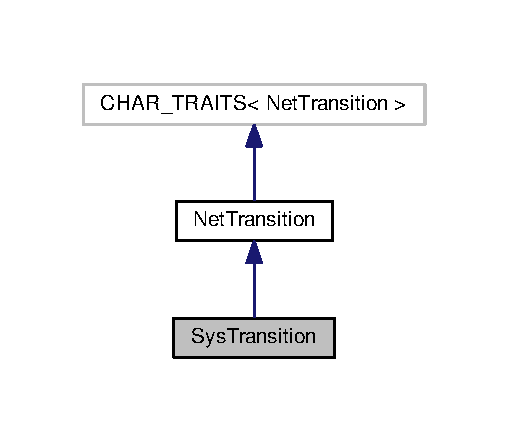
\includegraphics[width=244pt]{class_sys_transition__inherit__graph}
\end{center}
\end{figure}


Collaboration diagram for Sys\+Transition\+:
\nopagebreak
\begin{figure}[H]
\begin{center}
\leavevmode
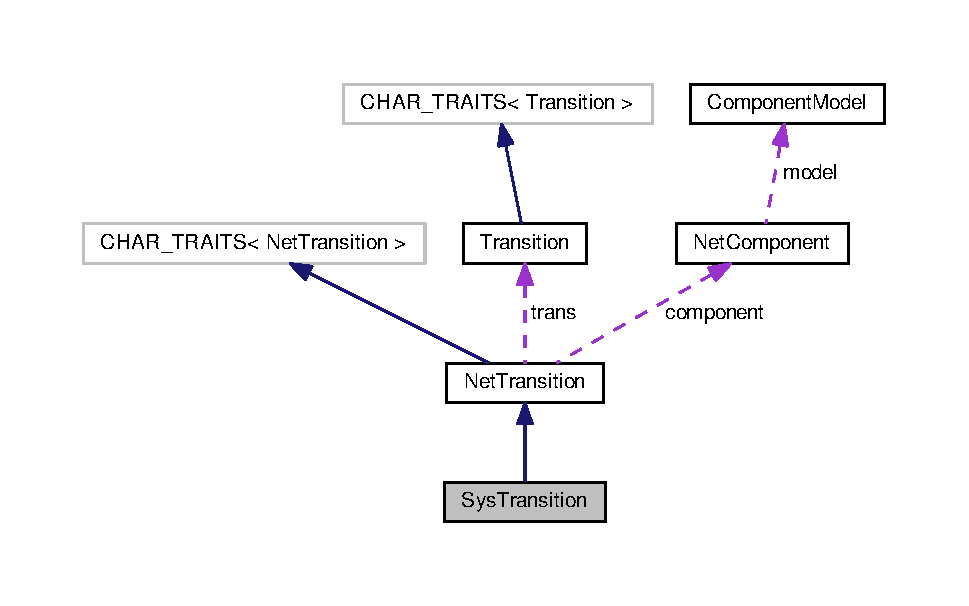
\includegraphics[width=350pt]{class_sys_transition__coll__graph}
\end{center}
\end{figure}
\subsection*{Public Types}
\begin{DoxyCompactItemize}
\item 
typedef \hyperlink{class_sys_transition}{Sys\+Transition} \hyperlink{class_sys_transition_aa17f0f716cf9f7f3a860bf4606aea72a}{char\+\_\+type}\hypertarget{class_sys_transition_aa17f0f716cf9f7f3a860bf4606aea72a}{}\label{class_sys_transition_aa17f0f716cf9f7f3a860bf4606aea72a}

\begin{DoxyCompactList}\small\item\em char\+\_\+type \end{DoxyCompactList}\item 
typedef long \hyperlink{class_sys_transition_aa038700854a41ddc7c6d807250b515eb}{int\+\_\+type}\hypertarget{class_sys_transition_aa038700854a41ddc7c6d807250b515eb}{}\label{class_sys_transition_aa038700854a41ddc7c6d807250b515eb}

\begin{DoxyCompactList}\small\item\em int\+\_\+type \end{DoxyCompactList}\end{DoxyCompactItemize}
\subsection*{Public Member Functions}
\begin{DoxyCompactItemize}
\item 
\hyperlink{class_sys_transition_a3918816e3e9b4e505f1b8db508832cfb}{Sys\+Transition} ()\hypertarget{class_sys_transition_a3918816e3e9b4e505f1b8db508832cfb}{}\label{class_sys_transition_a3918816e3e9b4e505f1b8db508832cfb}

\begin{DoxyCompactList}\small\item\em \hyperlink{class_sys_transition}{Sys\+Transition}. \end{DoxyCompactList}\item 
\hyperlink{class_sys_transition_aa79fd80b8a077838873db93662accc2c}{Sys\+Transition} (\hyperlink{class_transition}{Transition} $\ast$t, \hyperlink{class_net_component}{Net\+Component} $\ast$c, \hyperlink{class_system_node}{System\+Node} $\ast$n)
\begin{DoxyCompactList}\small\item\em \hyperlink{class_sys_transition}{Sys\+Transition}. \end{DoxyCompactList}\item 
\hyperlink{class_system_node}{System\+Node} $\ast$ \hyperlink{class_sys_transition_afc54d9b7708e2d80761e9fa99a6d1bfb}{get\+\_\+node} () const 
\begin{DoxyCompactList}\small\item\em get\+\_\+node \end{DoxyCompactList}\item 
pair$<$ string, string $>$ \hyperlink{class_sys_transition_a6ed437db199f6ccbd8578e1db305a221}{get\+\_\+t\+\_\+name\+\_\+c\+\_\+name} () const 
\begin{DoxyCompactList}\small\item\em get\+\_\+t\+\_\+name\+\_\+c\+\_\+name \end{DoxyCompactList}\item 
void \hyperlink{class_sys_transition_a6cd5c8bb1f39370c8c4552cea193caf0}{set\+\_\+input\+\_\+event} (std\+::string e, int index)
\begin{DoxyCompactList}\small\item\em set\+\_\+input\+\_\+event \end{DoxyCompactList}\item 
void \hyperlink{class_sys_transition_a6a04aa7872a8d891d085764bca41c9cd}{add\+\_\+output\+\_\+event} (std\+::string e, vector$<$ int $>$ indexes)
\begin{DoxyCompactList}\small\item\em add\+\_\+output\+\_\+event \end{DoxyCompactList}\item 
void \hyperlink{class_sys_transition_a1a467d06dfa861340820815247fa0bab}{set\+\_\+lazy\+\_\+input\+\_\+event} (std\+::string e, int index)
\begin{DoxyCompactList}\small\item\em set\+\_\+lazy\+\_\+input\+\_\+event \end{DoxyCompactList}\item 
void \hyperlink{class_sys_transition_ac97ba8c514e4925a7b86dacf31a69a7d}{add\+\_\+lazy\+\_\+output\+\_\+event} (std\+::string e, vector$<$ int $>$ indexes)
\begin{DoxyCompactList}\small\item\em add\+\_\+lazy\+\_\+output\+\_\+event \end{DoxyCompactList}\item 
bool \hyperlink{class_sys_transition_aa46d54c147f5a7c1aa1442d7612953f4}{is\+\_\+triggerable} (vector$<$ string $>$ \&E, bool lazy=false)
\begin{DoxyCompactList}\small\item\em is\+\_\+triggerable checks if current transition is triggerable (saturation policy W\+A\+IT) \end{DoxyCompactList}\item 
void \hyperlink{class_sys_transition_aca76296b036d975c4df4e22169b20028}{effects} (vector$<$ string $>$ \&E, bool lazy=false)
\begin{DoxyCompactList}\small\item\em effects computes new configuration of input terminals after transition execution \end{DoxyCompactList}\item 
bool \hyperlink{class_sys_transition_a91b3fe79173a73dbe6698c5b31f952e3}{operator$<$} (const \hyperlink{class_sys_transition}{Sys\+Transition} t) const 
\begin{DoxyCompactList}\small\item\em operator $<$ \end{DoxyCompactList}\item 
bool \hyperlink{class_sys_transition_a7f7fc86a8a9aa93bc2c46ce4b9bdbc7d}{operator==} (const \hyperlink{class_sys_transition}{Sys\+Transition} t) const 
\begin{DoxyCompactList}\small\item\em operator == \end{DoxyCompactList}\end{DoxyCompactItemize}
\subsection*{Static Public Member Functions}
\begin{DoxyCompactItemize}
\item 
static bool \hyperlink{class_sys_transition_a500b0625bdf4376bd9e8efe5ab95a3c6}{eq} (const \hyperlink{class_net_transition_a40ad367a5a816d31e7559037c76970f0}{char\+\_\+type} \&x, const \hyperlink{class_net_transition_a40ad367a5a816d31e7559037c76970f0}{char\+\_\+type} \&y)
\begin{DoxyCompactList}\small\item\em eq \end{DoxyCompactList}\item 
static bool \hyperlink{class_sys_transition_af4a28bd6c0b91618fb8e7f78c4a7e9dc}{lt} (const \hyperlink{class_net_transition_a40ad367a5a816d31e7559037c76970f0}{char\+\_\+type} \&x, const \hyperlink{class_net_transition_a40ad367a5a816d31e7559037c76970f0}{char\+\_\+type} \&y)
\begin{DoxyCompactList}\small\item\em lt \end{DoxyCompactList}\end{DoxyCompactItemize}
\subsection*{Static Public Attributes}
\begin{DoxyCompactItemize}
\item 
static const size\+\_\+t \hyperlink{class_sys_transition_a18c0e61e238edb4d01c9cefff242cf7b}{size}\hypertarget{class_sys_transition_a18c0e61e238edb4d01c9cefff242cf7b}{}\label{class_sys_transition_a18c0e61e238edb4d01c9cefff242cf7b}

\begin{DoxyCompactList}\small\item\em size \end{DoxyCompactList}\end{DoxyCompactItemize}
\subsection*{Friends}
\begin{DoxyCompactItemize}
\item 
class {\bfseries boost\+::serialization\+::access}\hypertarget{class_sys_transition_ac98d07dd8f7b70e16ccb9a01abf56b9c}{}\label{class_sys_transition_ac98d07dd8f7b70e16ccb9a01abf56b9c}

\end{DoxyCompactItemize}
\subsection*{Additional Inherited Members}


\subsection{Detailed Description}
The \hyperlink{class_sys_transition}{Sys\+Transition} class represents a transition in a specific problem node. 

\begin{DoxyDate}{Date}
Febbraio 2016 
\end{DoxyDate}
\begin{DoxyAuthor}{Author}
Giulio Quarenghi 
\end{DoxyAuthor}


\subsection{Constructor \& Destructor Documentation}
\index{Sys\+Transition@{Sys\+Transition}!Sys\+Transition@{Sys\+Transition}}
\index{Sys\+Transition@{Sys\+Transition}!Sys\+Transition@{Sys\+Transition}}
\subsubsection[{\texorpdfstring{Sys\+Transition(\+Transition $\ast$t, Net\+Component $\ast$c, System\+Node $\ast$n)}{SysTransition(Transition *t, NetComponent *c, SystemNode *n)}}]{\setlength{\rightskip}{0pt plus 5cm}Sys\+Transition\+::\+Sys\+Transition (
\begin{DoxyParamCaption}
\item[{{\bf Transition} $\ast$}]{t, }
\item[{{\bf Net\+Component} $\ast$}]{c, }
\item[{{\bf System\+Node} $\ast$}]{n}
\end{DoxyParamCaption}
)}\hypertarget{class_sys_transition_aa79fd80b8a077838873db93662accc2c}{}\label{class_sys_transition_aa79fd80b8a077838873db93662accc2c}


\hyperlink{class_sys_transition}{Sys\+Transition}. 


\begin{DoxyParams}{Parameters}
{\em t} & \\
\hline
{\em c} & \\
\hline
{\em n} & \\
\hline
\end{DoxyParams}


\subsection{Member Function Documentation}
\index{Sys\+Transition@{Sys\+Transition}!add\+\_\+lazy\+\_\+output\+\_\+event@{add\+\_\+lazy\+\_\+output\+\_\+event}}
\index{add\+\_\+lazy\+\_\+output\+\_\+event@{add\+\_\+lazy\+\_\+output\+\_\+event}!Sys\+Transition@{Sys\+Transition}}
\subsubsection[{\texorpdfstring{add\+\_\+lazy\+\_\+output\+\_\+event(std\+::string e, vector$<$ int $>$ indexes)}{add_lazy_output_event(std::string e, vector< int > indexes)}}]{\setlength{\rightskip}{0pt plus 5cm}void Sys\+Transition\+::add\+\_\+lazy\+\_\+output\+\_\+event (
\begin{DoxyParamCaption}
\item[{std\+::string}]{e, }
\item[{vector$<$ int $>$}]{indexes}
\end{DoxyParamCaption}
)}\hypertarget{class_sys_transition_ac97ba8c514e4925a7b86dacf31a69a7d}{}\label{class_sys_transition_ac97ba8c514e4925a7b86dacf31a69a7d}


add\+\_\+lazy\+\_\+output\+\_\+event 


\begin{DoxyParams}{Parameters}
{\em e} & \\
\hline
{\em indexes} & \\
\hline
\end{DoxyParams}
\index{Sys\+Transition@{Sys\+Transition}!add\+\_\+output\+\_\+event@{add\+\_\+output\+\_\+event}}
\index{add\+\_\+output\+\_\+event@{add\+\_\+output\+\_\+event}!Sys\+Transition@{Sys\+Transition}}
\subsubsection[{\texorpdfstring{add\+\_\+output\+\_\+event(std\+::string e, vector$<$ int $>$ indexes)}{add_output_event(std::string e, vector< int > indexes)}}]{\setlength{\rightskip}{0pt plus 5cm}void Sys\+Transition\+::add\+\_\+output\+\_\+event (
\begin{DoxyParamCaption}
\item[{std\+::string}]{e, }
\item[{vector$<$ int $>$}]{indexes}
\end{DoxyParamCaption}
)}\hypertarget{class_sys_transition_a6a04aa7872a8d891d085764bca41c9cd}{}\label{class_sys_transition_a6a04aa7872a8d891d085764bca41c9cd}


add\+\_\+output\+\_\+event 


\begin{DoxyParams}{Parameters}
{\em e} & \\
\hline
{\em indexes} & \\
\hline
\end{DoxyParams}
\index{Sys\+Transition@{Sys\+Transition}!effects@{effects}}
\index{effects@{effects}!Sys\+Transition@{Sys\+Transition}}
\subsubsection[{\texorpdfstring{effects(vector$<$ string $>$ \&\+E, bool lazy=false)}{effects(vector< string > &E, bool lazy=false)}}]{\setlength{\rightskip}{0pt plus 5cm}void Sys\+Transition\+::effects (
\begin{DoxyParamCaption}
\item[{vector$<$ string $>$ \&}]{E, }
\item[{bool}]{lazy = {\ttfamily false}}
\end{DoxyParamCaption}
)}\hypertarget{class_sys_transition_aca76296b036d975c4df4e22169b20028}{}\label{class_sys_transition_aca76296b036d975c4df4e22169b20028}


effects computes new configuration of input terminals after transition execution 


\begin{DoxyParams}{Parameters}
{\em E} & input terminals values \\
\hline
{\em lazy} & true if diagnosis is in lazy mode, false otherwise \\
\hline
\end{DoxyParams}
\index{Sys\+Transition@{Sys\+Transition}!eq@{eq}}
\index{eq@{eq}!Sys\+Transition@{Sys\+Transition}}
\subsubsection[{\texorpdfstring{eq(const char\+\_\+type \&x, const char\+\_\+type \&y)}{eq(const char_type &x, const char_type &y)}}]{\setlength{\rightskip}{0pt plus 5cm}static bool Sys\+Transition\+::eq (
\begin{DoxyParamCaption}
\item[{const {\bf char\+\_\+type} \&}]{x, }
\item[{const {\bf char\+\_\+type} \&}]{y}
\end{DoxyParamCaption}
)\hspace{0.3cm}{\ttfamily [inline]}, {\ttfamily [static]}}\hypertarget{class_sys_transition_a500b0625bdf4376bd9e8efe5ab95a3c6}{}\label{class_sys_transition_a500b0625bdf4376bd9e8efe5ab95a3c6}


eq 


\begin{DoxyParams}{Parameters}
{\em x} & \\
\hline
{\em y} & \\
\hline
\end{DoxyParams}
\begin{DoxyReturn}{Returns}

\end{DoxyReturn}
\index{Sys\+Transition@{Sys\+Transition}!get\+\_\+node@{get\+\_\+node}}
\index{get\+\_\+node@{get\+\_\+node}!Sys\+Transition@{Sys\+Transition}}
\subsubsection[{\texorpdfstring{get\+\_\+node() const }{get_node() const }}]{\setlength{\rightskip}{0pt plus 5cm}{\bf System\+Node} $\ast$ Sys\+Transition\+::get\+\_\+node (
\begin{DoxyParamCaption}
{}
\end{DoxyParamCaption}
) const}\hypertarget{class_sys_transition_afc54d9b7708e2d80761e9fa99a6d1bfb}{}\label{class_sys_transition_afc54d9b7708e2d80761e9fa99a6d1bfb}


get\+\_\+node 

\begin{DoxyReturn}{Returns}

\end{DoxyReturn}
\index{Sys\+Transition@{Sys\+Transition}!get\+\_\+t\+\_\+name\+\_\+c\+\_\+name@{get\+\_\+t\+\_\+name\+\_\+c\+\_\+name}}
\index{get\+\_\+t\+\_\+name\+\_\+c\+\_\+name@{get\+\_\+t\+\_\+name\+\_\+c\+\_\+name}!Sys\+Transition@{Sys\+Transition}}
\subsubsection[{\texorpdfstring{get\+\_\+t\+\_\+name\+\_\+c\+\_\+name() const }{get_t_name_c_name() const }}]{\setlength{\rightskip}{0pt plus 5cm}pair$<$ string, string $>$ Sys\+Transition\+::get\+\_\+t\+\_\+name\+\_\+c\+\_\+name (
\begin{DoxyParamCaption}
{}
\end{DoxyParamCaption}
) const}\hypertarget{class_sys_transition_a6ed437db199f6ccbd8578e1db305a221}{}\label{class_sys_transition_a6ed437db199f6ccbd8578e1db305a221}


get\+\_\+t\+\_\+name\+\_\+c\+\_\+name 

\begin{DoxyReturn}{Returns}

\end{DoxyReturn}
\index{Sys\+Transition@{Sys\+Transition}!is\+\_\+triggerable@{is\+\_\+triggerable}}
\index{is\+\_\+triggerable@{is\+\_\+triggerable}!Sys\+Transition@{Sys\+Transition}}
\subsubsection[{\texorpdfstring{is\+\_\+triggerable(vector$<$ string $>$ \&\+E, bool lazy=false)}{is_triggerable(vector< string > &E, bool lazy=false)}}]{\setlength{\rightskip}{0pt plus 5cm}bool Sys\+Transition\+::is\+\_\+triggerable (
\begin{DoxyParamCaption}
\item[{vector$<$ string $>$ \&}]{E, }
\item[{bool}]{lazy = {\ttfamily false}}
\end{DoxyParamCaption}
)}\hypertarget{class_sys_transition_aa46d54c147f5a7c1aa1442d7612953f4}{}\label{class_sys_transition_aa46d54c147f5a7c1aa1442d7612953f4}


is\+\_\+triggerable checks if current transition is triggerable (saturation policy W\+A\+IT) 


\begin{DoxyParams}{Parameters}
{\em E} & current configuration of input terminals content \\
\hline
{\em lazy} & true if diagnosis is in lazy mode, false otherwise \\
\hline
\end{DoxyParams}
\begin{DoxyReturn}{Returns}
true of transition is triggerable, false otherwise 
\end{DoxyReturn}
\index{Sys\+Transition@{Sys\+Transition}!lt@{lt}}
\index{lt@{lt}!Sys\+Transition@{Sys\+Transition}}
\subsubsection[{\texorpdfstring{lt(const char\+\_\+type \&x, const char\+\_\+type \&y)}{lt(const char_type &x, const char_type &y)}}]{\setlength{\rightskip}{0pt plus 5cm}static bool Sys\+Transition\+::lt (
\begin{DoxyParamCaption}
\item[{const {\bf char\+\_\+type} \&}]{x, }
\item[{const {\bf char\+\_\+type} \&}]{y}
\end{DoxyParamCaption}
)\hspace{0.3cm}{\ttfamily [inline]}, {\ttfamily [static]}}\hypertarget{class_sys_transition_af4a28bd6c0b91618fb8e7f78c4a7e9dc}{}\label{class_sys_transition_af4a28bd6c0b91618fb8e7f78c4a7e9dc}


lt 


\begin{DoxyParams}{Parameters}
{\em x} & \\
\hline
{\em y} & \\
\hline
\end{DoxyParams}
\begin{DoxyReturn}{Returns}

\end{DoxyReturn}
\index{Sys\+Transition@{Sys\+Transition}!operator$<$@{operator$<$}}
\index{operator$<$@{operator$<$}!Sys\+Transition@{Sys\+Transition}}
\subsubsection[{\texorpdfstring{operator$<$(const Sys\+Transition t) const }{operator<(const SysTransition t) const }}]{\setlength{\rightskip}{0pt plus 5cm}bool Sys\+Transition\+::operator$<$ (
\begin{DoxyParamCaption}
\item[{const {\bf Sys\+Transition}}]{t}
\end{DoxyParamCaption}
) const\hspace{0.3cm}{\ttfamily [inline]}}\hypertarget{class_sys_transition_a91b3fe79173a73dbe6698c5b31f952e3}{}\label{class_sys_transition_a91b3fe79173a73dbe6698c5b31f952e3}


operator $<$ 


\begin{DoxyParams}{Parameters}
{\em t} & \\
\hline
\end{DoxyParams}
\begin{DoxyReturn}{Returns}

\end{DoxyReturn}
\index{Sys\+Transition@{Sys\+Transition}!operator==@{operator==}}
\index{operator==@{operator==}!Sys\+Transition@{Sys\+Transition}}
\subsubsection[{\texorpdfstring{operator==(const Sys\+Transition t) const }{operator==(const SysTransition t) const }}]{\setlength{\rightskip}{0pt plus 5cm}bool Sys\+Transition\+::operator== (
\begin{DoxyParamCaption}
\item[{const {\bf Sys\+Transition}}]{t}
\end{DoxyParamCaption}
) const\hspace{0.3cm}{\ttfamily [inline]}}\hypertarget{class_sys_transition_a7f7fc86a8a9aa93bc2c46ce4b9bdbc7d}{}\label{class_sys_transition_a7f7fc86a8a9aa93bc2c46ce4b9bdbc7d}


operator == 


\begin{DoxyParams}{Parameters}
{\em t} & \\
\hline
\end{DoxyParams}
\begin{DoxyReturn}{Returns}

\end{DoxyReturn}
\index{Sys\+Transition@{Sys\+Transition}!set\+\_\+input\+\_\+event@{set\+\_\+input\+\_\+event}}
\index{set\+\_\+input\+\_\+event@{set\+\_\+input\+\_\+event}!Sys\+Transition@{Sys\+Transition}}
\subsubsection[{\texorpdfstring{set\+\_\+input\+\_\+event(std\+::string e, int index)}{set_input_event(std::string e, int index)}}]{\setlength{\rightskip}{0pt plus 5cm}void Sys\+Transition\+::set\+\_\+input\+\_\+event (
\begin{DoxyParamCaption}
\item[{std\+::string}]{e, }
\item[{int}]{index}
\end{DoxyParamCaption}
)}\hypertarget{class_sys_transition_a6cd5c8bb1f39370c8c4552cea193caf0}{}\label{class_sys_transition_a6cd5c8bb1f39370c8c4552cea193caf0}


set\+\_\+input\+\_\+event 


\begin{DoxyParams}{Parameters}
{\em e} & \\
\hline
{\em index} & \\
\hline
\end{DoxyParams}
\index{Sys\+Transition@{Sys\+Transition}!set\+\_\+lazy\+\_\+input\+\_\+event@{set\+\_\+lazy\+\_\+input\+\_\+event}}
\index{set\+\_\+lazy\+\_\+input\+\_\+event@{set\+\_\+lazy\+\_\+input\+\_\+event}!Sys\+Transition@{Sys\+Transition}}
\subsubsection[{\texorpdfstring{set\+\_\+lazy\+\_\+input\+\_\+event(std\+::string e, int index)}{set_lazy_input_event(std::string e, int index)}}]{\setlength{\rightskip}{0pt plus 5cm}void Sys\+Transition\+::set\+\_\+lazy\+\_\+input\+\_\+event (
\begin{DoxyParamCaption}
\item[{std\+::string}]{e, }
\item[{int}]{index}
\end{DoxyParamCaption}
)}\hypertarget{class_sys_transition_a1a467d06dfa861340820815247fa0bab}{}\label{class_sys_transition_a1a467d06dfa861340820815247fa0bab}


set\+\_\+lazy\+\_\+input\+\_\+event 


\begin{DoxyParams}{Parameters}
{\em e} & \\
\hline
{\em index} & \\
\hline
\end{DoxyParams}


The documentation for this class was generated from the following files\+:\begin{DoxyCompactItemize}
\item 
systransition.\+h\item 
systransition.\+cpp\end{DoxyCompactItemize}

\hypertarget{class_terminal}{}\section{Terminal Class Reference}
\label{class_terminal}\index{Terminal@{Terminal}}


The \hyperlink{class_terminal}{Terminal} class represents concrete terminals of components and problem nodes.  




{\ttfamily \#include $<$terminal.\+h$>$}

\subsection*{Public Member Functions}
\begin{DoxyCompactItemize}
\item 
\hyperlink{class_terminal_aa448509b5aa1ece53c3d86385655be0e}{Terminal} ()\hypertarget{class_terminal_aa448509b5aa1ece53c3d86385655be0e}{}\label{class_terminal_aa448509b5aa1ece53c3d86385655be0e}

\begin{DoxyCompactList}\small\item\em \hyperlink{class_terminal}{Terminal}. \end{DoxyCompactList}\item 
\hyperlink{class_terminal_a528fbc18108f9396d969775453851efe}{Terminal} (std\+::string n)
\begin{DoxyCompactList}\small\item\em \hyperlink{class_terminal}{Terminal}. \end{DoxyCompactList}\item 
std\+::string \hyperlink{class_terminal_a79757bf237bac0a7d988ca61938f2bec}{get\+\_\+name} () const 
\begin{DoxyCompactList}\small\item\em get\+\_\+name \end{DoxyCompactList}\item 
std\+::string \hyperlink{class_terminal_a74dc0c5c76ec9a03f2efed4dae74b7a5}{get\+\_\+value} () const 
\begin{DoxyCompactList}\small\item\em get\+\_\+value \end{DoxyCompactList}\item 
std\+::vector$<$ \hyperlink{class_terminal}{Terminal} $\ast$ $>$ \hyperlink{class_terminal_a9ca76f85961beb83450055da4e559b48}{get\+\_\+linked\+\_\+terminals} () const 
\begin{DoxyCompactList}\small\item\em get\+\_\+linked\+\_\+terminals \end{DoxyCompactList}\item 
void \hyperlink{class_terminal_a2772ca04d4b5e6f468eaa8fca866c171}{set\+\_\+value} (std\+::string v)
\begin{DoxyCompactList}\small\item\em set\+\_\+value \end{DoxyCompactList}\item 
void \hyperlink{class_terminal_a46b1e64649f14e8443403f9ef8aa6342}{add\+\_\+linked\+\_\+terminal} (\hyperlink{class_terminal}{Terminal} $\ast$t)
\begin{DoxyCompactList}\small\item\em add\+\_\+linked\+\_\+terminal \end{DoxyCompactList}\end{DoxyCompactItemize}
\subsection*{Friends}
\begin{DoxyCompactItemize}
\item 
class {\bfseries boost\+::serialization\+::access}\hypertarget{class_terminal_ac98d07dd8f7b70e16ccb9a01abf56b9c}{}\label{class_terminal_ac98d07dd8f7b70e16ccb9a01abf56b9c}

\end{DoxyCompactItemize}


\subsection{Detailed Description}
The \hyperlink{class_terminal}{Terminal} class represents concrete terminals of components and problem nodes. 

\begin{DoxyDate}{Date}
Febbraio 2016 
\end{DoxyDate}
\begin{DoxyAuthor}{Author}
Giulio Quarenghi 
\end{DoxyAuthor}


\subsection{Constructor \& Destructor Documentation}
\index{Terminal@{Terminal}!Terminal@{Terminal}}
\index{Terminal@{Terminal}!Terminal@{Terminal}}
\subsubsection[{\texorpdfstring{Terminal(std\+::string n)}{Terminal(std::string n)}}]{\setlength{\rightskip}{0pt plus 5cm}Terminal\+::\+Terminal (
\begin{DoxyParamCaption}
\item[{std\+::string}]{n}
\end{DoxyParamCaption}
)}\hypertarget{class_terminal_a528fbc18108f9396d969775453851efe}{}\label{class_terminal_a528fbc18108f9396d969775453851efe}


\hyperlink{class_terminal}{Terminal}. 


\begin{DoxyParams}{Parameters}
{\em n} & \\
\hline
\end{DoxyParams}


\subsection{Member Function Documentation}
\index{Terminal@{Terminal}!add\+\_\+linked\+\_\+terminal@{add\+\_\+linked\+\_\+terminal}}
\index{add\+\_\+linked\+\_\+terminal@{add\+\_\+linked\+\_\+terminal}!Terminal@{Terminal}}
\subsubsection[{\texorpdfstring{add\+\_\+linked\+\_\+terminal(\+Terminal $\ast$t)}{add_linked_terminal(Terminal *t)}}]{\setlength{\rightskip}{0pt plus 5cm}void Terminal\+::add\+\_\+linked\+\_\+terminal (
\begin{DoxyParamCaption}
\item[{{\bf Terminal} $\ast$}]{t}
\end{DoxyParamCaption}
)}\hypertarget{class_terminal_a46b1e64649f14e8443403f9ef8aa6342}{}\label{class_terminal_a46b1e64649f14e8443403f9ef8aa6342}


add\+\_\+linked\+\_\+terminal 


\begin{DoxyParams}{Parameters}
{\em t} & \\
\hline
\end{DoxyParams}
\index{Terminal@{Terminal}!get\+\_\+linked\+\_\+terminals@{get\+\_\+linked\+\_\+terminals}}
\index{get\+\_\+linked\+\_\+terminals@{get\+\_\+linked\+\_\+terminals}!Terminal@{Terminal}}
\subsubsection[{\texorpdfstring{get\+\_\+linked\+\_\+terminals() const }{get_linked_terminals() const }}]{\setlength{\rightskip}{0pt plus 5cm}std\+::vector$<$ {\bf Terminal} $\ast$ $>$ Terminal\+::get\+\_\+linked\+\_\+terminals (
\begin{DoxyParamCaption}
{}
\end{DoxyParamCaption}
) const}\hypertarget{class_terminal_a9ca76f85961beb83450055da4e559b48}{}\label{class_terminal_a9ca76f85961beb83450055da4e559b48}


get\+\_\+linked\+\_\+terminals 

\begin{DoxyReturn}{Returns}

\end{DoxyReturn}
\index{Terminal@{Terminal}!get\+\_\+name@{get\+\_\+name}}
\index{get\+\_\+name@{get\+\_\+name}!Terminal@{Terminal}}
\subsubsection[{\texorpdfstring{get\+\_\+name() const }{get_name() const }}]{\setlength{\rightskip}{0pt plus 5cm}std\+::string Terminal\+::get\+\_\+name (
\begin{DoxyParamCaption}
{}
\end{DoxyParamCaption}
) const}\hypertarget{class_terminal_a79757bf237bac0a7d988ca61938f2bec}{}\label{class_terminal_a79757bf237bac0a7d988ca61938f2bec}


get\+\_\+name 

\begin{DoxyReturn}{Returns}

\end{DoxyReturn}
\index{Terminal@{Terminal}!get\+\_\+value@{get\+\_\+value}}
\index{get\+\_\+value@{get\+\_\+value}!Terminal@{Terminal}}
\subsubsection[{\texorpdfstring{get\+\_\+value() const }{get_value() const }}]{\setlength{\rightskip}{0pt plus 5cm}std\+::string Terminal\+::get\+\_\+value (
\begin{DoxyParamCaption}
{}
\end{DoxyParamCaption}
) const}\hypertarget{class_terminal_a74dc0c5c76ec9a03f2efed4dae74b7a5}{}\label{class_terminal_a74dc0c5c76ec9a03f2efed4dae74b7a5}


get\+\_\+value 

\begin{DoxyReturn}{Returns}

\end{DoxyReturn}
\index{Terminal@{Terminal}!set\+\_\+value@{set\+\_\+value}}
\index{set\+\_\+value@{set\+\_\+value}!Terminal@{Terminal}}
\subsubsection[{\texorpdfstring{set\+\_\+value(std\+::string v)}{set_value(std::string v)}}]{\setlength{\rightskip}{0pt plus 5cm}void Terminal\+::set\+\_\+value (
\begin{DoxyParamCaption}
\item[{std\+::string}]{v}
\end{DoxyParamCaption}
)}\hypertarget{class_terminal_a2772ca04d4b5e6f468eaa8fca866c171}{}\label{class_terminal_a2772ca04d4b5e6f468eaa8fca866c171}


set\+\_\+value 


\begin{DoxyParams}{Parameters}
{\em v} & \\
\hline
\end{DoxyParams}


The documentation for this class was generated from the following files\+:\begin{DoxyCompactItemize}
\item 
terminal.\+h\item 
terminal.\+cpp\end{DoxyCompactItemize}

\hypertarget{class_transition}{}\section{Transition Class Reference}
\label{class_transition}\index{Transition@{Transition}}


The \hyperlink{class_transition}{Transition} class.  




{\ttfamily \#include $<$transition.\+h$>$}



Inheritance diagram for Transition\+:\nopagebreak
\begin{figure}[H]
\begin{center}
\leavevmode
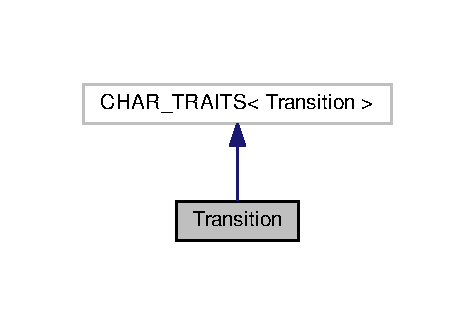
\includegraphics[width=228pt]{class_transition__inherit__graph}
\end{center}
\end{figure}


Collaboration diagram for Transition\+:\nopagebreak
\begin{figure}[H]
\begin{center}
\leavevmode
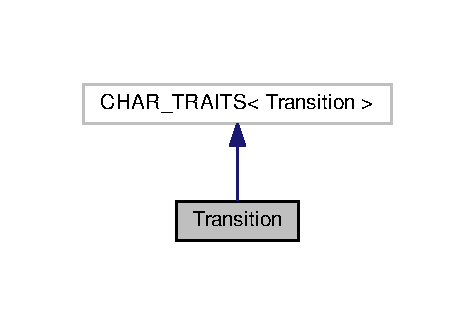
\includegraphics[width=228pt]{class_transition__coll__graph}
\end{center}
\end{figure}
\subsection*{Public Types}
\begin{DoxyCompactItemize}
\item 
typedef \hyperlink{class_transition}{Transition} \hyperlink{class_transition_a701b8dd85eadbda28008778631ed9c08}{char\+\_\+type}\hypertarget{class_transition_a701b8dd85eadbda28008778631ed9c08}{}\label{class_transition_a701b8dd85eadbda28008778631ed9c08}

\begin{DoxyCompactList}\small\item\em char\+\_\+type \end{DoxyCompactList}\item 
typedef long \hyperlink{class_transition_a2a84af67283a25a2fc2ddd276092adbb}{int\+\_\+type}\hypertarget{class_transition_a2a84af67283a25a2fc2ddd276092adbb}{}\label{class_transition_a2a84af67283a25a2fc2ddd276092adbb}

\begin{DoxyCompactList}\small\item\em int\+\_\+type \end{DoxyCompactList}\end{DoxyCompactItemize}
\subsection*{Public Member Functions}
\begin{DoxyCompactItemize}
\item 
\hyperlink{class_transition_a73b44b2338b11807f77b620a3e810f92}{Transition} ()\hypertarget{class_transition_a73b44b2338b11807f77b620a3e810f92}{}\label{class_transition_a73b44b2338b11807f77b620a3e810f92}

\begin{DoxyCompactList}\small\item\em \hyperlink{class_transition}{Transition}. \end{DoxyCompactList}\item 
\hyperlink{class_transition_a2455a9d73049ae0fe4edba67be1cb62d}{Transition} (std\+::string n)
\begin{DoxyCompactList}\small\item\em \hyperlink{class_transition}{Transition}. \end{DoxyCompactList}\item 
std\+::string \hyperlink{class_transition_afb2e105b100da66587695033bf45ed0e}{get\+\_\+name} () const 
\begin{DoxyCompactList}\small\item\em get\+\_\+name \end{DoxyCompactList}\item 
std\+::pair$<$ std\+::string, std\+::string $>$ \hyperlink{class_transition_aa9a28517d94919fccfb147c8a0ad4dc0}{get\+\_\+input\+\_\+event} () const 
\begin{DoxyCompactList}\small\item\em get\+\_\+input\+\_\+event \end{DoxyCompactList}\item 
std\+::pair$<$ std\+::string, std\+::string $>$ \hyperlink{class_transition_a173debd0cd54c3a87ecdfba9ab761f80}{get\+\_\+s1\+\_\+s2} () const 
\begin{DoxyCompactList}\small\item\em get\+\_\+s1\+\_\+s2 \end{DoxyCompactList}\item 
std\+::vector$<$ std\+::pair$<$ std\+::string, std\+::string $>$ $>$ \hyperlink{class_transition_ade549af354654b844af6d54693f4af6a}{get\+\_\+out\+\_\+events} () const 
\begin{DoxyCompactList}\small\item\em get\+\_\+out\+\_\+events \end{DoxyCompactList}\item 
void \hyperlink{class_transition_a4b220aa7b2001942e23ab15075f1aa31}{set\+\_\+input\+\_\+event} (std\+::string e, std\+::string t)
\begin{DoxyCompactList}\small\item\em set\+\_\+input\+\_\+event \end{DoxyCompactList}\item 
void \hyperlink{class_transition_ae5aafaf781f86a2cdd5e72fb19d97f5f}{set\+\_\+s1\+\_\+s2} (std\+::string s1, std\+::string s2)
\begin{DoxyCompactList}\small\item\em set\+\_\+s1\+\_\+s2 \end{DoxyCompactList}\item 
void \hyperlink{class_transition_a2520c6cc0f7e6607341f6d8f20e45d28}{add\+\_\+out\+\_\+event} (std\+::string e, std\+::string t)
\begin{DoxyCompactList}\small\item\em add\+\_\+out\+\_\+event \end{DoxyCompactList}\item 
void \hyperlink{class_transition_acf51ad82dfa53f630e34f8c61cc3fbfb}{set\+\_\+out\+\_\+events} (std\+::vector$<$ std\+::pair$<$ std\+::string, std\+::string $>$ $>$ evs)
\begin{DoxyCompactList}\small\item\em set\+\_\+out\+\_\+events \end{DoxyCompactList}\item 
bool \hyperlink{class_transition_abb05ffb0eafbc0b97a478e7a3a266609}{operator$<$} (const \hyperlink{class_transition}{Transition} t) const 
\begin{DoxyCompactList}\small\item\em operator $<$ \end{DoxyCompactList}\item 
bool \hyperlink{class_transition_af76ce33a5b0b44fbd87c17e872d32d8c}{operator==} (const \hyperlink{class_transition}{Transition} t) const 
\begin{DoxyCompactList}\small\item\em operator == \end{DoxyCompactList}\end{DoxyCompactItemize}
\subsection*{Static Public Member Functions}
\begin{DoxyCompactItemize}
\item 
static bool \hyperlink{class_transition_aff29b326d916908afcbb377178d34e43}{eq} (const \hyperlink{class_transition_a701b8dd85eadbda28008778631ed9c08}{char\+\_\+type} \&x, const \hyperlink{class_transition_a701b8dd85eadbda28008778631ed9c08}{char\+\_\+type} \&y)
\begin{DoxyCompactList}\small\item\em eq \end{DoxyCompactList}\item 
static bool \hyperlink{class_transition_ad1b2ae9ff8cde5bb8888fb6002cfa671}{lt} (const \hyperlink{class_transition_a701b8dd85eadbda28008778631ed9c08}{char\+\_\+type} \&x, const \hyperlink{class_transition_a701b8dd85eadbda28008778631ed9c08}{char\+\_\+type} \&y)
\begin{DoxyCompactList}\small\item\em lt \end{DoxyCompactList}\end{DoxyCompactItemize}
\subsection*{Static Public Attributes}
\begin{DoxyCompactItemize}
\item 
static const size\+\_\+t \hyperlink{class_transition_a579785c1d2d34e7dab5d34495041e004}{size}\hypertarget{class_transition_a579785c1d2d34e7dab5d34495041e004}{}\label{class_transition_a579785c1d2d34e7dab5d34495041e004}

\begin{DoxyCompactList}\small\item\em size \end{DoxyCompactList}\end{DoxyCompactItemize}
\subsection*{Friends}
\begin{DoxyCompactItemize}
\item 
class {\bfseries boost\+::serialization\+::access}\hypertarget{class_transition_ac98d07dd8f7b70e16ccb9a01abf56b9c}{}\label{class_transition_ac98d07dd8f7b70e16ccb9a01abf56b9c}

\end{DoxyCompactItemize}


\subsection{Detailed Description}
The \hyperlink{class_transition}{Transition} class. 

\begin{DoxyDate}{Date}
Febbraio 2016 
\end{DoxyDate}
\begin{DoxyAuthor}{Author}
Giulio Quarenghi 
\end{DoxyAuthor}


\subsection{Constructor \& Destructor Documentation}
\index{Transition@{Transition}!Transition@{Transition}}
\index{Transition@{Transition}!Transition@{Transition}}
\subsubsection[{\texorpdfstring{Transition(std\+::string n)}{Transition(std::string n)}}]{\setlength{\rightskip}{0pt plus 5cm}Transition\+::\+Transition (
\begin{DoxyParamCaption}
\item[{std\+::string}]{n}
\end{DoxyParamCaption}
)\hspace{0.3cm}{\ttfamily [inline]}}\hypertarget{class_transition_a2455a9d73049ae0fe4edba67be1cb62d}{}\label{class_transition_a2455a9d73049ae0fe4edba67be1cb62d}


\hyperlink{class_transition}{Transition}. 


\begin{DoxyParams}{Parameters}
{\em n} & \\
\hline
\end{DoxyParams}


\subsection{Member Function Documentation}
\index{Transition@{Transition}!add\+\_\+out\+\_\+event@{add\+\_\+out\+\_\+event}}
\index{add\+\_\+out\+\_\+event@{add\+\_\+out\+\_\+event}!Transition@{Transition}}
\subsubsection[{\texorpdfstring{add\+\_\+out\+\_\+event(std\+::string e, std\+::string t)}{add_out_event(std::string e, std::string t)}}]{\setlength{\rightskip}{0pt plus 5cm}void Transition\+::add\+\_\+out\+\_\+event (
\begin{DoxyParamCaption}
\item[{std\+::string}]{e, }
\item[{std\+::string}]{t}
\end{DoxyParamCaption}
)}\hypertarget{class_transition_a2520c6cc0f7e6607341f6d8f20e45d28}{}\label{class_transition_a2520c6cc0f7e6607341f6d8f20e45d28}


add\+\_\+out\+\_\+event 


\begin{DoxyParams}{Parameters}
{\em e} & \\
\hline
{\em t} & \\
\hline
\end{DoxyParams}
\index{Transition@{Transition}!eq@{eq}}
\index{eq@{eq}!Transition@{Transition}}
\subsubsection[{\texorpdfstring{eq(const char\+\_\+type \&x, const char\+\_\+type \&y)}{eq(const char_type &x, const char_type &y)}}]{\setlength{\rightskip}{0pt plus 5cm}static bool Transition\+::eq (
\begin{DoxyParamCaption}
\item[{const {\bf char\+\_\+type} \&}]{x, }
\item[{const {\bf char\+\_\+type} \&}]{y}
\end{DoxyParamCaption}
)\hspace{0.3cm}{\ttfamily [inline]}, {\ttfamily [static]}}\hypertarget{class_transition_aff29b326d916908afcbb377178d34e43}{}\label{class_transition_aff29b326d916908afcbb377178d34e43}


eq 


\begin{DoxyParams}{Parameters}
{\em x} & \\
\hline
{\em y} & \\
\hline
\end{DoxyParams}
\begin{DoxyReturn}{Returns}

\end{DoxyReturn}
\index{Transition@{Transition}!get\+\_\+input\+\_\+event@{get\+\_\+input\+\_\+event}}
\index{get\+\_\+input\+\_\+event@{get\+\_\+input\+\_\+event}!Transition@{Transition}}
\subsubsection[{\texorpdfstring{get\+\_\+input\+\_\+event() const }{get_input_event() const }}]{\setlength{\rightskip}{0pt plus 5cm}std\+::pair$<$ std\+::string, std\+::string $>$ Transition\+::get\+\_\+input\+\_\+event (
\begin{DoxyParamCaption}
{}
\end{DoxyParamCaption}
) const}\hypertarget{class_transition_aa9a28517d94919fccfb147c8a0ad4dc0}{}\label{class_transition_aa9a28517d94919fccfb147c8a0ad4dc0}


get\+\_\+input\+\_\+event 

\begin{DoxyReturn}{Returns}

\end{DoxyReturn}
\index{Transition@{Transition}!get\+\_\+name@{get\+\_\+name}}
\index{get\+\_\+name@{get\+\_\+name}!Transition@{Transition}}
\subsubsection[{\texorpdfstring{get\+\_\+name() const }{get_name() const }}]{\setlength{\rightskip}{0pt plus 5cm}std\+::string Transition\+::get\+\_\+name (
\begin{DoxyParamCaption}
{}
\end{DoxyParamCaption}
) const}\hypertarget{class_transition_afb2e105b100da66587695033bf45ed0e}{}\label{class_transition_afb2e105b100da66587695033bf45ed0e}


get\+\_\+name 

\begin{DoxyReturn}{Returns}

\end{DoxyReturn}
\index{Transition@{Transition}!get\+\_\+out\+\_\+events@{get\+\_\+out\+\_\+events}}
\index{get\+\_\+out\+\_\+events@{get\+\_\+out\+\_\+events}!Transition@{Transition}}
\subsubsection[{\texorpdfstring{get\+\_\+out\+\_\+events() const }{get_out_events() const }}]{\setlength{\rightskip}{0pt plus 5cm}std\+::vector$<$ std\+::pair$<$ std\+::string, std\+::string $>$ $>$ Transition\+::get\+\_\+out\+\_\+events (
\begin{DoxyParamCaption}
{}
\end{DoxyParamCaption}
) const}\hypertarget{class_transition_ade549af354654b844af6d54693f4af6a}{}\label{class_transition_ade549af354654b844af6d54693f4af6a}


get\+\_\+out\+\_\+events 

\begin{DoxyReturn}{Returns}

\end{DoxyReturn}
\index{Transition@{Transition}!get\+\_\+s1\+\_\+s2@{get\+\_\+s1\+\_\+s2}}
\index{get\+\_\+s1\+\_\+s2@{get\+\_\+s1\+\_\+s2}!Transition@{Transition}}
\subsubsection[{\texorpdfstring{get\+\_\+s1\+\_\+s2() const }{get_s1_s2() const }}]{\setlength{\rightskip}{0pt plus 5cm}std\+::pair$<$ std\+::string, std\+::string $>$ Transition\+::get\+\_\+s1\+\_\+s2 (
\begin{DoxyParamCaption}
{}
\end{DoxyParamCaption}
) const}\hypertarget{class_transition_a173debd0cd54c3a87ecdfba9ab761f80}{}\label{class_transition_a173debd0cd54c3a87ecdfba9ab761f80}


get\+\_\+s1\+\_\+s2 

\begin{DoxyReturn}{Returns}

\end{DoxyReturn}
\index{Transition@{Transition}!lt@{lt}}
\index{lt@{lt}!Transition@{Transition}}
\subsubsection[{\texorpdfstring{lt(const char\+\_\+type \&x, const char\+\_\+type \&y)}{lt(const char_type &x, const char_type &y)}}]{\setlength{\rightskip}{0pt plus 5cm}static bool Transition\+::lt (
\begin{DoxyParamCaption}
\item[{const {\bf char\+\_\+type} \&}]{x, }
\item[{const {\bf char\+\_\+type} \&}]{y}
\end{DoxyParamCaption}
)\hspace{0.3cm}{\ttfamily [inline]}, {\ttfamily [static]}}\hypertarget{class_transition_ad1b2ae9ff8cde5bb8888fb6002cfa671}{}\label{class_transition_ad1b2ae9ff8cde5bb8888fb6002cfa671}


lt 


\begin{DoxyParams}{Parameters}
{\em x} & \\
\hline
{\em y} & \\
\hline
\end{DoxyParams}
\begin{DoxyReturn}{Returns}

\end{DoxyReturn}
\index{Transition@{Transition}!operator$<$@{operator$<$}}
\index{operator$<$@{operator$<$}!Transition@{Transition}}
\subsubsection[{\texorpdfstring{operator$<$(const Transition t) const }{operator<(const Transition t) const }}]{\setlength{\rightskip}{0pt plus 5cm}bool Transition\+::operator$<$ (
\begin{DoxyParamCaption}
\item[{const {\bf Transition}}]{t}
\end{DoxyParamCaption}
) const\hspace{0.3cm}{\ttfamily [inline]}}\hypertarget{class_transition_abb05ffb0eafbc0b97a478e7a3a266609}{}\label{class_transition_abb05ffb0eafbc0b97a478e7a3a266609}


operator $<$ 


\begin{DoxyParams}{Parameters}
{\em t} & \\
\hline
\end{DoxyParams}
\begin{DoxyReturn}{Returns}

\end{DoxyReturn}
\index{Transition@{Transition}!operator==@{operator==}}
\index{operator==@{operator==}!Transition@{Transition}}
\subsubsection[{\texorpdfstring{operator==(const Transition t) const }{operator==(const Transition t) const }}]{\setlength{\rightskip}{0pt plus 5cm}bool Transition\+::operator== (
\begin{DoxyParamCaption}
\item[{const {\bf Transition}}]{t}
\end{DoxyParamCaption}
) const\hspace{0.3cm}{\ttfamily [inline]}}\hypertarget{class_transition_af76ce33a5b0b44fbd87c17e872d32d8c}{}\label{class_transition_af76ce33a5b0b44fbd87c17e872d32d8c}


operator == 


\begin{DoxyParams}{Parameters}
{\em t} & \\
\hline
\end{DoxyParams}
\begin{DoxyReturn}{Returns}

\end{DoxyReturn}
\index{Transition@{Transition}!set\+\_\+input\+\_\+event@{set\+\_\+input\+\_\+event}}
\index{set\+\_\+input\+\_\+event@{set\+\_\+input\+\_\+event}!Transition@{Transition}}
\subsubsection[{\texorpdfstring{set\+\_\+input\+\_\+event(std\+::string e, std\+::string t)}{set_input_event(std::string e, std::string t)}}]{\setlength{\rightskip}{0pt plus 5cm}void Transition\+::set\+\_\+input\+\_\+event (
\begin{DoxyParamCaption}
\item[{std\+::string}]{e, }
\item[{std\+::string}]{t}
\end{DoxyParamCaption}
)}\hypertarget{class_transition_a4b220aa7b2001942e23ab15075f1aa31}{}\label{class_transition_a4b220aa7b2001942e23ab15075f1aa31}


set\+\_\+input\+\_\+event 


\begin{DoxyParams}{Parameters}
{\em e} & \\
\hline
{\em t} & \\
\hline
\end{DoxyParams}
\index{Transition@{Transition}!set\+\_\+out\+\_\+events@{set\+\_\+out\+\_\+events}}
\index{set\+\_\+out\+\_\+events@{set\+\_\+out\+\_\+events}!Transition@{Transition}}
\subsubsection[{\texorpdfstring{set\+\_\+out\+\_\+events(std\+::vector$<$ std\+::pair$<$ std\+::string, std\+::string $>$ $>$ evs)}{set_out_events(std::vector< std::pair< std::string, std::string > > evs)}}]{\setlength{\rightskip}{0pt plus 5cm}void Transition\+::set\+\_\+out\+\_\+events (
\begin{DoxyParamCaption}
\item[{std\+::vector$<$ std\+::pair$<$ std\+::string, std\+::string $>$ $>$}]{evs}
\end{DoxyParamCaption}
)}\hypertarget{class_transition_acf51ad82dfa53f630e34f8c61cc3fbfb}{}\label{class_transition_acf51ad82dfa53f630e34f8c61cc3fbfb}


set\+\_\+out\+\_\+events 


\begin{DoxyParams}{Parameters}
{\em evs} & \\
\hline
\end{DoxyParams}
\index{Transition@{Transition}!set\+\_\+s1\+\_\+s2@{set\+\_\+s1\+\_\+s2}}
\index{set\+\_\+s1\+\_\+s2@{set\+\_\+s1\+\_\+s2}!Transition@{Transition}}
\subsubsection[{\texorpdfstring{set\+\_\+s1\+\_\+s2(std\+::string s1, std\+::string s2)}{set_s1_s2(std::string s1, std::string s2)}}]{\setlength{\rightskip}{0pt plus 5cm}void Transition\+::set\+\_\+s1\+\_\+s2 (
\begin{DoxyParamCaption}
\item[{std\+::string}]{s1, }
\item[{std\+::string}]{s2}
\end{DoxyParamCaption}
)}\hypertarget{class_transition_ae5aafaf781f86a2cdd5e72fb19d97f5f}{}\label{class_transition_ae5aafaf781f86a2cdd5e72fb19d97f5f}


set\+\_\+s1\+\_\+s2 


\begin{DoxyParams}{Parameters}
{\em s1} & \\
\hline
{\em s2} & \\
\hline
\end{DoxyParams}


The documentation for this class was generated from the following files\+:\begin{DoxyCompactItemize}
\item 
transition.\+h\item 
transition.\+cpp\end{DoxyCompactItemize}

\hypertarget{class_utils}{}\section{Utils Class Reference}
\label{class_utils}\index{Utils@{Utils}}


The \hyperlink{class_utils}{Utils} class contains utility methods for generic tasks.  




{\ttfamily \#include $<$utils.\+h$>$}

\subsection*{Public Member Functions}
\begin{DoxyCompactItemize}
\item 
{\footnotesize template$<$typename T $>$ }\\vector$<$ T $>$ {\bfseries merge} (vector$<$ T $>$ \&v1, vector$<$ T $>$ \&v2)\hypertarget{class_utils_adc7e231723207c2f3354cddbe0a5a3d2}{}\label{class_utils_adc7e231723207c2f3354cddbe0a5a3d2}

\item 
{\footnotesize template$<$typename S\+I\+G\+MA , typename T\+AG $>$ }\\vector$<$ unsigned int $>$ {\bfseries topological\+\_\+sort} (astl\+::\+D\+F\+A\+\_\+map$<$ S\+I\+G\+MA, T\+AG $>$ \&dfa)\hypertarget{class_utils_ac45463d2407cd5fc9c435002ba53dcdd}{}\label{class_utils_ac45463d2407cd5fc9c435002ba53dcdd}

\end{DoxyCompactItemize}
\subsection*{Static Public Member Functions}
\begin{DoxyCompactItemize}
\item 
{\footnotesize template$<$typename T $>$ }\\static std\+::vector$<$ T $>$ \hyperlink{class_utils_afc63a897787a89008c17a4834f0362d4}{merge} (std\+::vector$<$ T $>$ \&v1, std\+::vector$<$ T $>$ \&v2)
\begin{DoxyCompactList}\small\item\em merge \end{DoxyCompactList}\item 
{\footnotesize template$<$typename T $>$ }\\static bool \hyperlink{class_utils_a59515972c2cd159f8d019cba3647393d}{contain} (vector$<$ T $>$ \&v, T \&elem)
\begin{DoxyCompactList}\small\item\em contain membership operator /$\ast$$\ast$ $\ast$ \end{DoxyCompactList}\item 
{\footnotesize template$<$typename T $>$ }\\static bool \hyperlink{class_utils_af118b2c4ad73a2284addc4846e98d1ef}{contain} (set$<$ T $>$ \&v, T \&elem)
\begin{DoxyCompactList}\small\item\em contain membership operator for set containers /$\ast$$\ast$ $\ast$ \end{DoxyCompactList}\item 
{\footnotesize template$<$typename T $>$ }\\static bool \hyperlink{class_utils_ae444cd6b2dc77be3bb1f8440fe40f8cd}{duplicate\+\_\+content} (vector$<$ T $>$ \&v)
\begin{DoxyCompactList}\small\item\em duplicate\+\_\+content checks if a vector contains two equal elements /$\ast$$\ast$ $\ast$ \end{DoxyCompactList}\item 
{\footnotesize template$<$typename T $>$ }\\static T $\ast$ \hyperlink{class_utils_a570aaceb177c0232d750350fa000d369}{find\+\_\+from\+\_\+id} (vector$<$ T $>$ \&v, std\+::string id)
\begin{DoxyCompactList}\small\item\em find\+\_\+from\+\_\+id /$\ast$$\ast$ $\ast$ \end{DoxyCompactList}\item 
{\footnotesize template$<$typename T $>$ }\\static T \hyperlink{class_utils_a9c17eb284b87af0bb9d71cdc08be3b0c}{findptr\+\_\+from\+\_\+id} (vector$<$ T $>$ \&v, std\+::string id)
\begin{DoxyCompactList}\small\item\em findptr\+\_\+from\+\_\+id /$\ast$$\ast$ $\ast$ \end{DoxyCompactList}\item 
{\footnotesize template$<$typename S\+I\+G\+MA , typename T\+AG $>$ }\\static bool \hyperlink{class_utils_af4e7092e603d58d89b11fd2619e0fbf5}{cyclic\+\_\+graph} (astl\+::\+D\+F\+A\+\_\+map$<$ S\+I\+G\+MA, T\+AG $>$ \&dfa)
\begin{DoxyCompactList}\small\item\em cyclic\+\_\+graph /$\ast$$\ast$ $\ast$ \end{DoxyCompactList}\item 
{\footnotesize template$<$typename S\+I\+G\+MA , typename T\+AG $>$ }\\static std\+::vector$<$ unsigned int $>$ \hyperlink{class_utils_ad942df63e0acc46e4bc3a45894bee37a}{topological\+\_\+sort} (astl\+::\+D\+F\+A\+\_\+map$<$ S\+I\+G\+MA, T\+AG $>$ \&dfa)
\begin{DoxyCompactList}\small\item\em topological\+\_\+sort /$\ast$$\ast$ $\ast$ \end{DoxyCompactList}\item 
{\footnotesize template$<$typename S\+I\+G\+MA , typename T\+AG $>$ }\\static bool \hyperlink{class_utils_af47d96c02cc09059732afa2a2345d68a}{disconnected\+\_\+graph} (astl\+::\+D\+F\+A\+\_\+map$<$ S\+I\+G\+MA, T\+AG $>$ \&dfa, set$<$ unsigned int $>$ \&radixes)
\begin{DoxyCompactList}\small\item\em disconnected\+\_\+graph checks if graph is disconnected /$\ast$$\ast$ $\ast$ \end{DoxyCompactList}\item 
{\footnotesize template$<$typename S\+I\+G\+MA , typename T\+AG $>$ }\\static void \hyperlink{class_utils_aa1110027883961c446dc33814ee3e937}{minimize\+\_\+by\+\_\+partition} (astl\+::\+D\+F\+A\+\_\+map$<$ S\+I\+G\+MA, T\+AG $>$ \&dfa)
\begin{DoxyCompactList}\small\item\em minimize\+\_\+by\+\_\+partition Hopcroft\textquotesingle{}s Algorithm /$\ast$$\ast$ $\ast$ \end{DoxyCompactList}\item 
{\footnotesize template$<$typename S\+I\+G\+MA , typename T\+AG $>$ }\\static void \hyperlink{class_utils_ac5a93fc0237ff7e55ec81d28fca94189}{my\+\_\+dot} (ostream \&ostr, astl\+::\+D\+F\+A\+\_\+map$<$ S\+I\+G\+MA, T\+AG $>$ \&dfa)
\begin{DoxyCompactList}\small\item\em my\+\_\+dot generates dot file from automaton /$\ast$$\ast$ $\ast$ \end{DoxyCompactList}\end{DoxyCompactItemize}


\subsection{Detailed Description}
The \hyperlink{class_utils}{Utils} class contains utility methods for generic tasks. 

\begin{DoxyDate}{Date}
Febbraio 2016 
\end{DoxyDate}
\begin{DoxyAuthor}{Author}
Giulio Quarenghi 
\end{DoxyAuthor}


\subsection{Member Function Documentation}
\index{Utils@{Utils}!contain@{contain}}
\index{contain@{contain}!Utils@{Utils}}
\subsubsection[{\texorpdfstring{contain(vector$<$ T $>$ \&v, T \&elem)}{contain(vector< T > &v, T &elem)}}]{\setlength{\rightskip}{0pt plus 5cm}template$<$typename T $>$ bool Utils\+::contain (
\begin{DoxyParamCaption}
\item[{vector$<$ T $>$ \&}]{v, }
\item[{T \&}]{elem}
\end{DoxyParamCaption}
)\hspace{0.3cm}{\ttfamily [static]}}\hypertarget{class_utils_a59515972c2cd159f8d019cba3647393d}{}\label{class_utils_a59515972c2cd159f8d019cba3647393d}


contain membership operator /$\ast$$\ast$ $\ast$ 

/$\ast$$\ast$ $\ast$ 
\begin{DoxyParams}{Parameters}
{\em v} & /$\ast$$\ast$ $\ast$ \\
\hline
{\em elem} & /$\ast$$\ast$ $\ast$ \\
\hline
\end{DoxyParams}
\begin{DoxyReturn}{Returns}
true if elem belongs to v, false otherwise /$\ast$$\ast$ 
\end{DoxyReturn}
\index{Utils@{Utils}!contain@{contain}}
\index{contain@{contain}!Utils@{Utils}}
\subsubsection[{\texorpdfstring{contain(set$<$ T $>$ \&v, T \&elem)}{contain(set< T > &v, T &elem)}}]{\setlength{\rightskip}{0pt plus 5cm}template$<$typename T $>$ bool Utils\+::contain (
\begin{DoxyParamCaption}
\item[{set$<$ T $>$ \&}]{v, }
\item[{T \&}]{elem}
\end{DoxyParamCaption}
)\hspace{0.3cm}{\ttfamily [static]}}\hypertarget{class_utils_af118b2c4ad73a2284addc4846e98d1ef}{}\label{class_utils_af118b2c4ad73a2284addc4846e98d1ef}


contain membership operator for set containers /$\ast$$\ast$ $\ast$ 

/$\ast$$\ast$ $\ast$ 
\begin{DoxyParams}{Parameters}
{\em v} & /$\ast$$\ast$ $\ast$ \\
\hline
{\em elem} & /$\ast$$\ast$ $\ast$ \\
\hline
\end{DoxyParams}
\begin{DoxyReturn}{Returns}
/$\ast$$\ast$ 
\end{DoxyReturn}
\index{Utils@{Utils}!cyclic\+\_\+graph@{cyclic\+\_\+graph}}
\index{cyclic\+\_\+graph@{cyclic\+\_\+graph}!Utils@{Utils}}
\subsubsection[{\texorpdfstring{cyclic\+\_\+graph(astl\+::\+D\+F\+A\+\_\+map$<$ S\+I\+G\+M\+A, T\+A\+G $>$ \&dfa)}{cyclic_graph(astl::DFA_map< SIGMA, TAG > &dfa)}}]{\setlength{\rightskip}{0pt plus 5cm}template$<$typename S\+I\+G\+MA , typename T\+AG $>$ bool Utils\+::cyclic\+\_\+graph (
\begin{DoxyParamCaption}
\item[{astl\+::\+D\+F\+A\+\_\+map$<$ S\+I\+G\+MA, T\+AG $>$ \&}]{dfa}
\end{DoxyParamCaption}
)\hspace{0.3cm}{\ttfamily [static]}}\hypertarget{class_utils_af4e7092e603d58d89b11fd2619e0fbf5}{}\label{class_utils_af4e7092e603d58d89b11fd2619e0fbf5}


cyclic\+\_\+graph /$\ast$$\ast$ $\ast$ 

/$\ast$$\ast$ $\ast$ 
\begin{DoxyParams}{Parameters}
{\em dfa} & /$\ast$$\ast$ $\ast$ \\
\hline
\end{DoxyParams}
\begin{DoxyReturn}{Returns}
true if graph is cyclic, false otherwise /$\ast$$\ast$ 
\end{DoxyReturn}
\index{Utils@{Utils}!disconnected\+\_\+graph@{disconnected\+\_\+graph}}
\index{disconnected\+\_\+graph@{disconnected\+\_\+graph}!Utils@{Utils}}
\subsubsection[{\texorpdfstring{disconnected\+\_\+graph(astl\+::\+D\+F\+A\+\_\+map$<$ S\+I\+G\+M\+A, T\+A\+G $>$ \&dfa, set$<$ unsigned int $>$ \&radixes)}{disconnected_graph(astl::DFA_map< SIGMA, TAG > &dfa, set< unsigned int > &radixes)}}]{\setlength{\rightskip}{0pt plus 5cm}template$<$typename S\+I\+G\+MA , typename T\+AG $>$ bool Utils\+::disconnected\+\_\+graph (
\begin{DoxyParamCaption}
\item[{astl\+::\+D\+F\+A\+\_\+map$<$ S\+I\+G\+MA, T\+AG $>$ \&}]{dfa, }
\item[{set$<$ unsigned int $>$ \&}]{radixes}
\end{DoxyParamCaption}
)\hspace{0.3cm}{\ttfamily [static]}}\hypertarget{class_utils_af47d96c02cc09059732afa2a2345d68a}{}\label{class_utils_af47d96c02cc09059732afa2a2345d68a}


disconnected\+\_\+graph checks if graph is disconnected /$\ast$$\ast$ $\ast$ 

/$\ast$$\ast$ $\ast$ 
\begin{DoxyParams}{Parameters}
{\em dfa} & /$\ast$$\ast$ $\ast$ \\
\hline
{\em radixes} & /$\ast$$\ast$ $\ast$ \\
\hline
\end{DoxyParams}
\begin{DoxyReturn}{Returns}
/$\ast$$\ast$ 
\end{DoxyReturn}
\index{Utils@{Utils}!duplicate\+\_\+content@{duplicate\+\_\+content}}
\index{duplicate\+\_\+content@{duplicate\+\_\+content}!Utils@{Utils}}
\subsubsection[{\texorpdfstring{duplicate\+\_\+content(vector$<$ T $>$ \&v)}{duplicate_content(vector< T > &v)}}]{\setlength{\rightskip}{0pt plus 5cm}template$<$typename T $>$ bool Utils\+::duplicate\+\_\+content (
\begin{DoxyParamCaption}
\item[{vector$<$ T $>$ \&}]{v}
\end{DoxyParamCaption}
)\hspace{0.3cm}{\ttfamily [static]}}\hypertarget{class_utils_ae444cd6b2dc77be3bb1f8440fe40f8cd}{}\label{class_utils_ae444cd6b2dc77be3bb1f8440fe40f8cd}


duplicate\+\_\+content checks if a vector contains two equal elements /$\ast$$\ast$ $\ast$ 

/$\ast$$\ast$ $\ast$ 
\begin{DoxyParams}{Parameters}
{\em v} & /$\ast$$\ast$ $\ast$ \\
\hline
\end{DoxyParams}
\begin{DoxyReturn}{Returns}
/$\ast$$\ast$ 
\end{DoxyReturn}
\index{Utils@{Utils}!find\+\_\+from\+\_\+id@{find\+\_\+from\+\_\+id}}
\index{find\+\_\+from\+\_\+id@{find\+\_\+from\+\_\+id}!Utils@{Utils}}
\subsubsection[{\texorpdfstring{find\+\_\+from\+\_\+id(vector$<$ T $>$ \&v, std\+::string id)}{find_from_id(vector< T > &v, std::string id)}}]{\setlength{\rightskip}{0pt plus 5cm}template$<$typename T $>$ T $\ast$ Utils\+::find\+\_\+from\+\_\+id (
\begin{DoxyParamCaption}
\item[{vector$<$ T $>$ \&}]{v, }
\item[{std\+::string}]{id}
\end{DoxyParamCaption}
)\hspace{0.3cm}{\ttfamily [static]}}\hypertarget{class_utils_a570aaceb177c0232d750350fa000d369}{}\label{class_utils_a570aaceb177c0232d750350fa000d369}


find\+\_\+from\+\_\+id /$\ast$$\ast$ $\ast$ 

/$\ast$$\ast$ $\ast$ 
\begin{DoxyParams}{Parameters}
{\em v} & /$\ast$$\ast$ $\ast$ \\
\hline
{\em id} & /$\ast$$\ast$ $\ast$ \\
\hline
\end{DoxyParams}
\begin{DoxyReturn}{Returns}
/$\ast$$\ast$ 
\end{DoxyReturn}
\index{Utils@{Utils}!findptr\+\_\+from\+\_\+id@{findptr\+\_\+from\+\_\+id}}
\index{findptr\+\_\+from\+\_\+id@{findptr\+\_\+from\+\_\+id}!Utils@{Utils}}
\subsubsection[{\texorpdfstring{findptr\+\_\+from\+\_\+id(vector$<$ T $>$ \&v, std\+::string id)}{findptr_from_id(vector< T > &v, std::string id)}}]{\setlength{\rightskip}{0pt plus 5cm}template$<$typename T $>$ T Utils\+::findptr\+\_\+from\+\_\+id (
\begin{DoxyParamCaption}
\item[{vector$<$ T $>$ \&}]{v, }
\item[{std\+::string}]{id}
\end{DoxyParamCaption}
)\hspace{0.3cm}{\ttfamily [static]}}\hypertarget{class_utils_a9c17eb284b87af0bb9d71cdc08be3b0c}{}\label{class_utils_a9c17eb284b87af0bb9d71cdc08be3b0c}


findptr\+\_\+from\+\_\+id /$\ast$$\ast$ $\ast$ 

/$\ast$$\ast$ $\ast$ 
\begin{DoxyParams}{Parameters}
{\em v} & /$\ast$$\ast$ $\ast$ \\
\hline
{\em id} & /$\ast$$\ast$ $\ast$ \\
\hline
\end{DoxyParams}
\begin{DoxyReturn}{Returns}
/$\ast$$\ast$ 
\end{DoxyReturn}
\index{Utils@{Utils}!merge@{merge}}
\index{merge@{merge}!Utils@{Utils}}
\subsubsection[{\texorpdfstring{merge(std\+::vector$<$ T $>$ \&v1, std\+::vector$<$ T $>$ \&v2)}{merge(std::vector< T > &v1, std::vector< T > &v2)}}]{\setlength{\rightskip}{0pt plus 5cm}template$<$typename T $>$ static std\+::vector$<$T$>$ Utils\+::merge (
\begin{DoxyParamCaption}
\item[{std\+::vector$<$ T $>$ \&}]{v1, }
\item[{std\+::vector$<$ T $>$ \&}]{v2}
\end{DoxyParamCaption}
)\hspace{0.3cm}{\ttfamily [static]}}\hypertarget{class_utils_afc63a897787a89008c17a4834f0362d4}{}\label{class_utils_afc63a897787a89008c17a4834f0362d4}


merge 


\begin{DoxyParams}{Parameters}
{\em v1} & \\
\hline
{\em v2} & \\
\hline
\end{DoxyParams}
\begin{DoxyReturn}{Returns}
merged vector 
\end{DoxyReturn}
\index{Utils@{Utils}!minimize\+\_\+by\+\_\+partition@{minimize\+\_\+by\+\_\+partition}}
\index{minimize\+\_\+by\+\_\+partition@{minimize\+\_\+by\+\_\+partition}!Utils@{Utils}}
\subsubsection[{\texorpdfstring{minimize\+\_\+by\+\_\+partition(astl\+::\+D\+F\+A\+\_\+map$<$ S\+I\+G\+M\+A, T\+A\+G $>$ \&dfa)}{minimize_by_partition(astl::DFA_map< SIGMA, TAG > &dfa)}}]{\setlength{\rightskip}{0pt plus 5cm}template$<$typename S\+I\+G\+MA , typename T\+AG $>$ void Utils\+::minimize\+\_\+by\+\_\+partition (
\begin{DoxyParamCaption}
\item[{astl\+::\+D\+F\+A\+\_\+map$<$ S\+I\+G\+MA, T\+AG $>$ \&}]{dfa}
\end{DoxyParamCaption}
)\hspace{0.3cm}{\ttfamily [static]}}\hypertarget{class_utils_aa1110027883961c446dc33814ee3e937}{}\label{class_utils_aa1110027883961c446dc33814ee3e937}


minimize\+\_\+by\+\_\+partition Hopcroft\textquotesingle{}s Algorithm /$\ast$$\ast$ $\ast$ 

/$\ast$$\ast$ $\ast$ 
\begin{DoxyParams}{Parameters}
{\em dfa} & /$\ast$$\ast$ \\
\hline
\end{DoxyParams}
\index{Utils@{Utils}!my\+\_\+dot@{my\+\_\+dot}}
\index{my\+\_\+dot@{my\+\_\+dot}!Utils@{Utils}}
\subsubsection[{\texorpdfstring{my\+\_\+dot(ostream \&ostr, astl\+::\+D\+F\+A\+\_\+map$<$ S\+I\+G\+M\+A, T\+A\+G $>$ \&dfa)}{my_dot(ostream &ostr, astl::DFA_map< SIGMA, TAG > &dfa)}}]{\setlength{\rightskip}{0pt plus 5cm}template$<$typename S\+I\+G\+MA , typename T\+AG $>$ void Utils\+::my\+\_\+dot (
\begin{DoxyParamCaption}
\item[{ostream \&}]{ostr, }
\item[{astl\+::\+D\+F\+A\+\_\+map$<$ S\+I\+G\+MA, T\+AG $>$ \&}]{dfa}
\end{DoxyParamCaption}
)\hspace{0.3cm}{\ttfamily [static]}}\hypertarget{class_utils_ac5a93fc0237ff7e55ec81d28fca94189}{}\label{class_utils_ac5a93fc0237ff7e55ec81d28fca94189}


my\+\_\+dot generates dot file from automaton /$\ast$$\ast$ $\ast$ 

/$\ast$$\ast$ $\ast$ 
\begin{DoxyParams}{Parameters}
{\em ostr} & /$\ast$$\ast$ $\ast$ \\
\hline
{\em dfa} & /$\ast$$\ast$ \\
\hline
\end{DoxyParams}
\index{Utils@{Utils}!topological\+\_\+sort@{topological\+\_\+sort}}
\index{topological\+\_\+sort@{topological\+\_\+sort}!Utils@{Utils}}
\subsubsection[{\texorpdfstring{topological\+\_\+sort(astl\+::\+D\+F\+A\+\_\+map$<$ S\+I\+G\+M\+A, T\+A\+G $>$ \&dfa)}{topological_sort(astl::DFA_map< SIGMA, TAG > &dfa)}}]{\setlength{\rightskip}{0pt plus 5cm}template$<$typename S\+I\+G\+MA , typename T\+AG $>$ static std\+::vector$<$unsigned int$>$ Utils\+::topological\+\_\+sort (
\begin{DoxyParamCaption}
\item[{astl\+::\+D\+F\+A\+\_\+map$<$ S\+I\+G\+MA, T\+AG $>$ \&}]{dfa}
\end{DoxyParamCaption}
)\hspace{0.3cm}{\ttfamily [static]}}\hypertarget{class_utils_ad942df63e0acc46e4bc3a45894bee37a}{}\label{class_utils_ad942df63e0acc46e4bc3a45894bee37a}


topological\+\_\+sort /$\ast$$\ast$ $\ast$ 

/$\ast$$\ast$ $\ast$ 
\begin{DoxyParams}{Parameters}
{\em dfa} & /$\ast$$\ast$ $\ast$ \\
\hline
\end{DoxyParams}
\begin{DoxyReturn}{Returns}
return a total topological sort of a graph (automaton) /$\ast$$\ast$ 
\end{DoxyReturn}


The documentation for this class was generated from the following file\+:\begin{DoxyCompactItemize}
\item 
utils.\+h\end{DoxyCompactItemize}

%--- End generated contents ---

% Index
\backmatter
\newpage
\phantomsection
\clearemptydoublepage
\addcontentsline{toc}{chapter}{Index}
\printindex

\end{document}
